% thesis.tex
%
% This file is root file for an example thesis written using the
% IIT Bombay--CSRE LaTeX Style file.
% Created by Dipankar Mandal (22 October 2019)
%
% It is provided without warranty on an AS IS basis.
%=====================================================================



%=====================================================================
% DOCUMENT STYLE
%=====================================================================
% IITB PhD Thesis format default settings are:
%   12pt, one-sided printing on a4 size paper
%\documentclass{iitbthesis}
%\documentclass[a4paper,plainchapterheads,yschapters,twoside,truedoublelespace]{iitbthesis}
\documentclass[a4paper,plainchapterheads,yschapters,twoside,truedoublelespace,openright]{iitbthesis}
% For two-sided printing, with Chapter starting on odd-numbered pages,
% use the following line instead:  
%\documentclass[openright,twoside]{iitbthesis}
%\newcommand{\clearemptydoublepage}{\newpage{\pagestyle{empty}
%\cleardoublepage}}
\setcounter{secnumdepth}{3}
%\setcounter{tocdepth}{3}

%=====================================================================
% OPTIONAL PACKAGES
%=====================================================================
% To include optional packages, use the \usepackage command.
% For e.g., The package epsfig is used to bring in the Encapsulated
%    PostScript figures into the document.
%    The package times is used to change the fonts to Times Roman;
%=====================================================================

\usepackage{epsfig}
%\usepackage{times}
\usepackage[T1]{fontenc}
\usepackage[utf8]{inputenc}
\usepackage{mathptmx}
\usepackage{amssymb}
\usepackage{amsmath,epsfig}
\usepackage{graphicx,graphics}
\usepackage{url}
\usepackage{hyperref}
\usepackage[capitalise]{cleveref}
\usepackage{textcomp}
\usepackage{enumitem}
\usepackage{natbib}
\usepackage{pdflscape}
\renewcommand\bibname{References}
\usepackage{titlesec}
\usepackage{bm,bbm}
\usepackage{float,lscape}
\usepackage{subfig}
\DeclareMathOperator{\atan}{atan}
\usepackage{epstopdf}
\usepackage{tabu}
\usepackage{multirow}
\usepackage{array}
\usepackage{booktabs}
\usepackage{graphicx}

\usepackage{support-caption}
\usepackage{subcaption}

\usepackage{caption}
\usepackage{lettrine}
\usepackage{enumitem}
\usepackage{lscape}
\usepackage{rotating}
\usepackage{booktabs}
\usepackage{longtable}
\usepackage{mathptmx}
\usepackage{anyfontsize}
\usepackage{t1enc}
\usepackage{relsize}
\usepackage{placeins}
\usepackage{nomencl}
\usepackage{rotating}
\usepackage{glossaries}
\usepackage{scrlayer}
\usepackage{enumitem}
\usepackage[table]{xcolor}
\usepackage{multicol}
\usepackage{microtype}


\usepackage{polyglossia}
\setdefaultlanguage{english}
\setotherlanguages{hindi,latin,sanskrit}
\newfontfamily\devanagarifont[Scale=0.9, Script=Devanagari]{Shobhika}


%\usepackage{appendix}
\usepackage[titletoc]{appendix}
\usepackage[nottoc]{tocbibind}
%\AtBeginDocument{\setlength\abovedisplayskip{4pt}}
%\AtBeginDocument{\setlength\belowdisplayskip{4pt}}
%\usepackage{enumerate}
%=====================================================================
%  Single counter for theorems and theorem-like environments:
%=====================================================================
\newtheorem{theorem}{Theorem}[chapter]
\newtheorem{assertion}[theorem]{Assertion}
\newtheorem{claim}[theorem]{Claim}
\newtheorem{conjecture}[theorem]{Conjecture}
\newtheorem{corollary}[theorem]{Corollary}
\newtheorem{definition}[theorem]{Definition}
\newtheorem{example}[theorem]{Example}
\newtheorem{figger}[theorem]{Figure}
\newtheorem{lemma}[theorem]{Lemma}
\newtheorem{prop}[theorem]{Proposition}
\newtheorem{remark}[theorem]{Remark}
\newcommand{\vect}[1]{\boldsymbol{#1}}
%=====================================================================
% End of Preamble, start of document
%
\begin{document}
!TEX TS-program = xelatex

%=====================================================================
% Include the prelude for Title page, abstract, table of contents, etc
% You need to modify it to contain your details
\abovedisplayskip=8mm
\abovedisplayshortskip=8mm
\belowdisplayskip=8mm
\belowdisplayshortskip=8mm

\include{prelude}
%\chapter*{List of Abbreviations}
\label{ch:ListOfAbr}
\addcontentsline{toc}{chapter}{\nameref{ch:ListOfAbr}}

\makeatletter
\newcommand{\tocfill}{\cleaders\hbox{}\hfill}
%\newcommand{\tocfill}{\cleaders\hbox{$\m@th \mkern\@dotsep mu . \mkern\@dotsep mu$}\hfill}
\makeatother
\newcommand{\abbrlabel}[1]{\makebox[3cm][l]{\textbf{#1}\ \tocfill}}
\newenvironment{abbreviations}{\begin{list}{}{\renewcommand{\makelabel}{\abbrlabel}
                                              \setlength{\itemsep}{0pt}}}{\end{list}}
%\begin{abbreviations}[labelsep=1em,font=\bfseries]
%\begin{abbreviations}
%\item[AGU] 	Adaptive Generalized Unitary transformation
%\item[API] Application Programming Interface
%\item[BSC]	Backscattering Coefficient
%\item[SAR]  Synthetic Aperture Radar  
%\item[CTD]	Coherent Target Decomposition
%\end{abbreviations}

\include{symbols}


\setlength{\parskip}{2.5mm}
\titlespacing{\chapter}{0cm}{55mm}{10mm}
\titleformat{\chapter}[display]
  {\normalfont\huge\bfseries\centering}
  {\chaptertitlename\ \thechapter}{20pt}{\Huge}
  
  \titlespacing*{\section}
  {0pt}{8mm}{8mm}
  \titlespacing*{\subsection}
  {0pt}{8mm}{8mm}
\pagebreak
%\newpage  
%\cleardoublepage\pagenumbering{arabic}
\pagenumbering{arabic}



\makeatletter
\def\cleardoublepage{\clearpage\if@twoside \ifodd\c@page\else
	\hbox{}
	\vspace*{\fill}
	\begin{center}
		This page was intentionally left blank.
	\end{center}
	\vspace{\fill}
	\thispagestyle{empty}
	\newpage
	\if@twocolumn\hbox{}\newpage\fi\fi\fi}
\makeatother
%=====================================================================
% Include the technical part of the report
%%\include{chap_intro}             % Chapter 1: Introduction

\newpage
\pagebreak
\cleardoublepage

%\chapter{Introduction}
\section{Background}

\label{sec:background}

\lettrine[findent=2pt]{\textbf{G}}{}rammarian Pāṇini who is also known as the ‘grammatical genius’ has written the grammar of Sanskrit in a very concise manner in a book called Aṣṭādhyāyī written in the 7th century BCE. It contains 3959 sūtras or rules on linguistics, syntax and semantics of Sanskrit language which are distributed in 8 adhyāyas or chapters. Each adhyāya is divided into four quarters called pādas. Thus, there are in all thirty-two pādas in total.  Each pāda consists of a series of grammatical rules, called sūtras, that are related to each other. The number of sūtras in each pāda varies according to the topics, functions and organizational constraints (\cite{Sreenivas}). The knowledge of the previous sūtras is prerequisite to understand the next sūtras and hence the order in which these sūtras occur is also extremely important. \\\\
A characterstic of Pāṇini’s grammar that sets it apart from the others is that it is ‘almost an exhaustive grammar for any human language with meticulous details yet small enough to memorize it’ (\cite{brevity}). This feature of the Aṣṭādhyāyī provides a structural base which paves a way for the mathematical modelling of Sanskrit language. In fact, Briggs (\cite{Briggs_1985}) even demonstrated in his article the salient features of Sanskrit language that can make it serve as an artificial language. Various efforts in mathematical modelling of natural languages including modelling of the Indian languages have been made before. \\\\
Joseph Kallrath in his book ‘Modeling Languages in Mathematical Optimization’ says that ‘a modeling language serves the need to pass data and a mathematical model description to a solver in the same way that people especially mathematicians describe those problems to each other’ (\cite{kallrath}). Mathematical modelling of languages also impacts our understanding of the language and its grammar. As scholars are delving into the question of formalizing various natural languages, it is also having an impact on how we understand the language itself.\\\\
Though well-defined rules for Sanskrit morphology exist in Aṣṭādhyāyī, for a typical computational linguist without any knowledge of Sanskrit, it is difficult to build a system incorporating these rules (\cite{Kulkarni2009SanskritMA}). For the grammar to fit mathematical functions, we ‘need a strong and unambiguous grammar which is provided by Maharishi Pāṇini in the form of Aṣṭādhyāyī’ (\cite{agrawal}). We have followed a similar approach, wherein we have modelled the Pratyayas in Sanskrit in the form of functions. Similar to mathematical functions which can be expressed as $y = f (x)$ where the function of accepts $x$ as an input giving out $y$ as an output; ‘the sūtras look for their preconditions in an input environment’ and give out a corresponding output. (\cite{malhar}). The Pratayaya Adhikāra runs from 3.1.1 (\texthindi{प्रत्यय:}) to all the way till 5th chapter. Adhikāra is basically the extent of the discussion of a particular topic in the Aṣṭādhyāyī. In fact the Pratayaya Adhikāra is one of the biggest Adhikāra in Aṣṭādhyāyī.\\\\
According to how components of the target linguistic phenomenon are realized mathematically, available models of language evolution can be classified as rule-based and equation-based models. Equation-based models tend to transform linguistic and relevant behaviors into mathematical equations (\cite{agrawal}), which is what we have attempted to do as shown in the following chapters. However, ambiguity is inherent in the Natural Language sentences (\cite{Tapaswi2012TreebankBD}) and mathematical modelling of such natural languages also helps to remove this ambiguity. Traditionally too, there have been attempts by various scholars like Kātyāyana, Patanjali and Bhartṛhari to provide extensive commentaries. Several attempts have been made to address the ambiguities and give clarifications wherever applicable. They [the scholars who have written these commentaries] do not question Pāṇini’s basic model, but rather explain it, refine it and complete it (\cite{huet}). Explanations and clarifications in the form of vārtikas also come handy while dealing with such ambiguities.\\\\
The Aṣṭādhyāyī is not just a collection of grammatical rules but is a specialized in many ways. Pāṇini has employed various tools and techniques which are unique to Aṣṭādhyāyī and are not seen in other grammatical texts. For instance, the ideas in one rule can carry over to the next rules by a technique called Anuvṛtti. This Anuvṛtti engrained structure is one of the ways in which Pāṇini ensures brevity. Also, the rules in one chapter may control rules in another. In this way, Pāṇini created a brief and immensely dense work (\cite{learnsanskrit}). The rules have been broadly classified into six broad categories: saṃjñā, vidhi, niyama, atideśa, adhikāra and paribhāṣā rules. \\\\
The first category of specialized rules is saṃjñā, where essential words can have technical meanings which exist only within the scope of Aṣṭādhyāyī. One such example is the word 'vṛddhi’ which originally means "growth" or "gain", but within Aṣṭādhyāyī, the letters ā, e and au are called 'vṛddhi’. The second category is vidhi, which describes things such as word formation, and the application of sandhi. The third category of rules is the niyama, which contradicts the earlier vidhi rules. Essentially, it contains an exception to a previous rule. The fourth ones are the atideśa rules, which specify that some feature has the properties of another. The fifth type of rule is the adhikāra rules. This sort of rule establishes an idea that extends to the rules that follow it. Such a rule sometimes specifies how far it extends, but usually, its extension is clear from the context. The sixth type is paribhāṣā rules. The exciting thing about these rules is that they do not address the other rules; instead, they address the person reading them. Such a rule tells us how we should read and understand the other rules in Aṣṭādhyāyī. \\\\
Here we have dealt with words that are outputs of the function which takes inputs in the form of dhātus. These output words are called ‘padams’ or ‘padas’ in Sanskrit grammar. ‘Padam’ is a technical term in Sanskrit grammar and is roughly translated as ‘word’ in English (\cite{Swamiji}). In the Aṣṭādhyāyī it is defined as 
\texthindi{'सुप्तिङन्तम् पदम्'} which means ‘Subantam and Tiṅantam are called padam’ i.e. the words ending with sup and tiṅ are called padam.\\\\
In the Sanskrit grammar tradition, the word-roots are also called ‘prakṛti’ (\cite{prasad}). It is defined as a root term that does not have any kind of prefix or suffix attached to it, example rāma, phala, deva. Prakṛti is further classified into two types: dhātu and prātipadika.\\ 

\begin{itemize}
	
	\item[]a.	Dhātu: The basic roots of verbs are called dhātu, like jā, khā, and cala. ‘tiṅ pratyaya’ is added to the dhātus to form padas. This can be depicted in the form of an equation as follows: \\
	\begin{equation}
		\text{\texthindi{धातु}} +  \text{\texthindi{तिंङ् प्रत्यय}} = \text{\texthindi{ `पद'}}
	\end{equation}
	
	\item b. Prātipadika: All noun words except dhātu are called Prātipadikas. Prātipadikas are formed by adding ‘sup pratyaya’ to the root words. This can be depicted in the form of an equation as follows: \\
	\begin{equation}
		\text{\texthindi{प्रातिपदिक + सुप् प्रत्यय = 'पद'}}
	\end{equation}
	\\
\end{itemize}
Affixes that are added to the Prakṛti to form padas (words) are called Pratyayas. In Sanskrit grammar the Pratyayas are of two types: -\\
a. Tiṅ Pratyaya (\texthindi{तिङ् प्रत्यय}-) pratyayas that form verbs when combined with roots are called Tiṅ Pratyayas.\\ 
\begin{equation}
	\text{\texthindi{
		गच्छ+ति= गच्छति (ति = तिङ् प्रत्यय)
}}\end{equation}
A schematic diagram of the formation of Padam by addition of Pratyayas is shown in  Figure~\ref{fig:padam}.
\begin{figure}[!h]
	\centering
	\includegraphics[width=0.5\textwidth]{padam.png}
	\hspace{1mm}
	\caption{Formation of Padam} 
	\label{fig:padam}
\end{figure}

%\begin{table}[h!]
There are 10 different Tiṅantapada (words that end with Tiṅ pratyaya) forms known as lakāras. Each lakāra has verb-forms for three persons (\texthindi{पुरुष}) and three numbers\texthindi{ (वचन). }So, in total each lakāra has 9 different verb-forms in it (Sanskrit and Indology Foundation, 2005). The gender of the subject does not affect the verb-forms.\\\\
b.	Sup Pratyaya \texthindi{(सुप् प्रत्यय)}- pratyayas that form nouns when combined with roots are called sup Pratyayas. Sup pratyayas are always added to dhātus only.\texthindi{
	बालक + औ = बालकौ (औ = सुप् प्रत्यय)
}\\\\
Sup pratyayas are obtained from the sūtra 4.1.2 \texthindi{ स्वौजसमौट्छष्टाभ्याम्भिस्ङेभ्याम्भ्यस्ङसिभ्याम्भ्यस्ङसोसाम्ङ्योस्सुप्}, which says that ‘After stems that end with feminine teminations ङी or आप् or after a  prātipadika , the following case-affixes are used - 1st - \texthindi{सु (स), औ , जस् (अस्)। }2nd - \texthindi{अम् , औट् (औ), शस् (अस्)।} 3rd \texthindi{- टा (आ), भ्याम् , भिस्} । 4th\texthindi{ - ङे (ए), भ्याम् , भ्यस्। }5th - \texthindi{ङसि (अस्), भ्याम् , भ्यस्}। \texthindi{6th - ङस् (अस्), ओस् , आम्।} 7th -\texthindi{ ङि (इ), ओस् , सुप् (सु)।’}.
There are 21 pratyayas which are divided into 7 vibhaktis \footnote{The sambodhana vibhakti is of the same form as the Prathama vibhakti and hence is not counted separately.} , and thus sup pratyayas are also called vibhaktis. Further each of these vibhaktis has three vacanas called \texthindi{एकवचनम्, द्विवचनम्} and,\texthindi{ बहुवचनम्.}

a. Tiṅ Pratyaya (\texthindi{तिङ् प्रत्यय})- pratyayas that form verbs when combined with roots are called Tiṅ Pratyayas. 
(\texthindi{गच्छ} + \texthindi{ति} = \texthindi{गच्छति} (\texthindi{ति} = \texthindi{तिङ् प्रत्यय})
There are 10 different Tiṅantapada (words that end with Tiṅ pratyaya) forms known as lakāras. Each lakāra has verb-forms for three persons (\texthindi{पुरुष}) and three numbers (\texthindi{वचन}). So, in total each lakāra has 9 different verb-forms in it (Sanskrit \& Indology Foundation, 2005). The gender of the subject does not affect the verb-forms.
b.	Sup Pratyaya (\texthindi{सुप् प्रत्यय})- pratyayas that form nouns when combined with roots are called sup Pratyayas. Sup pratyayas are always added to dhātus only.
\texthindi{बालक} + \texthindi{औ } = \texthindi{बालकौ} (\texthindi{औ } =  \texthindi{सुप् प्रत्यय})
Sup pratyayas are obtained from the sūtra 4.1.2 \texthindi{स्वौजसमौट्छष्टाभ्याम्भिस्ङेभ्याम्भ्यस्ङसिभ्याम्भ्यस्ङसोसाम्ङ्योस्सुप्},  which says that ‘After stems that end with feminine teminations \texthindi{ङी} or \texthindi{आप् } or after a  prātipadika , the following case-affixes are used - 1st - \texthindi{सु (स), औ , जस् (अस्)।}  2nd -\texthindi{ अम् , औट् (औ), शस् (अस्)।} 3rd - \texthindi{टा (आ), भ्याम् , भिस् ।} 4th   - \texthindi{ ङे (ए), भ्याम् , भ्यस्।} 5th -\texthindi{ ङसि (अस्), भ्याम् , भ्यस्।} 6th - \texthindi{ङस् (अस्), ओस् , आम्। } 7th  - \texthindi{ ङि (इ), ओस् , सुप् (सु)।’}.\\
There are 21 pratyayas which are divided into 7 vibhaktis , and thus sup pratyayas are also called vibhaktis. Further each of these vibhaktis has three vacanas called \texthindi{एकवचनम्, द्विवचनम्} and, \texthindi{बहुवचनम्}.

\begin{table}[h!]
\begin{center}
\begin{tabular}{ |c|c|c|c| } 
 \hline
\texthindi{विभक्ति} &	\texthindi{एकवचन}	&\texthindi{द्विवचनम्}&	\texthindi{बहुवचनम्} \\ 
\hline
\texthindi{प्रथमा}
&	\texthindi{सु}	&\texthindi{औ}&	\texthindi{जस्} \\
\texthindi{द्वितीया} &	
\texthindi{अम्}	&\texthindi{औट्}&	\texthindi{शस्} 
\\\texthindi{तृतीया}&	\texthindi{टा}	&\texthindi{भ्याम्}&	\texthindi{भिस्} \\\texthindi{चतुर्थी}&	\texthindi{ङे}	&\texthindi{भ्याम्}&	\texthindi{भ्यस्} \\\texthindi{पञ्चमी}&	
\texthindi{ङसि}	&\texthindi{भ्याम्}&	\texthindi{भ्यस्} \\\texthindi{षष्ठी}& \texthindi{ङस्}	&\texthindi{ओस्}&	\texthindi{आम्} 
\\\texthindi{सप्तमी}&	\texthindi{ङि}	&\texthindi{ओस्}&	\texthindi{सुप्}\\  \hline
\end{tabular}
\caption{Table of sup pratyayas}
\label{table:3.1}
\end{center}
\end{table}

Prātipadikas are meaningful nominal stems which are neither verbal roots nor pratyayas. On adding sup pratyayas to these, we get nouns. Prātipadikas are broadly divided into two types:\\
\texthindi{अव्युत्पन्न} prātipadika (Underived pratipadika) and \texthindi{व्युत्पन्न} prātipadika  (Derived pratipadika). Further, the derived Prātipadikas are divided into three types:\\ \texthindi{कृदन्त} (kṛdanta), \texthindi{तद्धितान्त} (taddhitānta) and, \texthindi{समास} (samāsa).\\
1.	\texthindi{अव्युत्पन्न} prātipadika  (Underived prātipadika):\\ These words are not derived from dhātus but are rather naturally available.\\
2.	\texthindi{व्युत्पन्न} prātipadika  (Derived prātipadika):\\ These words are derived from the dhātus\footnote{One school of thought believes that some words are not derived from the dhātus while another believes that all words are derived from dhātus. Maharshi Pāṇini has accepted both the schools and written two separate sūtras 1-2-45 and 1-2-46 which are as follows:\\
	1-2-45 \texthindi{अर्थवदधातुरप्रत्ययः प्रातिपदिकम्} (Any meaningful word which is not a \texthindi{धातु} or a \texthindi{प्रत्ययान्त} is called \texthindi{प्रातिपदिक}.)
	1-2-46 \texthindi{कृत्तद्धितसमासाश्च} (The forms ending \texthindi{कृत्} affixes or\texthindi{ तद्धित} affixes, or compound are also called \texthindi{प्रातिपदिक}।)
} .
a.	\texthindi{कृदन्त} (kṛdanta): from sūtra 3-1-91 till the end of the 3rd adyāya, all non-Tiṅ pratyayas are called kṛdanta pratyayas\\
Example: Consider a dhātu \texthindi{पच्}, to which a \texthindi{कृत्} pratyaya\texthindi{ ण्वुल्} is added.\\


\begin{table}[h!]
	\begin{center}
		\begin{tabular}{ |p{2cm}|p{14cm}| } 
 		\hline
		\multirow{2}{*}{\texthindi{पच् + ण्वुल्}} &	
		\texthindi{ण्वुल्} is added as per sūtra 
		3-1-133 \texthindi{ण्वुल्तृचौ}
		The affixes \texthindi{ण्वुल् (अक्)} and\texthindi{ तृच् (तृ)} are placed after all verbal roots, expressing the agent.\\
		\hline
		\multirow{2}{*}{\texthindi{पच् + अक्}}&
		\texthindi{ण्वुल्} is replaced by \texthindi{अक} as per sūtra 7-1-1 \texthindi{युवोरनाकौ}
		For \texthindi{यु} and \texthindi{वु} (nasalized) in an affix, are substituted, respectively, \texthindi{अन} and \texthindi{अक}।\\
		\hline
		\multirow{2}{*}{\texthindi{पाचक}} &	
		becomes pratipadik by the sūtra
		1-2-46 \texthindi{कृत्तद्धितसमासाश्च}
		The forms ending \texthindi{कृत्} affixes or \texthindi{तद्धित} affixes, or compound are also called prātipadika ।\\
		\hline
		\end{tabular}
		\caption{Generation of kṛdanta prātipadikas}
		\label{table:3.2}
	\end{center}
\end{table}

b.	\texthindi{तद्धितान्त} (taddhitānta): From sūtra 4-1-76 till the end of the 5th adhyaya, all pratyayas are called taddhita pratyayas.
Example: \texthindi{पुरोहित} + \texthindi{यक्} = \texthindi{पौरोहित्य}\\
c.	\texthindi{समास} (samāsa): A word unit made up of two or more words which is having a single composite meaning is called Samāsa (Compound word). \\
Example: \texthindi{दशरथस्य पुत्रः → दशरथपुत्रः}



\section{Motivation}
Mathematical modelling of grammar is one of the first steps towards formalization of a natural language. Formalizing a natural language enables us to remove the ambiguities that are inherent to a natural language hence making it suitable for computing purposes. Here we have constructed mathematical funcions for pratyayas such that input to the function in the form of dhātus generates an output $y$. This depiction of Pāṇinian tools and techniques in a conventional mathematical manner is also a way to understand Pāṇini and is of great use for people who want to understand Pāṇinian work but do not have a background of linguistics or Sanskrit grammar. A comparison between Pāṇinian techniques and functions helps gives us an insight into his genius methodologies of ensuring brevity while writing grammar so much so that he could write an exhaustive grammar in just 4000 rules( sūtras) without compromising with its completeness.



\section{Research objectives}

\section{Thesis outline}
The subject matter of the thesis is presented in the following five chapters, 
\begin{enumerate}[label=\checkmark]
	\item	Chapter-1 gives an overview of formation of words by the addition of pratyayas. 
	\item	Chapter-2 elucidates the previous attempts that have been made for the formalization of Sanskrit language and how Aṣṭādhyāyī proves to be a good starting point for it. 
	\item	Chapter 3 describes the methodology used and the notationthat has been used to contruct functions.
	\item Chapter-4 first discusses the pre-requisites that are needed to construct the functions. Then it further contains the definition and the cases of the four functions namely: ṇic, tumun, yaṅ and san.  
	\item	Chapter-5 Conclusion  

\end{enumerate}


%\chapter{Review of Literature}
\label{sec:Review of Literature}



\lettrine[findent=2pt]{\textbf{T}}{}he rules in one chapter may control rules in another. In this way, Pāṇini created a brief and immensely dense work (learnsanskrit.org, 2019). The rules have been broadly classified into six broad categories: saṃjñā, vidhi, niyama, atideśa, adhikāra and paribhāṣā rules.\\ 
The first category of specialized rules is saṃjñā, where essential words can have technical meanings which exist only within the scope of Aṣṭādhyāyī. One such example is the word 'vṛddhi’ which originally means "growth" or "gain", but within Aṣṭādhyāyī, the letters ā, e and au are called 'vṛddhi’. The second category is vidhi, which describes things such as word formation, and the application of sandhi. The third category of rules is the niyama, which contradicts the earlier vidhi rules. Essentially, it contains an exception to a previous rule. The fourth ones are the atideśa rules, which specify that some feature has the properties of another. The fifth type of rule is the adhikāra rules. This sort of rule establishes an idea that extends to the rules that follow it. Such a rule sometimes specifies how far it extends, but usually, its extension is clear from the context. The sixth type is paribhāṣā rules. \\

Aṣṭādhyāyī has been a subject of curiosity for linguistic researchers worldwide due to its highly compact but complete nature, and has become a model for the later specialist technical texts and sūtras (Jonardon Ganeri, 1909). It is quite evident that each syllable has been meticulously chosen so as to ensure that minimalistic writing style is followed throughout the text. One such example is the word ‘hal’, which is used to represent the term ‘all consonants’. 
Aṣṭādhyāyī takes input data from lexical lists, such as the Dhātupātha and the Ganapātha and describes rules that can be applied to them for the generation of words. The sequence in which these sūtras has been written is extremely important as sūtras oftentimes are based on the prior knowledge of the sūtras that precede it. This technique is referred to as ‘Anuvṛtti’ and it eliminates the need to write certain words again and again. In the example given below, the highlighted part in the second sūtra is Anuvṛtti, and it does not explicitly appear in the sūtra however its presence is implicit there.\\
\texthindi{वृद्धि: आत् ऐच्\\
	अत् एङ् गुणः वृद्धि:}
\\The effects produced by sūtras become part of an ever-evolving environment which may trigger other (Sohoni \& Kulkarni, 2018). Hence, for the most part Pāṇini’s Aṣṭādhyāyī is highly systematized with every single syllable carefully accounted for. It can be fairly said that it is set of non-randomly written sūtras and carefully chosen group of syllables within those sūtras. It is to be noted that this is an attempt to systemize the production of random data i.e. the words produced in a natural language (Sanskrit in this case). 
Expressing the natural language in the form of functions is a step towards formalism. It can act as a bridge between natural and formal languages. When we think about the word ‘function’ in respect of Mathematics, a function is a process that associates to each element of a set $X$ a unique element of a set $Y$. So basically, function is a process to which we feed various inputs, and to each input it gives out a single unique output. In the definition of function, $X$ and $Y$ are respectively called the domain and the codomain of the function $f$. And the notation that we use is $y = f (x)$. By using functions (mathematical) we can express various grammatical operations that are easy to comprehend for a person with basic knowledge of mathematics. We can understand this simply by taking the example of pratyaya. 
Let us assume that we have a pratyaya A. Let f be a function where A is added to each dhātu that is fed into f. The output y would be a prātipadika. Writing the grammatical operations of a natural language in the form of mathematical functions also helps in the development and implementation of a controlled natural language, which is easier for the non-native speakers to understand and it also eases the process of computer processing of a natural language.
So, there are two ways to start with the formalization of a natural language. Either start with the grammar or with the data set. The Sanskrit Grammar, especially the one written by Pāṇini is already quite structured. So, it is easy in case of the Sanskrit language to start with the grammar as we do not have to start from scratch. These functions then at a later stage can be combined to form a larger superfunction comprising of all the individual sub-functions. 
However, this method of writing functions for natural languages has its own limitations. Not all the words can be fitted in this mechanism. There are some exceptions, which have to be separately mentioned. Moreover, there might be some operations which we may not be able to effectively express as functions. An alternate mechanism has to be developed in order to capture such exceptions and ambiguities. 
We started by constructing functions for pratyayas. Similarly, one can proceed with sandhi, samās etc and progressively cover the sections which can be covered using the functions. This exercise can be done for other Indian as well as for foreign languages too.  
In Pāṇinian grammar, a sentence is derived from words which are derived in turn from the respective roots and suffixes. Pāṇini's grammar can thus be said to be based on the concept of compositionality of the sentence form is believed to correspond with the compositionality of the sentence meaning as well as the compositionality of the essential accent.
Let us take the example of a sentence S, which is made up of units called words denoted by w1, w2, w3 and so on. Such words or units are of two types:
Root, called prakṛti in Sanskrit (indicated by R) and Termination, called Pratyaya in Sanskrit (indicated by T). Root lies to the left and the Termination lies to the right.

Figure~\ref{fig:s} shows the sentence formation using the Roots and Terminations.
\begin{figure}[!h]
	\centering
	\includegraphics[width=1.0\textwidth]{Figures/SentenceFormation.png}
	\hspace{1mm}
	\caption{sentence formation} 
	\label{fig:s}
\end{figure}

In other words, a vākya i.e. a sentence is made up of many padas. The padas are made up of prakṛti and pratyaya. Once we add a pratyaya to a dhātu, it becomes prātipadika. 
Pāṇinian grammar’s exhaustive yet precise nature (Kulkarni A., Brevity in Pāṇini’s Aśṭādhyāyī, 2016, p. 1) makes it condusive to the formalization of Sanskrit language. In fact, Briggs (Briggs, 1985, pp. 32-39) even demonstrated in his article the salient features of Sanskrit language that can make it serve as an artificial language. Although, the attempts in formalization of natural laguages is not limited to the Sanskrit language. Various efforts in mathematical modelling of natural languages including that of the Indian languages have been made before. Joseph Kallrath in his book ‘Modeling Languages in Mathematical Optimization’ says that ‘a modeling language serves the need to pass data and a mathematical model description to a solver in the same way that people especially mathematicians describe those problems to each other’ (Kallrath, 2013, p. x). Mathematical modelling of languages also impacts our understanding of the language and its grammar. As scholars are delving into the question of formalizing various natural languages, it is also having an impact on how we understand the language itself. Recent work in theoretical and computational linguistics has influenced the interpretation of grammar (Scharf, 2008, p. 97). Statistical analysis of a language is a vital part of natural language processing (Goyal, 2011, p. 1). Though well-defined rules for Sanskrit morphology exist in Aṣṭādhyāyī, for a typical computational linguist without any knowledge of Sanskrit, it is difficult to build a system incorporating these rules (Kulkarni \& Shukl, 2009, p. 1). For the grammar to fit mathematical functions, we ‘need a strong and unambiguous grammar which is provided by Maharishi Pāṇini in the form of Aṣṭādhyāyī’ (Agrawal, 2013, p. 1135). We have followed a similar approach, wherein we have modelled the Pratyayas in Sanskrit in the form of functions. Similar to mathematical functions which can be expressed as y = f (x) or f (x) = y where the function of accepts x as an input giving out y as an output. The effects produced by sūtras become part of an ever-evolving environment which may trigger other’ (Sohoni \& Kulkarni, 2018, p. 18), such that theorectiacally they form a continuous loop where outputs can again be treated as inut for the next functions. 
According to how components of the target linguistic phenomenon are realized mathematically, available models of language evolution can be classified as rule-based and equation-based models. Equation-based models tend to transform linguistic and relevant behaviors into mathematical equations (Tao Gong, 2013, p. 2), which is what we have attempted in this paper. However, ambiguity is inherent in the Natural Language sentences (Tapaswi \& Jain, 2012, p. 1) and mathematical modelling of such natural languages helps to remove this ambiguity. Traditionally too, there have been attempts by various scholars like Kātyāyana, Patanjali and Bhartṛhari to provide extensive commentaries. Several attempts have been made to address the ambiguities and give clarifications. They do not question Pāṇini’s basic model, but rather explain it, refine it and complete it (Huet, 2003, pp. 307-325). Explanations and clarifications in the form of various vārtikas also come handy while dealing with such ambiguities. Another mathematical approach towards understanding Pāṇini is to verify the conciseness of his work, similar to what has been done by Peterson in her paper titled ‘A Mathematical Analysis of Pāṇini's Śivasūtras’ (Petersen, 2004, pp. 471-489), where she has proved the minimal approach of Pāṇini while writing the śivasūtras.
Our aim is to construct mathematical functions for various operations in Pāṇinian grammer to make it comprehensible for a person who does not belong to the field of Sanskrit and Linguistics and has a basic understanding of mathematical functions.

%\chapter{Research Methodology}
\label{sec:3}
\section{Data Collection and other Pre-requisites}
We started with compiling the list of dhātus and their respective derived dhātus from the kṛdantakośa of Pushpa Dikhshita Vol.1 (Dikshita, 2014), sanskritworld.in (Dhaval Patel, n.d.), Siddhāntakaumudī Kaumudi of Bhattoji Dikshita (S.C.Vasu, 1905), The Mādhavīya DhātuVritti (Sayanacarya, 1964) and the roots, verb-forms and Primary Derivatives of the Sanskrit Language by W.D.Whitney (Whitney, 1885). The list of dhātus without the application of any pratyaya are considered as x, after the removal of anubandhas. The list of input dhātus and the output words/prātipadikas are the pre-requisites for the construction of functions.\\\\
Anubandha is an indicatory letter or syllable which is attached to roots etc but is dropped in the final word i.e. pada as defined in the Monier Williams dictionary (Monier Williams, 2008 revised). Hence by this definition, $x$ is the part of the dhātu that remains after the removal of the anubandha. Hence, the knowledge of Anubandhas is one of the pre-requisistes for wrtiting the functions.\\\\
Mathematically speaking, if all the enumerated elements were to mix freely, if any Pratyaya could be attached to any dhātu, the computation of the number of possible words is a simple multiplication of the number of options available in each (Nori, 2010, pp. 243-264). We have 22 prefixes in Sanskrit which are applied to approximately 2000 dhātus. san, ṇic and yaṅ are the 3 verbal derivative roots. Example, we can say that theoretically $1,32,000 (22 x 2000 x 3)$ words are possible for each Pratyaya.
The output $y$, can again be fed into the function to obtain another derived dhātu. Thus, in theory this addition of suffixes can keep going on infinitely. However, the ability of human mind to process such complex strings puts a limit on these potentially infinite productions to a finite number and is supported by the actual data. Words with more than three suffixes are typically rare compared to the words with single suffix or double suffixes (Kulkarni and Shukl, 2009, p. 3).\\\\

\section{Notation}  
Let $x$ be the input dhātu. For the purpose of writing these functions, we start enumerating the syllables from left to right or from right to left depending upon that particular function. \\\\
We can denote $x$ as, $x=(…., x(2), x(1)) = (x’(1), x’(2),)$. $x$ can be a consonant ($C$) or a vowel ($V$).\\
The numbers $1, 2, 3,… $signify the position of the syllable. The notation $x$ (unprimed) is used when the syllables are counted right to left, and the notation $x’$ is used when the syllables are counted left to right.\\\\
For example: $x =$ \texthindi{चुर,} then

\begin{table}[h!]
\begin{center}

\begin{tabular}{ |c|c|c|c|c| } 
 \hline
\texthindi{चुर} = &\texthindi{च्}&	\texthindi{उ}	&\texthindi{र्}&	\texthindi{अ} \\ 
\hline
Right to left	&x(4)	&x(3)	&x(2)	&x(1) \\ 
Left to right	&x’(1)	&x’(2)	&x’(3)	&x’(4) \\ 
 \hline

\end{tabular}
\caption{Notation for syllables in input dhātu $x$}
\label{table:5.1}
\end{center}
\end{table}

Now, conversion is denoted by a right arrow with a number on the top. The number denotes the location of the conversion. 
\\For example, $x[\text{\texthindi{अ}} \xrightarrow{2} \text{\texthindi{आ}]} $denotes that in the dhātu $x$, \texthindi{अ} which is at the 2nd place from the right is getting replaced with \texthindi{आ}.\\
\section{Multivalued Functions}
To account for more than two forms of a word, Pāṇini uses optional form rules to state that alternate forms are also possible. For example, sūtra (rule) 1.2.3 vibhaṣorṇoḥ states that ‘After the verb ūrṇa 'to cover', the affix beginning with the augment iṭ is regarded optionally like ṅit (Sutravali, 2020)’.\\
The words used for optionality by Pāṇini are vā, vibhaṣā, anyatarasyām . vā appears 136 times, vibhaṣā appears 258 times and, anyatarasyām appears 161 times respectively in Aṣṭādhyāyī; including the ones that occur in Anuvṛtti\footnote{The number of times these words appear in Aṣṭādhyāyī ; including the ones that occur in Anuvritti have been calculated by using the ‘Ashtadhyayi sUtra pAtha with Anuvruttis’ done by Dr. V. Sheeba with the help of RSVP Shabdabodha students (2006-08).
 (Program to generate the text from markings: Pawan Goyal, Ph.D. Student, IIT Kanpur Version Dated: 18th August, 2008)
} . Pāṇini and all the commentators have given us no indication that they are supposed to be anything but synonyms. But the modern scholar Paul Kiparsky has wondered how could this be so, because Pāṇini has vowed to eliminate every needless extraneous syllable and their must be a deeper reason to suggest the use of three different terms. Hence, he has propounded the hypothesis in his well-argued study ‘Pāṇini as a Variationist’ that the three terms vā, vibhaṣā, anyatarasyām refer respectively to three different kinds of options: those that are preferable(vā), those that are marginal(vibhaṣā)and those that are simple options(anyatarasyām) (Sharma, 2018).\\

\begin{center}
\begin{table}[h!]
\begin{tabular}{ |c|c| } 
\hline
preferable &\texthindi{वा} \\ 
\hline
marginal	&\texthindi{विभाषा }\\ 
\hline
simple options	&\texthindi{अन्यतरस्याम्} \\ 
\hline
\end{tabular}
\caption{Three kinds of options given by Pāṇini}
\label{table:5.2}
\end{table}
\end{center}
One such case which results in such optional forms is represented in the Figure~\ref{fig:b} where the addition and absence of ‘\texthindi{इ}’ results in two forms and the change of ‘\texthindi{ह्}’ syllable to two different syllables further results in two forms. Thus, we end up with three forms of the same word.\\

\begin{figure}[!h]
	\centering
	\includegraphics[width=1.0\textwidth]{Figures/Multivalued.png}
	\hspace{1mm}
	\caption{An example of how a multivaled output is generated} 
	\label{fig:b}
\end{figure}

The shaded boxes represent the three final output forms. Let us look at an example for this case for $x$ = \text{\texthindi{मुह्}} :- \\
\begin{equation}
    \text{\texthindi{तुमुन्(मुह्)}}=
    \begin{cases}
    x[\text{\texthindi{इ उ}}\xrightarrow{2} \text{\texthindi{ए ओ]}}+\phi+\text{\texthindi{तुम्}}\\
    x[\text{\texthindi{इ उ}}\xrightarrow{2} \text{\texthindi{ए ओ]}]}$+$\phi $+$  \text{\texthindi{ढुम्}}\\
    x[\text{\texthindi{इ उ}}\xrightarrow{2} \text{\texthindi{ए ओ]}]}+\text{\texthindi{इ}}$+$ \text{\texthindi{तुम्}}
\end{cases}
\end{equation}

\begin{equation}
   =
    \begin{cases}
   \text{\texthindi{ मोग्धुम्}}\\
\text{\texthindi{ मोढुम् }}\\
\text{\texthindi{मोहितुम्}}

\end{cases}
\end{equation}
%\chapter{Functions}
\label{sec:4}
In mathematics, a function is a binary relation over two sets that associates every element of the first set, to exactly one element of the second set.
If the function is called $f$, this relation is denoted by $y = f (x)$, where the element $x$ is the input of the function, and $y$ is the value of the function that is the output.
In mathematical language, pratyayas can be defined as functions, which	can be applied to various dhātus say $x$, to give the corresponding word as shown in Figure~\ref{fig:x}.
\begin{figure}[!h]
	\centering
	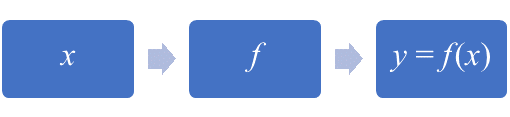
\includegraphics[width=1.0\textwidth]{function.png}
	\hspace{1mm}
	\caption{Function $f(x)$} 
	\label{fig:x}
\end{figure}

\section{Function p(x)}
The input dhātus are categorized as seṭ and aniṭ to determine whether an \texthindi{इ} is added before the addition of a pratyaya or not. This however, is different from the \texthindi{इ} that is added due to the addition of the \texthindi{णिच्} pratyaya. When the \texthindi{णिच्} pratyaya is added only \texthindi{इ} remains and the rest is removed. To differentiate between the two \texthindi{इ}s, only \texthindi{इ} is added when the addition is due to the input dhātu being seṭ, and when it is added due to the addition of the \texthindi{णिच्} pratyaya, it is written as \texthindi{इ(णिच्)} which should be read as \texthindi{इ} due to \texthindi{णिच्}. Note that this differentiation is required only when both types of \texthindi{इ} occur simulataneously in the same equation.  Thus \texthindi{इ(णिच्)} becomes a part of the prakṛti, whereas the \texthindi{इ} due to \texthindi{णिच्} pratyaya is a pratyaya. \\
The dhātus which have two or more vowels are called seṭ (with iṭ), and when a suffix is added to them an \texthindi{इ} comes. For dhātus which have one vowel, we need to see the instructions given in the Dhātupātha. They can either be seṭ or aniṭ depending upon the given instructions given. As it is a global function which is used in the definition of other pratyaya functions, it is important to define it here.\\
Define a function p(x) by, \\
\begin{equation}
	p(x)= \begin{cases}
		\text{\texthindi{इ}} & \text{if $x$ is \texthindi{ सेट्}}\\
		\phi&  \text{ if $x$ is \texthindi{ अनिट्}}\\
	\end{cases}
\end{equation}
\section{The $+$ operator}

\label{sec:operator}
The $+$ operator can be compared to Sandhi in grammar. It has been used extensively in the formulas. Some of the cases which might be observed in the various examples have been enumerated below.\\
For seṭ Dhātus:\\

\begin{center}
	\begin{tabular}{ p{4cm} p{4cm} p{4cm} }
		
		\texthindi{क्+इ=कि}&
		\texthindi{ख्+इ=खि}&
		\texthindi{ग्+इ=गि}\\
		\texthindi{घ्+इ=घि}&
		\texthindi{च्+इ=चि}&
		\texthindi{छ्+इ=छि}\\
		\texthindi{ज्+इ=जि}&
		\texthindi{ट्+इ=टि}&
		\texthindi{ठ्+इ=ठि}\\
		\texthindi{त्+इ=ति}&
		\texthindi{थ्+इ=थि}&
		\texthindi{द्+इ=दि}\\
		\texthindi{ध्+इ=धि}&
		\texthindi{प्+इ=पि}&
		\texthindi{ऊ+इ=वि}\\
		\texthindi{ए+इ=अयि}&
		\texthindi{ब्+इ=बि}&
		\texthindi{व्+इ=वि}\\
		\texthindi{भ+इ=भि}&
		\texthindi{फ्+इ=फि}&
		\texthindi{ण्+इ=णि}\\
		\texthindi{न्+इ=नि}&
		\texthindi{म्+इ=मि}&
		\texthindi{य्+इ=यि}\\
		\texthindi{ल्+इ=लि}&
		\texthindi{र्+इ=रि}&
		\texthindi{क्ष्+इ=क्षि}\\
		\texthindi{ष्+इ=षि}&
		\texthindi{स्+इ=सि}&
		\texthindi{ह्+इ=हि}\\
		\texthindi{श्+इ=शि}&
		\texthindi{झ्+इ=झि}&
		\texthindi{ञ्+इ=ञि}\\
		\texthindi{ङ्+इ=ङि}&
		\texthindi{ढ+इ=ढि}&
		\texthindi{ओ+इ=अवि}\\
		
	\end{tabular}
\end{center}


Similarly, for aniṭ dhātus:
\\
\begin{center}
	\begin{tabular}{ p{4cm} p{4cm} p{4cm}}
		\texthindi{क्+त=क्त}&
		\texthindi{ र्+त=र्त}&
		\texthindi{ द्+त=त्त}\\
		\texthindi{ ष्+त=ष्ट}&
		\texthindi{ च्+त=च्त}&
		\texthindi{ छ्+त=ष्ट}\\
		\texthindi{ ज्+त=क्त}&
		\texthindi{ ण्+त=न्त}&
		\texthindi{ त्+त=त्त}\\
		\texthindi{ ध्+त=ध्द}&
		\texthindi{ न्+त=न्त}&
		\texthindi{ प्+त=प्त}\\
		\texthindi{ भ्+त=ब्ध}&
		\texthindi{ म्+त=तं}&
		\texthindi{ श्+त=श्त}\\
		\texthindi{ स्+त=स्त}&
		\texthindi{ ह्+त= ण्ढ}&
		
	\end{tabular}
\end{center}

\section{Input Dhātus (x)}
The primary list of input dhātus are taken from Madhaviya Dhātuvṛtti which are enumerated in set $A$. Let $A$ be a set of all the dhātus after the Anubandha has been removed.\\

$A$ = [\texthindi{दा धा मा गा हा पा शा षा छा वा रा जा सा का या भा ला दरिद्रा स्था ज्या व्या क्षा ग्ला म्ला द्या श्रा द्रा ध्मा प्या श्या प्रा त्रा स्त्या घ्रा ध्रा म्ना ध्या स्ना प्सा ज्ञा ख्या ह्वा श्रि श्वि ज्रि स्मि जि कि हि रि पि धि इ सि शि चि मि चिरि जिरि प्री व्री ह्री भ्री क्षी व्ली प्ली क्री श्री री पी शी नी दी मी धी ली डी भी वी ई मी दीधी वेवी ऊर्णु कु ध्रु गु स्तु द्रु स्रु श्रु धु दु सु धु धू नु यु रु क्षु क्ष्णु स्नु उ गु कु घु ङु च्यु ज्यु प्रु प्लु रु ह्नु हु कु सु दु द्यु सु स्कु यु ब्रु नू धू मू सू पू दू लू नू क्नू धू सू भू स्वृ ध्वृ ह्वृ स्मृ स्पृ स्तृ हृ गृ घृ पृ दृ सृ ॠ जागृ धृ पृ दृ मृ धृ हृ भृ कृ वॄ भॄ मॄ पॄ स्तॄ कॄ शॄ दॄ तॄ जॄ झॄ गॄ नॄ ऋ(प्लुत) अक् शक् तक् चक् स्तक् कक् कख् बख् मख् नख् रख् लख् अग् लग् रग् सग् हग् ह्वग् ह्लग् स्तग् कग् घघ् सघ् दघ् वच् व्यच् खच् खम् पच् त्वच् सच् शच् मच् श्वच् कच् अज् यज् भज् त्यज् लज् जज् ध्रज् घ्वज् खज् गज् वज् व्रज् अट् घट् कट् वट् भट् णट् नट् पट् रट् लट् शट् सट् वट् जट् झट् भट् तट् खट् हट् पठ् मठ् रठ् शठ् वठ् कठ् हठ् अड् लड् कड् गड् अण् क्षण् फण् रण् मण् वण् भण् कण् क्वण् व्रण् भ्रण् ध्वण् श्रण् चण् शण् चण् रण् पण् अत् यत् चत् फत् क्वथ् पथ् मथ् व्यथ् प्रथ् श्रथ् श्लथ् क्लथ् क्रथ् अद् सद् शद् मद् बद् रद् नद् खद् वद् हद् पद् दद् स्वद् व्रद् श्खद् चद् बध् व्यध् रध् दध् वन् मन् तन् वन् जन् खन् सन् कन् स्वन् स्तन् ध्वन् धन् ध्रण् पन् हन् अन् स्वप् तप् वप् शप् क्रप् जप् चप् सप् रप् लप् त्रप् रफ् कब् रभ् लभ् जभ् यभ् नभ् गम् नम् यम् रम् भ्रम् शम् तम् दम् श्रम् शम् क्लम् क्षम् कम् क्रम् छम् झम् जम् जिम् चम् सम् स्तम् स्यम् वम् द्रम् अम् अय् दय् वय् पय् मय् चय् तय् नय् रय् वय् हय् त्वर् ज्वर् चर् त्सर् क्मर् क्षर् अल् फल् चल् जल् नल् पल् बल् सल् दल् शल् तल् ट्वल् स्थल् हल् ज्वल् ह्वल् ह्मल् स्खल् खल् गल् श्वल् मल् शल् वल् भल् कल् अव् मव् शव् अश् नश् मश् शश् वश् स्पश् चष् लष् छष् झष् मष् शष् जष् कष् खष् वष् भष् अस् उध्रस् ध्रस् घस् जस् तस् दस् मस् यस् वस् शस् सस् रस् लस् त्रस् स्नस् क्नस् ह्रस् व्लस् कस् घस् हस् प्रस् नस् ग्रस् ग्लस् वस् भ्यस् दह् वह् सह् नह् रह् मह् चह् ग्लह् ग्रह् अह् \\
	टिक् तिक् इख् लिख् तिग् स्तिघ् सिच् रिच् विच् निज् विज् तिज् इट् किट् खिट् शिट् सिट् चिट् बिट् विट् पिट् पिठ् क्षिण् कित् चित् श्वित् विथ् स्विद् मिद् क्षिद् मिद् स्विद् क्लिद् विद् भिद् क्षिद् विद् खिद् निद् मिद् सिध् विध् क्षिप् लिप् तिप् स्तिप् डिप् रिफ् तिम् स्तिम् इल् मिल् तिल् किल् चिल् विल् बिल् निल् हिल् मिल् शिल् सिल् ष्ठिव् क्षिव् सिव् दिव् स्रिव् दिश् लिश् रिश् विश् क्लिश् लिश् मिश् निश् पिश् इष् शिष् रिष् जिष् मिष् श्रिष् विष् ध्रिष् श्लिष् द्विष् विष् रिष् शिष् पिष् विष् त्विष् पिस् बिस् स्निह् दिह् लिह् मिह् प्लिह् \\
	कुक् उख् मुच् शुच् रुच् स्तुच् म्रुच् म्लुच् ग्रच् ग्लुच् शुच् कुच् उच् रुज् भुज् कुज् खुज् तुज् मुज् गुज् युज् भुज् स्फुट् रुट् लुट् घुट् कुट् पुट् मुट् त्रुट् तुट् चुट् छुट् घुट्  लुठ् रुठ् शुठ् उठ् मुड् प्रुड्हड् तुड् जुड् कुड् पुड् तुड् थुड् स्थुड् गुड् स्फुड् चुड् व्रुड् रुड् घुण् तुण् द्रुण् पुण् मुण् कुण् च्युत् श्चुत् श्च्युत् युत् जुत् द्युत् कुथ् पुथ् मुद् गुद् तुद् नुद् शुद् रुद् नुद् बुध् गुध् क्रुध् क्षुध् शुध् रुध् युध् अनुरुध् शुन् गुप् लुप् छुप् तुप् त्रुप् चुप् कुप् युप् रुप् लुप् तुफ् त्रुफ् गुफ् शुभ् स्तुभ् तुभ् क्षुभ् लुभ् क्षुभ् उभ् गुर् छुर् स्फुर् तुर् सुर् खुर् कुर् मुर् शुर् घुर् पुर् श्फुल् पुल् कुल् हुल् क्रुश् रुश् उष् शुष् तुष् दुष् पुष् व्युष् प्लुष् घुष् पुष् रुष् प्रुष् प्लुष् व्युष् मुष् कुष् जुष् बुस् मुस् कुस् तुस् श्नुस् दुह् तुह् सुह् रुह् ध्रुह् मुह् स्नुह् गुह् उह् \\
	वृक् ॠच् पृच् ॠज् धृज् गृज् वृज् मृज् सृज् भृज् कृड् भृड् मृड् पृड् ऋण् पृण् वृण् मृण् तृण् घृण् वृत् नृत् कृत् चृत् वृत् शृद् तृद् मृद् ऋध् गृध् वृध् शृध् मृध् कल्प् सृप् त्रृप् दृप् ऋफ् सृभ् दृभ् स्पृश् वृश् दृश् भृश् कृश् हृश् तृष् पृष् वृष् मृष् घृष हृष् धृष् कृष् ऋष् दृह् बृह् तृह् वृह् स्तृह् गृह् \\
	अन्क् तन्क् स्रन्क् शन्क् श्लन्क् शन्क् वन्क् मन्क् कन्क् श्वन्क् त्रन्क् शीक् टीक् तीक् द्रेक् ध्रेक् रेक् सेक् स्त्रेक् लोक् श्लोक् ढौक् त्रौक् ष्वष्क् वस्क् मस्क् फक्क् बुक्क् पुक्क् हिक्क् ओख् इन्ख् ईन्ख् उन्ख् वन्ख् मन्ख् रन्ख् नन्ख् लन्ख् राख् लाख् द्राख् ध्राख् शाख् श्लाख् अन्ग् इङ्ग रन्ग् लन्ग् वन्ग् मन्ग् तन्ग् शन्ग् श्लन्ग् रिन्ग् लिन्ग् थन्ग् युन्ग् जुन्ग् बुन्ग् वल्ग् अन्घ् मन्घ् रन्घ् लन्घ् वन्घ् मन्घ् शिन्घ् राघ् लाघ् द्राघ् श्लाघ् अञ्च् अर्च् लुञ्च् वञ्च् कुञ्च् चञ्च् तञ्च् त्वञ्च् म्रुञ्च् म्लुञ्च् ग्लुञ्च् तञ्च् कुञ्च् श्वन्च् शन्च् कन्च् कान्च् मुन्च् मन्च् पन्च् याच् लोच् वर्च् चर्च् व्रश्च् ऋच्छ आन्छ उन्छ् उञ्छ् उच्छ् प्रच्छ् लान्छ् वान्छ् हुर्च्छ् स्फूर्च्छ् मूर्च्छ् विच्छ् मिच्छ् युच्छ् लच्छ् ह्रीच्छ् म्लेच्छ् ऋन्ज् ईज् एज् उब्ज् अर्ज् अञ्ज् रञ्ज् भञ्ज् सञ्ज् गुन्ज् ध्रन्ज् धृन्ज् ध्वन्ज् खन्ज् लन्ज् लान्ज् जन्ज् तुन्ज् गन्ज् गृन्ज् मुन्ज् लाज् क्षीज् कूज् तेज् सर्ज् गर्ज् तर्ज् कर्ज् खर्ज् जर्ज् स्फूर्ज् मज्ज् क्षन्ज् निंज् शिंज् पिंज् स्वञ्ज् लज्ज् भ्रेज् भ्राज् राज् सज्ज् भ्रज्ज् झर्झ् उज्झ् अट्ट् घट्ट् वेष्ट् चेष्ट् गोष्ट् लोष्ट् रेट् रुन्ट् लुन्ट् म्लेट् शौट् यौट् एठ् अन्ठ् वन्ठ् मन्ठ् कन्ठ् मुन्ठ हेठ् कुन्ठ् लुन्ठ् शुन्ठ् रुन्ठ् कुन्ड् चुन्ड् गन्ड् मन्ड् वन्ड् भन्ड् चन्ड् शन्ड् तन्ड् पन्ड् कन्ड् खन्ड् हिन्ड् पिन्ड् हुन्ड् कुन्ड् मुन्ड् तुन्ड् बाड् द्राड् ध्राड् शाड् हेड् होड् क्रीड् व्रीड् हूड् म्रेड् हेड् होड् रोड् लोड् रौड् चुड्ड् कड्ड् अड्ड् ईड् ओण् पैण् शोण् श्रोण् श्लोण् घूर्ण् वेण् घिन्ण् घुन्ण् घृन्ण् धूर्ण् अन्त् संस्त् कुन्थ् पुन्थ् लुन्थ् मन्थ् ग्रन्थ् कुन्थ् श्रन्थ् ग्रन्थ् कत्थ् वेथ् नाथ् प्रोथ् अर्द् अन्द् इन्द् उन्द् उर्द् बुन्द् मेद् नेद् वन्द् भन्द् मन्द् स्पन्द् कन्द् क्रन्द् क्लन्द् श्विन्द् स्कुन्द् क्लिन्द् कूर्द् खूर्द् गूर्द् पर्द् स्वर्द् स्वाद् ह्राद् ह्लाद् सूद् स्यन्द् स्कन्द् नर्द् गर्द् तर्द् कर्द् खर्द् त्रन्द् कन्द् क्रन्द् क्लन्द् चन्द् नन्द् बिन्द् निन्द् क्लिन्द् खाद् इन्ध् एध् शुन्ध् बन्ध् राघ् साध् मेध् नाध् बाध् गाध् स्पर्ध् मान् दान् शान् धूप् तुम्प् त्रुम्प् पर्प् जल्प् पुष्प् कन्प् दीप् तेप् स्तेप् ग्लेप् वेप् केप् गेप् ग्लेप् मेप् रेप् लेप् आप् ॠम्फ् रन्फ् तुम्फ् त्रुम्फ् तृम्फ् दृम्फ् तुम्फ् गुम्फ् अर्ब् अन्ब् क्लीब् क्षीब् रन्ब् लन्ब् कुन्ब् लुन्ब् तुन्ब् चुन्ब् पर्ब् लर्ब् बर्ब् भर्ब् कर्ब् खर्ब् गर्ब् शर्ब् सर्ब् चर्ब् उम्भ् दम्भ् शुम्भ् सृम्भ् श्रम्भ् स्रम्भ् स्तन्भ् स्कन्भ् जृन्भ् शीभ् चीभ् रेभ् शल्भ् वल्भ् गल्भ् भाम् हम्म् स्तीम् मीम् ऊय् ईर्क्ष्य् ईर्ष्य् मव्य् शुच्य् हर्य् सूर्क्ष्य् चाय् ताय् क्ष्माय् स्फाय् पूय् क्नूय् प्याय् ईर् अभ्र् वभ्र् मभ्र् खोर् धोर् पूर् तूर् धूर् गूर् घूर् जूर् शूर् चूर् वेल् चेल् केल् खेल् क्ष्वेल् पेल् फेल् शेल् खोल् मील् श्मील् स्मील् क्ष्मील् पील् नील् शील् कील् कूल् शूल् तूल् पूल् मूल् खल्ल् चिल्ल् चुल्ल् फुल्ल् वेल्ल् वल्ल् कल्ल् मल्ल् भल्ल् इन्व् ऊर्व् अर्व् रन्व् धन्व् पिन्व् मिन्व् निन्व् हिन्व् दिन्व् धिन्व् जिन्व् रिन्व् कृण्व् पीव् मीव् तीव् नीव् जीव् क्षेव् मूर्व् तूर्व् थूर्व् दूर्व् धूर्व् गूर्व् पर्व् सर्व् मर्व् चर्व् भर्व् कर्व् खर्व् गर्व् शर्व् पूर्व् चीव् धाव् तेव् देव् सेव् गेव् ग्लेव् पेव् मेव् म्लेव् रेव् ईश् क्लेश् काश् वाश् भ्राश् भ्लाश् दंश् भ्रंश् दाश् ईष् ऊष् ईष् एष् चूष् तूष् पूष् मूष् लूष् रूष् शूष् यूष् जूष् भूष् घुन्ष् वर्ष् भाष् गेष् ग्लेष् पेष् जेष् नेष् प्रेष् रेष् हेष् ह्रेष् भेष् भ्रेष् भ्लेष् ईक्ष् उक्ष् अक्ष् तक्ष् रक्ष् त्रक्ष् स्त्रक्ष् नक्ष् वक्ष् जक्ष् निक्ष् मृक्ष् सूर्क्ष् कान्क्ष् वान्क्ष् मान्क्ष् द्रान्क्ष् ध्रान्क्ष् ध्वान्क्ष् भ्रक्ष् भ्लक्ष् त्वक्ष् दक्ष् ध्रिक्ष् शिक्ष् भिक्ष् दीक्ष् धुक्ष् वृक्ष् चक्ष् आस् स्रंस् ध्वंस् भ्रंस् आशन्स् कंस् निंस् कास् भास् नास् रास् आशास् दास् पेस् शास् चकास् हिंस् शंस् ईह् ऊह् अन्ह् अर्ह् तृंह् रन्ह् दृन्ह् बृन्ह् बन्ह् मन्ह् गर्ह् बर्ह् वर्ह् बल्ह् गल्ह् वल्ह् बाह् द्राह् वेह् जेह् गाह् माह् \\
	चुरादिगण- चि जि ज्रि प्री ली मी भू धू वृ पॄ जॄ वच् पट् घट् नट् तड् पत् तड् पत् श्रथ् नद् छद् वद् आसद् स्वद् तन् तप् दल् नल् जस् उध्रस् ग्रस् सह् रिच् दिव् शिष् रुज् युज् पुट् लुट् रुट् पुथ् गुप् कुप् जुष् पुष् घुष् पृच् वृज् मृज् वृत् छृद् शृध् वृध् तृप् दृभ् मृष् धृष् वल्क विष्क लोक् तर्क् शीक् चीक् टन्क् दुःख मार्ग् लिन्ग् लन्घ् रन्घ् लन्घ् लोच् पन्च् वन्च् अञ्च् अर्च् विच्छ् मिन्ज् पिन्ज् लुन्ज् भन्ज् तुन्ज् छन्ज् लन्ज् अन्ज् वन्ट् घन्ट् पुन्ट् चुन्ट् शुन्ठ् कन्ठ् दण्ड स्फुन्ड् लन्ड् खन्ड् कन्ड् कुन्ड् गुन्ड् खुन्ड् मन्ड् भन्ड् पन्ड् पिन्ड् लन्ड् वर्ण पर्ण चिन्त् पन्थ् ग्रन्थ् श्रन्थ् तुत्थ मिन्द् छन्द् अर्द् शुन्ध् मान् आप् धूप् चम्प् क्षम्प् चुम्ब् कुम्ब् लुम्ब् तुम्ब् जम्भ् कत्र चित्र मूत्र ईर् पूर् चीव् गर्व छिद्र मिश्र दंश् कुंश् भृंश् रुंश् रूक्ष त्रंस् पिंस् कुंस् दंस् रुंस् जंस् तंस् पंस् हिंस् दंस् अंह् बृंह् रंह् मंह् अर्ह् गर्ह् बर्ह् बल्ह् ज्ञा च्यु भू यु गृ घृ रक् लग् रच लज व्रज् गज् भज् नट् चट् घट् पट वट शठ श्वठ शठ् श्वठ् शठ् तड् खड् लड् श्रण् कण् gaṇa व्रण यत् श्रय् प्रथ् श्रथ कथ गद छद पद मद् बध् ध्वन स्तन ज्ञप् ह्लप् डप् अम् शम् स्यम् यम् व्यय वर स्वर चर् क्षल् तल् जल् कल् कल बल् चल् लल् गल् भल् पश् स्पश् लस् त्रस् नस् रस वस रह् मह रह चह तिज् स्मिट् चित् विद् डिप् क्षिप विल् बिल् तिल् इल् श्लिष् पिस् स्नेह् सुख मुच् चुट् मुट् स्फुट् त्रुट् पुट् शुठ् जुड् कुण गुण चुद् मुद् स्तुप् चुर् तुल् दुल् पुल् चुल् रुष् कुह मृग पृथ् कल्प् कृप वृष् गृह स्पृह बुक्क् नक्क् धक्क् चक्क् चुक्क् श्वल्क् वल्क् शुल्क् अर्क् विष्क् निष्क् अङ्क अङ्ग धेक सूच चर्च् मर्च् म्लेच्छ् पिच्छ् पूज् मार्ज् अर्ज् तर्ज् ऊर्ज् भाज सभाज कीट् घट्ट् खट्ट् सट्ट् स्फिट्ट् कुट्ट् पुट्ट् चुट्ट् अट्ट् सुट्ट् कूट् कूट खेट क्षोट लुण्ठ् ईड् पीड् चूर्ण् वर्ण् कूण् तूण् भ्रूण् क्रूण मुस्त् पुस्त् बुस्त् श्वर्त् कॄत् बस्त् वात संकेत केत अर्थ गूर्द् शब्द् सूद् आक्रन्द् छर्द् छेद अन्ध्र गन्ध् वर्ध् मान् ऊन स्तेन रूप शूर्प् सम्ब् शम्ब् शुल्ब् लाभ भाम साम ग्राम सङ्ग्राम गोम स्तोम कुस्म् सार पार तीर सूत्र कुमार श्वभ्र् गूर् शूर वीर सत्र यन्त्र् तन्त्र् मन्त्र् कुन्द्र् पूल् मूल् पाल् स्थूल शील वेल पल्यूल सान्त्व् भूष् लूष् गवेष लक्ष् पक्ष् यक्ष् भक्ष् म्रक्ष् पुंस् धूस् ब्रूस् भर्त्स् कुत्स् वास निवास अंस बर्ह् अर्ह् सुख दुःख लिट लाट गद्गद अगद वेद मगध इषुध कुषुभ तरण चरण वरण चुरण तुरण भुरण सपर अरर अम्बर संवर लेखा रेखा लेला मेधा एला केला खेला इला मही हृणी मन्तु वल्गु कण्डू असू असु इर् इरज् भिषज् भिष्णज् लेट् लोट् इरस् उषस् तन्तस् पम्पस् द्रवस् तिरस् उरस् पयस् संभूयस्}]
\\
These primary dhātus are 1943 in total. However, the input dhātus are not limited to these dhātus in set $A$. We can also derive a new dhātu by adding a san pratyaya to the dhātus of set $A$. By ‘3.1.32 \texthindi{सनाद्यन्ताः धातवः}’ the derived dhātus also becomes a dhātu as it says that whenever we add a \texthindi{सनादि} pratyaya to a Dhātu, it again becomes a Dhātu. \\

There are several ways of deriving Dhātus:\\
By adding a suffix to any Dhātu (enlisted in set $B$)\\
Derving Dhātus from nouns i.e. nāmdhātu $(j(x)) $(enlisted in set $C$)\\

List of \texthindi{सनादि} pratyayas in Aṣhṭādhyāyī with their respective sūtra numbers:\\
\begin{itemize}
	\item \texthindi{3.1.5 सन्}
	\item \texthindi{3.1.8 क्यच्}
	\item \texthindi{3.1.9 काम्यच्}
	\item \texthindi{3.1.11 क्यङ्}
	\item \texthindi{3.1.13 क्यष्}
	\item \texthindi{3.1.20 णिङ्}
	\item \texthindi{3.1.21 णिच्}
	\item \texthindi{3.1.22 यङ्}
	\item \texthindi{3.1.27 यक्}
	\item \texthindi{3.1.28 आय्}
	\item \texthindi{3.1.29 ईयङ्}
\end{itemize}
$B$ is a set of all the derived dhātus that are derived by adding san pratyayas to the set $A$. \\
$C$ is a set of nāmdhātus\\
\begin{equation}
	x \epsilon (A \cup B \cup C)
\end{equation}


%%\chapter{णिच् function}

\section{\texthindi{णिच्} function}
णिच् pratyaya is used in the sense of ‘inspiration’ for 1st to 10th gaṇa. It is easier to understand the syntax of a causative sentence in relation to a non-causative or a pre-causative sentence. Generally, in a causative construction, there are two agents, a) the agent of original action, and b) the agent of causation or instigation. If the original verb is transitive, then there may be an object of the original verb.\\
The णिच् pratyaya is enlisted among the sanādi pratyayas. The causative of a tenth gaṇa verb may be identical with the original in form, though different in meaning. One can have, in theory, numerous degrees of causativeness, and yet the outward form reains the same:\\
\texthindi{गच्छति }    “X goes.”\\
\texthindi{गमयति }  “Y makes X go.”\\ 
\texthindi{गमयति} “Z makes Y make X go.”\\ 
\texthindi{गमयति} “A makes Z make Y make X go.”\\ 
------
------
The difference between different degrees of causativeness is apparent from the form itself, but must be understood from the syntax of the rest of the sentence (Madhav M. Deshpande, 2007, pp. 341-342). Now this \texthindi{णिच्} pratyaya can be added to a derived dhātu \texthindi{णिच्}(x) again.\\

In this Chapter, the results obtained from all the algorithms are presented in separate sub-sections along with the detailed investigations using topographic and observatory measurements. Multi-temporal analyses of the results are also presented. 

\subsection{Definition of \texthindi{णिच्} function}
\texthindi{णिच्}: set of dhātus → set of derived dhātus/ prātipadikas of \texthindi{णिच्}

\subsection{Cases for \texthindi{णिच्} function}

\textbf{Case I:}\\
$x(1)=c$, $x(2)=c$/\texthindi{आ/ई/ऊ/ए}\\
\begin{equation}
	{\texthindi{णिच्}}(x) = x + \text{\texthindi{ इ}} 
\end{equation}


\begin{table}[h!]
	\begin{center}
		\begin{tabular}{ |c|c|c|c| } 
			\hline
			$x$ & $x(1)$ & $x(2)$ & \texthindi{णिच्($x$)}\\
			\hline
			\texthindi{स्पर्ध्}&$c$&$c$&\texthindi{स्पर्धि}\\
			\texthindi{नाथ्}&$c$&\texthindi{आ}&\texthindi{नाथि}\\
			\texthindi{ शीक् }&$c$&\texthindi{ ई }&\texthindi{ शीकि }\\
			\texthindi{ तूष् }&$c$&\texthindi{ ऊ}&\texthindi{ तूषि }\\
			\texthindi{ एध् }&$c$&\texthindi{ ए }&\texthindi{ एधि }\\
			\hline
		\end{tabular}
		\caption{Examples of \texthindi{णिच्} function Case I}
		\label{table:6.1}
		
	\end{center}
\end{table}

\textbf{Case II:}\\
$x(1)=c$, $x(2)=\text{\texthindi{अ}}$
\begin{equation}
	\text{\texthindi{णिच्}}(x) = x[\text{\texthindi{अ }}\xrightarrow{2} \text{\texthindi{आ}}]+ \text{\texthindi{इ}}  
\end{equation}


\begin{table}[h!]
	\begin{center}
		\begin{tabular}{ |c|c|c|c| } 
			\hline
			$x$ & $x(1)$ & $x(2)$ & \texthindi{णिच्($x$)}\\
			\hline
			\texthindi{ दद् }&$c$&$c$&\texthindi{ दादि }\\
			\texthindi{दध्}&$c$&\texthindi{अ}&\texthindi{दाधि}\\
			\hline
		\end{tabular}
		\caption{Examples of \texthindi{णिच्} function Case II}
		\label{table:6.2}
	\end{center}
\end{table}


\textbf{Case III:}\\
$x(1)=c$, $x(2)=$\texthindi{इ/उ/ऋ }
\begin{equation}
	\text{\texthindi{णिच्}}(x) = x[\text{\texthindi{ इ उ ऋ }}\xrightarrow{2} \text{\texthindi{ ए ओ अर् }}]+ \text{\texthindi{इ}}  
\end{equation}

\begin{table}[h!]
	\begin{center}
		
		\begin{tabular}{ |c|c|c|c| } 
			\hline
			$x$ & $x(1)$ & $x(2)$ & \texthindi{णिच्($x$)}\\
			\hline
			\texthindi{ पिट् }&$c$&\texthindi{ इ }&\texthindi{ पेटि }\\
			\texthindi{ मुद् }&$c$&\texthindi{ उ }&\texthindi{ मोदि }\\
			\texthindi{ भृज् }&$c$&\texthindi{ ऋ }&\texthindi{ भर्जि }\\
			\hline
		\end{tabular}
		\caption{Examples of \texthindi{णिच्} function Case III}
		\label{table:6.3}
	\end{center}
	
\end{table}

\textbf{Case IV:}\\
$x(1) =$ \texthindi{इ/ई उ/ऊ ऋ}
\begin{equation}
	\text{\texthindi{णिच्}}(x) = x[\text{\texthindi{ इ/ई उ/ऊ ऋ }}\xrightarrow{1} \text{\texthindi{ आय् आव् आर् }}]+ \text{\texthindi{इ}}
\end{equation}


\begin{table}[h!]
	\begin{center}
		\begin{tabular}{ |c|c|c| } 
			\hline
			$x$ & $x(1)$ & \texthindi{णिच्($x$)}\\
			\hline
			\texthindi{ क्षि }&\texthindi{ इ }&\texthindi{ क्षायि }\\
			\texthindi{ नी }&\texthindi{ ई }&\texthindi{ नायि }\\
			\texthindi{ घु }&\texthindi{ उ }&\texthindi{ घावि }\\
			\texthindi{ सू }&\texthindi{ ऊ }&\texthindi{ सावि }\\
			\texthindi{ वृ }&\texthindi{ ऋ }&\texthindi{ सावि }\\
			\hline
		\end{tabular}
		\caption{Examples of \texthindi{णिच्} function Case IV}
		\label{table:6.4}
	\end{center}
\end{table}


\textbf{Case V:}\\
$x(1) =$ \texthindi{आ}
\begin{equation}
	\text{\texthindi{णिच्}}(x) = x + \text{\texthindi{ प् }} +  \text{\texthindi{इ}}
\end{equation}

\begin{table}[h!]
	\begin{center}
		
		\begin{tabular}{ |c|c|c| } 
			\hline
			$x$ & $x(1)$ & \texthindi{णिच्($x$)}\\
			\hline
			\texthindi{ का }&\texthindi{ आ }&\texthindi{ कापि }\\
			\hline
		\end{tabular}
		\caption{Examples of \texthindi{णिच्} function Case V}
		\label{table:6.5}
	\end{center}
	
\end{table}

\textbf{Case VI:}\\ 
This case only appears in \texthindi{चुरादिर्गण} that is the 10th gaṇa\\
$x(1)=$\texthindi{अ}\\
\begin{equation}
	\text{\texthindi{णिच्}}(x) = x[\text{\texthindi{अ}}\xrightarrow{1}\phi]+ \text{\texthindi{इ}}
\end{equation}

\begin{table}[h!]
	\begin{center}
		
		\begin{tabular}{ |c|c|c| } 
			\hline
			$x$ & $x(1)$ & \texthindi{णिच्($x$)}\\
			\hline
			\texthindi{ रच }&\texthindi{ अ }&\texthindi{ रचि }\\
			\hline
		\end{tabular}
		\caption{Examples of \texthindi{णिच्} function Case VI}
		\label{table:6.6}
	\end{center}
	
\end{table}

\textbf{Case VII:}\\
If $x є$ [\texthindi{क्रम् तम् रम् शम् श्रम् जन् वध्}]
\begin{equation}
	\text{\texthindi{णिच्}}(x) = x + \text{\texthindi{इ}}  
\end{equation}

\begin{table}[h!]
	\begin{center}
		
		\begin{tabular}{ |c|c| } 
			\hline
			$x$ & \texthindi{णिच्($x$)}\\
			\hline
			\texthindi{ क्रम् }&\texthindi{ क्रमि }\\
			\texthindi{ तम् }&\texthindi{ तमि }\\
			\texthindi{ रम् }&\texthindi{ रमि }\\
			\texthindi{ शम् }&\texthindi{ शमि }\\
			\texthindi{ श्रम् }&\texthindi{ श्रमि }\\
			\texthindi{ जन् }&\texthindi{ जनि }\\
			\texthindi{ वध् }&\texthindi{ वधि }\\
			\hline
		\end{tabular}
		\caption{Examples of \texthindi{णिच्} function Case VII}
		\label{table:6.7}
	\end{center}
	
\end{table}

\textbf{Case VIII:}\\
If $x$ $\epsilon$ [\texthindi{ऋ ह्री व्ली री क्नूयी क्ष्मायी}]\\
\begin{equation}
	\text{\texthindi{णिच्}}(x) =c(1^{\prime}) + c(2^{\prime})* +v[\text{\texthindi{ ऋ ई उ/ऊ }}\xrightarrow{1^{\prime}} अ\text{\texthindi{ र् ए ओ}}] + \text{\texthindi{ प् }}+ \text{\texthindi{इ}}
\end{equation}
\\
$c(2^{\prime})$ will be added only when $x(2^{\prime})$ is not a vowel.
\begin{table}[h!]
	\begin{center}
		\begin{tabular}{ |c|c|c| } 
			\hline
			$x$ & $c(1^{\prime}) + c(2^{\prime})* + v[\text{\texthindi{ऋ ई ऊ}} \xrightarrow{1^{\prime}} \text{\texthindi{अर् ए ओ}}]$ & \texthindi{णिच्($x$)}\\
			\hline
			\texthindi{ ऋ }&\texthindi{ अर् }&\texthindi{ अर्पि }\\
			\texthindi{ ह्री }&\texthindi{ ह्रे }&\texthindi{ ह्रेपि }\\
			\texthindi{ व्ली }&\texthindi{ व्ले }&\texthindi{ व्लेपि }\\
			\texthindi{ री }&\texthindi{ रे }&\texthindi{ रेपि }\\
			\texthindi{ क्नूयी }&\texthindi{ क्नो }&\texthindi{ क्नोपि }\\
			\texthindi{ क्ष्मायी }&\texthindi{ क्ष्मा }&\texthindi{ क्ष्मापि }\\
			\texthindi{ रुह्}&\texthindi{ रो }&\texthindi{ रोपि }\\
			\hline
		\end{tabular}
		\caption{Examples of \texthindi{णिच्} function Case VI}
		\label{table:6.8}
	\end{center}
	
\end{table}

\textbf{Case IX:}
\\If $x$ $\epsilon $ [\text{\texthindi{शो छो षो ह्वेञ् व्येञ् वेञ् पा}}]\\
\begin{equation}
	\text{\texthindi{णिच्}}(x) =c(1^{\prime}) + c(2’)* +v[\text{\texthindi{ ओ ए }}\xrightarrow{1’} अ\text{\texthindi{ आ }}] + \text{\texthindi{ य् }}+ \text{\texthindi{इ}}
\end{equation}
$c(2’)$ will be added only when $x(2’)$ is not a vowel.\\


\begin{table}[h!]
	\begin{center}
		\begin{tabular}{ |c|c|c| } 
			\hline
			$x$ & $c(1^{\prime}) + c(2’)* + v[\text{\texthindi{ओ ए}} \xrightarrow{1’} \text{\texthindi{आ }}]$ & \texthindi{णिच्($x$)}\\
			\hline
			\texthindi{ शो}&	\texthindi{ शा}&	\texthindi{ शायि}\\
			\texthindi{ छो}&	\texthindi{ छा}&	\texthindi{ छायि}\\
			\texthindi{ षो}&	\texthindi{ सा}&	\texthindi{ सायि}\\
			\texthindi{ ह्वेञ्}&	\texthindi{ ह्वा}&	\texthindi{ ह्वायि}\\
			\texthindi{ व्येञ्}&	\texthindi{ व्या}&	\texthindi{ व्यायि}\\
			\texthindi{ वेञ्}&	\texthindi{ वा}&	\texthindi{ वायि}\\
			\texthindi{ पा}&	\texthindi{ पा}&	\texthindi{ पायि}\\
			\hline
		\end{tabular}
		\caption{Examples of \texthindi{णिच्} function Case IX}
		\label{table:6.9}
	\end{center}
\end{table}




\textbf{Case X:}\\
If $x$ $\epsilon$ [\texthindi{स्फायी}]\\
\begin{equation}
	\text{\texthindi{णिच्}}(x) = c(1^{\prime}) + c(2^{\prime}) +v(1^{\prime})+ \text{\texthindi{ व् }}+ \text{\texthindi{इ}}
\end{equation}
\begin{table}[h!]
	\begin{center}
		\begin{tabular}{ |c|c|c| } 
			\hline
			$x$&	$c(1^{\prime}) + c(2^{\prime}) + v(1^{\prime})$&	\texthindi{णिच्($x$)}\\
			\hline
			\texthindi{ स्फायी}&	\texthindi{ स्फा}&	\texthindi{ स्फावि}\\
			\hline
		\end{tabular}
		\caption{Examples of \texthindi{णिच्} function Case X}
		\label{table:6.10}
	\end{center}
	
\end{table}

\textbf{Case XI:}\\
If $x$ $\epsilon$ [\texthindi{शदॢ}]\\
\begin{equation}
	\text{\texthindi{णिच्}}(x) = c(1^{\prime}) +v(1^{\prime})+ \text{\texthindi{ व् }}+ \text{\texthindi{इ}}
\end{equation}
\begin{table}[h!]
	\begin{center}
		\begin{tabular}{ |c|c|c| } 
			\hline
			$x$&	$c(1^{\prime}) +  v(1^{\prime})$&	\texthindi{णिच्($x$)}\\
			\hline
			\texthindi{ शदॢी}&	\texthindi{ शाा}&	\texthindi{ शाति}\\
			\hline
		\end{tabular}
		\caption{Examples of \texthindi{णिच्} function Case XI}
		\label{table:6.11}
	\end{center}
	
\end{table}


Thus, we looked at the cases of the णिच् function which gives the output in the form of a णिजन्त word. Now let us look into a kṛt pratyaya, i.e. a Tumun Pratyaya.
%\section{Tumun Function}
\subsection{Definition}
\subsection{Cases for {\texthindi{तुमुन्}} function}
Type 1: x does not belong to the 10th gaṇa.\\
\textbf{Case I:}\\
If x $\not\in$  {{ \texthindi{दीधी वेवी दी (दीण् दिवादिर्गण) चिरि जिरि}}}\\ 
x(1) = \texthindi{इ/ई उ/ऊ ऋ/ॠ}, x(2) = c,\\ 
then,\\
\begin{equation}
	\text{\texthindi{ तुमुन् }}(x) = x[\text{\texthindi{इ/ई उ/ऊ ऋ/ॠ }}\xrightarrow{1} \text{\texthindi{ ए ओ अर् }}] + p(x) +  \text{\texthindi{ तुम् }}  
\end{equation} 

\begin{table}[h!]
	\begin{center}
		\begin{tabular}{ |c|c|c| } 
			\hline
			x&	  x[\texthindi{इ/ई उ/ऊ ऋ/ॠ } $\xrightarrow{1} $ \texthindi{ ए ओ अर् }] + p(x) &	\text{\texthindi{ तुमुन्}}(x) \\
			\hline
			\texthindi{ श्रि}&	\texthindi{ श्रयि}&	\texthindi{ श्रयितुम्}\\
			\hline
		\end{tabular}
		\caption{Examples of \texthindi{तुमुन्} function Case I}
		\label{table:6.12}
	\end{center}
\end{table}

Here we have used the ‘+’ rule \texthindi{ए}+\texthindi{इ}=\texthindi{अयि}
\\
\textbf{Case II:}\\
If x $\epsilon$ [\texthindi{दीधी वेवी चिरि जिरि}] 
then\\
\begin{equation}
	\text{\texthindi{तुमुन्}}(x) = x[\text{\texthindi{इ/ई}}  \xrightarrow{1} \phi] + p(x) + \text{\texthindi{तुम्}}\\
\end{equation}

\begin{table}[h!]
	\begin{center}
		\begin{tabular}{ |c|c|c| } 
			\hline
			x&	F(x) = x[\text{\texthindi{इ/ई}}  $\xrightarrow{1} \phi$] + p(x)&	\texthindi{तुमुन्}(x) \\
			\hline
			\texthindi{दीधी}&	\texthindi{दीधि}&	\texthindi{दीधितुम्}\\
			\texthindi{वेवी}&	\texthindi{वेवि}&	\texthindi{वेवितुम्}\\
			\hline
		\end{tabular}
		\caption{Examples of \texthindi{तुमुन्} function Case II}
		\label{table:6.13}
	\end{center}
\end{table}


\textbf{Case III:}\\ 
If x = \texthindi{दी} and belongs to 4th gaṇa (\texthindi{दिवादिर्गण})\\
then\\
\begin{equation}
	\text{\texthindi{तुमुन्}}(x) = x[\text{\texthindi{ई}}  \xrightarrow{1} \text{\texthindi{आ}}] + p(x) + \text{\texthindi{तुम्}}
\end{equation}

\begin{table}[h!]
	\begin{center}
		\begin{tabular}{ |c|c|c| } 
			\hline
			x&	x[\text{\texthindi{ई}} $ \xrightarrow{1}$ \text{\texthindi{ आ}}] + p(x)&	\texthindi{तुमुन्} (x)  \\
			\hline
			\texthindi{ दी }&	\texthindi{ दा }&	\texthindi{ दातुम् }\\
			\hline
		\end{tabular}
		\caption{Examples of \texthindi{तुमुन्} function Case III}
		\label{table:6.14}
	\end{center}
\end{table}

\textbf{Case IV:}\\
If x $\not\in$ {\texthindi{कुट् पुट् गुज् गुढ् ढिप् चुर् स्फुट् मुट् त्रुट् तुट् चुट् लुट् कृढ् कुढ् पुढ् घुट् तुढ् थुढ् स्फुढ् स्फुर् स्फुल् स्फुढ् स्फुर् स्फुल् कुढ् बुढ् क्रुढ् भुढ् गुर् व्रीढ् दृश् सृज् तिज् गुप् विज् तिज्} (1 gaṇa \texthindi{भ्वादिर्गण}) \texthindi{गुप्} (10 gaṇa) \texthindi{गुप्} (1 gaṇa \texthindi{भ्वादिर्गण गुपू रक्षणे}) \texthindi{गुप्} (1 gaṇa \texthindi{भ्वादिर्गण गोप गोपने}) \texthindi{लिह् मिह्}}\\
x(1) = c, x(2) = \texthindi{इ उ ऋ},\\ 
then\\

\begin{equation}
	\text{\texthindi{ तुमुन् }}(x) = x[\text{\texthindi{ \texthindi{इ} उ ऋ }}\xrightarrow{2} \text{\texthindi{ ए ओ अर् }}]+ p(x) + \text{\texthindi{ तुम् }}  
\end{equation}


\begin{table}[h!]
	\begin{center}
		\begin{tabular}{ |c|c|c| } 
			\hline
			x&	 x[\text{\texthindi{ \texthindi{इ} उ ऋ }}$\xrightarrow{2}$ \text{\texthindi{ ए ओ अर् }}]+ p(x)&	\texthindi{तुमुन्}(x) \\
			\hline
			\texthindi{ विथ्}&	\texthindi{ वेथि}&	\texthindi{ वेथितुम्}\\
			\texthindi{ मुद्}&	\texthindi{ मोदि}&	\texthindi{ मोदितुम्}\\
			\texthindi{ वृत्}&	\texthindi{ वर्ति}&	\texthindi{ वर्तितुम्} \\ 
			\hline
		\end{tabular}
		\caption{Examples of \texthindi{तुमुन्} function Case IV}
		\label{table:6.15}
	\end{center}
\end{table}

\textbf{Case V:}\\
If x $\epsilon$ [\texthindi{कुट् पुट् गुज् गुढ् ढिप् चुर् स्फुट् मुट् त्रुट् तुट् चुट् लुट् कृढ् कुढ् पुढ् घुट् तुढ् थुढ् स्फुढ् स्फुर् स्फुल् स्फुढ् स्फुर् स्फुल् कुढ् बुढ् क्रुढ् भुढ् गुर भृढ् गुर् व्रीढ् कु गु ध्रु}]\\
or if x(1)= \texthindi{अ/आ}/c; x(2)= c/v $\neq$ \texthindi{इ/उ/ऋ}; \\
then\\
\begin{equation}
	\text{\texthindi{ तुमुन् }}(x) = x+ p(x) + \text{\texthindi{ तुम् }}  
\end{equation}

\begin{table}[h!]
	\begin{center}
		\begin{tabular}{ |c|c|c| } 
			\hline
			x&	x+ p(x)&	\texthindi{तुमुन्}(x) \\
			\hline
			\texthindi{ कुट्}&	\texthindi{कुटि}&	\texthindi{ कुटितुम्}\\
			\hline
		\end{tabular}
		\caption{Examples of \texthindi{तुमुन्} function Case V}
		\label{table:6.16}
	\end{center}
\end{table}

\textbf{Case VI:}\\
If x $\epsilon$ {\texthindi{लिह् मिह्}}\\
then \\
\begin{equation}
	\text{\texthindi{ तुमुन् }}(x) = x[\text{\texthindi{ इ }}\xrightarrow{2} \text{\texthindi{ ए }}; [\text{\texthindi{ ह् }}\xrightarrow{1} \text{\texthindi{ ढ् }}]+ \text{\texthindi{ उम् }}  
\end{equation}


\begin{table}[h!]
	\begin{center}
		\begin{tabular}{ |c|c|c| } 
			\hline
			x&	 x[\text{\texthindi{ इ }} $\xrightarrow{2}$ \text{\texthindi{ ए }}; \text{\texthindi{ ह् }} $\xrightarrow{1}$ \text{\texthindi{ ढ् }}]&	\texthindi{तुमुन्}(x) \\
			\hline 
			\texthindi{लिह्}&	\texthindi{लेढ्}&	\texthindi{लेढुम्} \\ 
			\hline
		\end{tabular}
		\caption{Examples of \texthindi{तुमुन्} function Case VI}
		\label{table:6.17}
	\end{center}
\end{table}

\textbf{Case VII:}\\
If x $\epsilon$ [\texthindi{दृश् सृज्}]\\
then\\ 
\begin{equation}
	\text{\texthindi{ तुमुन् }}(x) = x[\text{\texthindi{ ऋ }}\xrightarrow{2} \text{\texthindi{ र् }}]+ \text{\texthindi{ तुम् }}  
\end{equation}

\begin{table}[h!]
	\begin{center}
		\begin{tabular}{ |c|c|c| } 
			\hline
			x&	x[\text{\texthindi{ ऋ }}$\xrightarrow{2}$ \text{\texthindi{ र् }}]  &	\texthindi{ तुमुन्}(x)  \\
			\hline
			\texthindi{ दृश्}&	\texthindi{ द्रश्}&	\texthindi{ द्रष्टुम्}\\
			\texthindi{ सृज्}&	\texthindi{ स्रज्}&	\texthindi{ स्रष्टुम्} \\ 
			\hline
		\end{tabular}
		\caption{Examples of \texthindi{तुमुन्} function Case VII}
		\label{table:6.18}
	\end{center}
\end{table}

\textbf{Case VIII:}\\
If x $\not\in$ [\texthindi{रुह् वह् बध् दरिद्रा}]\\
x(1) $\neq$ \texthindi{इ/ई उ/ऊ ऋ/ॠ};  x(2) $\neq$ \texthindi{इ उ ऋ},\\
then\\ 
\begin{equation}
	\text{\texthindi{ तुमुन् }}(x) = x + p(x) + \text{\texthindi{ तुम्} }
\end{equation}

\begin{table}[h!]
	\begin{center}
		\begin{tabular}{ |c|c|c| } 
			\hline
			x&	x+p(x)&	\texthindi{ तुमुन्(x) }\\
			\hline
			\texthindi{ तन्क् }&	\texthindi{ तन्कि }&	\texthindi{ तन्कितुम् } \\ 
			\hline
		\end{tabular}
		\caption{Examples of \texthindi{तुमुन्} function Case VIII}
		\label{table:6.19}
	\end{center}
\end{table}

\textbf{Case IX:}\\
If x $\epsilon$ [\texthindi{रुह् वह्}]\\
then\\
\begin{equation}
	\text{\texthindi{ तुमुन् }}(x) = x[\text{\texthindi{ उ अ }}\xrightarrow{2} \text{\texthindi{ ओ }}]+p(x)+ \text{\texthindi{ ह् }}\xrightarrow{1} \phi + \text{\texthindi{ तुम् }}  
\end{equation}

\begin{table}[h!]
	\begin{center}
		\begin{tabular}{ |c|c|c| } 
			\hline
			x&	x[\texthindi{ उ अ } $\xrightarrow{2}$ \texthindi{ ओ }]+p(x)+ \texthindi{ ह् }$\xrightarrow{1}$ $\phi$&	\texthindi{ तुमुन्}(x) \\
			\hline
			\texthindi{ रुह् }&	\texthindi{रो}&	\texthindi{ रोढुम्}\\
			\texthindi{ वह् }&	\texthindi{वो }&	\texthindi{ वोढुम् }\\
			\hline
		\end{tabular}
		\caption{Examples of \texthindi{तुमुन्} function Case IX}
		\label{table:6.20}
	\end{center}
\end{table}

\textbf{Case X:}\\
If x = \texthindi{दरिद्रा}\\
then\\
\begin{equation}
	\text{\texthindi{ तुमुन् }}(x) = x[\text{\texthindi{ आ }}\xrightarrow{1} \phi]+p(x)+  \text{\texthindi{ तुम् }}  
\end{equation} 

\begin{table}[h!]
	\begin{center}
		\begin{tabular}{ |c|c|c| } 
			\hline
			x&	x[\text{\texthindi{आ}}  $\xrightarrow{1}$ $\phi$] + p(x)&	\texthindi{तुमुन्}(x)\\
			\hline
			\texthindi{ दरिद्रा }&	\texthindi{ दरिद्रि }&	\texthindi{ दरिद्रितुम् }\\
			\hline
		\end{tabular}
		\caption{Examples of \texthindi{तुमुन्} function Case X}
		\label{table:6.21}
	\end{center}
\end{table}

\textbf{Case XI:}\\
x(2)= \texthindi{र् व्}, x(3)= \texthindi{उ}\\
then\\
\begin{equation}
	\text{\texthindi{ तुमुन् }}(x) = x[\text{\texthindi{ उ }}\xrightarrow{3} \text{\texthindi{ ऊ }}]+p(x)+  \text{\texthindi{ तुम् }}  
\end{equation}

\begin{table}[h!]
	\begin{center}
		\begin{tabular}{ |c|c|c| } 
			\hline
			x &	x[\text{\texthindi{ उ }}$\xrightarrow{3}$ \text{\texthindi{ ऊ }}]+p(x)&	\texthindi{तुमुन्}(x)\\
			\hline
			\texthindi{उर्द}&	\texthindi{ऊर्दि}&	\texthindi{ऊर्दितुम्}\\
			\texthindi{उर्व}&	\texthindi{ऊर्वि}&	\texthindi{ऊर्वितुम्} \\ 
			\hline
		\end{tabular}
		\caption{Examples of \texthindi{तुमुन्} function Case XI}
		\label{table:6.22}
	\end{center}
\end{table}




\textbf{Type 2: x belongs to the 10th gaṇa.}\\
\texthindi{तुम्} = \texthindi{तुम्(णिच्}(x))\\
y = \texthindi{णिच्}(x)\\
y(1) = \texthindi{इ}\\
\begin{equation}
	\text{\texthindi{ तुमुन्(णिच् }}(x)) = \text{\texthindi{ तुम्}} y  
\end{equation}
then\\
\begin{equation}
	\text{\texthindi{ तुमुन्}}(y) = y[\texthindi{इ}\xrightarrow{1}\texthindi{ए}] + p(x) + \text{\texthindi{ तुम्}}  
\end{equation}
Note: - The output of function \texthindi{णिच्}(x) is treated as input for \texthindi{तुमुन्}(x) and the same Cases as Type 1 can be used.\\
Examples:\\

\begin{table}[h!]
	\begin{center}
		\begin{tabular}{ |c|c|c|c|c|}
			\hline
			Case &	x&	y = \texthindi{णिच्}(x)&	y[\texthindi{इ}  $\xrightarrow{1}$ \texthindi{ए}] + p(x) &	\texthindi{तुम्(णिच्}(x))\\
			\hline
			I &	\texthindi{स्पर्ध्}&	\texthindi{स्पर्धि}&	\texthindi{स्पर्धयि}&	\texthindi{स्पर्धयितुम्}\\
			I &	\texthindi{दध्}&	\texthindi{दधि}&	\texthindi{दधयि}&	\texthindi{दधयितुम्}\\
			I &	\texthindi{नाथ्}&	\texthindi{नाथि}&	\texthindi{नाथयि}&	\texthindi{नाथयितुम्}\\
			II &	\texthindi{दद्}&	\texthindi{दादि}&	\texthindi{दादयि}&	\texthindi{दादयितुम्}\\
			III &	\texthindi{पिट्}&	\texthindi{पेटि}&	\texthindi{पेटयि}&	\texthindi{पेटयितुम्}\\
			III &	\texthindi{मुद्}&	\texthindi{मोदि}&	\texthindi{मोदयि}&	\texthindi{मोदयितुम्}\\
			IV &	\texthindi{नी}&	\texthindi{नायि}&	\texthindi{नाययि}&	\texthindi{नाययितुम्}\\
			\hline
		\end{tabular}
		\caption{Examples of \texthindi{तुमुन्} function if x belongs to the 10th gaṇa}
		\label{table:6.23}
	\end{center}
\end{table}

\textbf{Multivalued functions:}\\ 
In some Cases, there are multiple words from a single dhātu. To account for such Cases, the concept of multivaled functions is used where a single input to the \texthindi{तुमुन्} (x) function generates multiple outputs.\\
\textbf{Case I:}\\
If x $\epsilon$ \texthindi{सिध्(षिधू)} 
then\\
\begin{equation}
	\text{\texthindi{तुमुन् }} (x) = 
	\begin{cases}
		x [\text{\texthindi{ इ/ई उ/ऊ ऋ/ॠ }}\xrightarrow{2}\text{\texthindi{ ए ओ अर् }}]+ \text{\texthindi{इ}} + \text{\texthindi{तुम्}}\\
		x [\text{\texthindi{ इ/ई उ/ऊ ऋ/ॠ }}\xrightarrow{2} \text{\texthindi{ ए ओ अर् }}]+ \phi + \text{\texthindi{तुम्}}\\
	\end{cases}
\end{equation}

\begin{table}[h!]
	\begin{center}
		\begin{tabular}{ |c|c|c| } 
			\hline
			x &
			$
				\begin{cases}
							x [\text{\texthindi{ इ/ई उ/ऊ ऋ/ॠ }}\xrightarrow{2}\text{\texthindi{ ए ओ अर् }}]+ \text{\texthindi{इ}} + \text{\texthindi{तुम्}}\\
							x [\text{\texthindi{ इ/ई उ/ऊ ऋ/ॠ }}\xrightarrow{2} \text{\texthindi{ ए ओ अर् }}]+ \phi + \text{\texthindi{तुम्}}\\
				\end{cases}
			$ &
			\texthindi{तुमुन्}(x)\\
			\hline
			\multirow{2}{*}{\texthindi{सिध्}}&	
			\text{\texthindi{सेधि }}&
			\text{\texthindi{सेधितुम्}}\\ 
			&
			\text{\texthindi{सेध्}}&
			\text{\texthindi{सेद्धुम्}}\\
			\hline
		\end{tabular}
		\caption{Examples of Case I for multivalued functions of \texthindi{तुमुन्} }
		\label{table:6.24}
	\end{center}
\end{table}

\textbf{Case II:}\\
If x $\epsilon$ [\texthindi{स्वृ सू (षूङ् अदादिर्गणः) धू}]\\
then\\
\begin{equation}
	\text{\texthindi{तुमुन्}} (x) = 
	\begin{cases}
		x[\text{\texthindi{ इ/ई उ/ऊ ऋ/ॠ }}\xrightarrow{1}\text{\texthindi{ ए ओ अर् }}]+ \text{\texthindi{इ}} + \text{\texthindi{तुम्}}\\
		x[\text{\texthindi{ इ/ई उ/ऊ ऋ/ॠ }}\xrightarrow{1} \text{\texthindi{ ए ओ अर् }}]+ \phi + \text{\texthindi{तुम्}}\\
	\end{cases}
\end{equation}

\begin{table}[h!]
	\begin{center}
		\begin{tabular}{ |c|c|c| } 
			\hline
			x & 
			$
				\begin{cases}
					x [\text{\texthindi{ इ/ई उ/ऊ ऋ/ॠ }} \xrightarrow{1} \text{\texthindi{ ए ओ अर् }}]+ \text{\texthindi{इ}} \\
					x [\text{\texthindi{ इ/ई उ/ऊ ऋ/ॠ }} \xrightarrow{1} \text{\texthindi{ ए ओ अर् }}]+ \phi \\
				\end{cases}
			$
			& \texthindi{तुमुन्}(x)\\
			\hline
			\multirow{2}{*}{\texthindi {सू }}&	
			\texthindi{ सवि}&
			\texthindi{सवितुम्}\\ 
			& \texthindi{सो}&
			\texthindi{सोतुम्}\\
			\hline
			\multirow{2}{*}{\texthindi { स्वृ }}&
			\texthindi{ स्वरि }&
			\texthindi {स्वरितुम् }\\ 
			&
			\texthindi{ स्वर् }&
			\texthindi {स्वर्तुम् }\\
			\hline
			
		\end{tabular}
		\caption{Examples of Case II for multivalued functions of \texthindi{तुमुन्} }
		\label{table:6.25}
	\end{center}
\end{table}

\textbf{Case III:}\\
If x $\epsilon$ \texthindi{पॄ(3 जुहोत्यादिर्गणः) जॄ झॄ वृ कॄ गॄ स्तॄ कॄ वॄ शॄ पॄ भॄ मॄ दृ जॄ नृ कृ ऋ ॠ (तुदादिगण) गृ})\\ 
then\\

\begin{equation}
	\text{\texthindi{तुमुन्}} (x) = 
	\begin{cases}
		x [\text{\texthindi{ इ/ई उ/ऊ ऋ/ॠ }} \xrightarrow{1} \text{\texthindi{ ए ओ अर् }} ]+  \text{\texthindi{इ}}  +  \texthindi{तुम्}\\
		x [\texthindi{ इ/ई उ/ऊ ऋ/ॠ } \xrightarrow{1} \texthindi{ ए ओ अर् } ]+  \texthindi{ई}  +  \texthindi{तुम्}\\
	\end{cases}
\end{equation}

\begin{table}[h!]
	\begin{center}
		\begin{tabular}{ |c|c|c| } 
			\hline
			x & 
			$ \begin{cases}
				x [\text{\texthindi{ इ/ई उ/ऊ ऋ/ॠ }}\xrightarrow{1} \text{\texthindi{ ए ओ अर् }}+ \text{\texthindi{इ}}\\
				x [\text{\texthindi{ इ/ई उ/ऊ ऋ/ॠ}}\xrightarrow{1} \text{\texthindi{ ए ओ अर् }}]+ \text{\texthindi{ई}}\\
			\end{cases} $
			& \texthindi{तुमुन्}(x)\\
			\hline
			\multirow{2}{*}{\texthindi{वृ}}
			&\texthindi{वरि}
			&\texthindi{वरितुम्}\\ 
			&\texthindi{वरी}
			&\texthindi{वरीतुम्}\\
			\hline
			\multirow{2}{*}{\texthindi{कॄ}}
			&\texthindi{करि }
			&\texthindi{करितुम् }\\
			&\texthindi{करी}
			&\texthindi{करीतुम्}\\
			\hline
		\end{tabular}
		\caption{Examples of Case III for multivalued functions of \texthindi{तुमुन्} }
		\label{table:6.26}
	\end{center}
\end{table}\

\textbf{Case IV:}\\
If x $\epsilon$ [\texthindi{सृप् कृष्}]\\
then\\

\begin{equation}
	\text{\texthindi{तुमुन्}} (x) = 
	\begin{cases}
		x[\text{\texthindi{ ऋ/ॠ }}\xrightarrow{2}\text{\texthindi{ अर् }}] + \text{\texthindi{इ}} + \text{\texthindi{तुम्}}\\
		x[\text{\texthindi{ ऋ/ॠ }}\xrightarrow{2}\text{\texthindi{ र् }}] + \phi + \text{\texthindi{तुम्}}\\
	\end{cases}
\end{equation}

\begin{table}[h!]
	\begin{center}
		\begin{tabular}{ |c|c|c| } 
			\hline
			x &
			$ \begin{cases}
				x[\text{\texthindi{ ऋ/ॠ }}\xrightarrow{2}\text{\texthindi{ अर् }}] + \text{\texthindi{इ्}}\\
				x[\text{\texthindi{ ऋ/ॠ }}\xrightarrow{2}\text{\texthindi{ र् }}] + \phi \\
			\end{cases} $
			& \texthindi{तुमुन्}(x)\\
			\hline
			\multirow{2}{*}{\texthindi{सृप्}}
			&\texthindi{सर्पि}
			&\texthindi{सर्पितुम् }\\
			&\texthindi{स्रप्}
			&\texthindi{स्रप्तुम्}\\
			\multirow{2}{*}{\texthindi{कृष्}}
			&\texthindi{कर्षि }
			&\texthindi{कर्षितुम् }\\
			&\texthindi{क्रष्}
			&\texthindi{क्रष्टुम्}\\
			\hline
		\end{tabular}
		\caption{Examples of Case IV for multivalued functions of \texthindi{तुमुन्} }
		\label{table:6.27}
	\end{center}
\end{table}

\textbf{Case V:}\\
If x =\texthindi{ऊर्णु}\\
then\\

\begin{equation}
	\texthindi{तुमुन्} (x)  = 	
	\begin{cases}
		x[\text{\texthindi{उ}}\xrightarrow{1}\text{\texthindi{ओ}}\xrightarrow{1}\text{\texthindi{अव्}}] + \text{\texthindi{इ}} + \text{\texthindi{तुम्}}\\
		x[\text{\texthindi{उ}}\xrightarrow{1}\text{\texthindi{ अव्}}] + \text{\texthindi{इ}}+ \text{\texthindi{तुम्}}\\
	\end{cases}
\end{equation}

\begin{table}[h!]
	\begin{center}
		\begin{tabular}{ |c|c|c| } 
			\hline
			x & 
			$ \begin{cases}
				x[\text{\texthindi{उ}}\xrightarrow{1}\text{\texthindi{ओ}}\xrightarrow{1}\text{\texthindi{अव्}}] + \text{\texthindi{इ}}\\
				x[\text{\texthindi{उ}}\xrightarrow{1}\text{\texthindi{ अव्}}] + \text{\texthindi{इ}}\\
			\end{cases} $ & \texthindi{तुमुन्}(x)\\
			\hline
			\multirow{2}{*}{\texthindi{ऊर्णु}}
			&\texthindi{ऊर्णवि}
			&\texthindi{ऊर्णवितुम् }\\
			&\texthindi{ऊर्णुवि}
			&\texthindi{ऊर्णुवितुम्}\\

		\hline
		\end{tabular}
		\caption{Examples of Case V for multivalued functions of \texthindi{तुमुन्} }
		\label{table:6.28}
	\end{center}
\end{table}

\textbf{Case VI:}\\
If x $\epsilon$ \texthindi{ली}\\
then\\

\begin{equation}
	\texthindi{तुमुन्} (x)  = 
	\begin{cases}
		x[\text{\texthindi{ई}}\xrightarrow{1}\text{\texthindi{ए}}]+ \text{\texthindi{तुम्}}\\
		x[\text{\texthindi{ई}}\xrightarrow{1}\text{\texthindi{आ}}]+ \text{\texthindi{तुम्}}\\
	\end{cases}
\end{equation}

\begin{table}[h!]
	\begin{center}
		\begin{tabular}{ |c|c|c| } 
			\hline
			x & $\begin{cases}
				x[\text{\texthindi{ई}}\xrightarrow{1}\text{\texthindi{ए}}]\\
				x[\text{\texthindi{ई}}\xrightarrow{1}\text{\texthindi{आ}}]\\
			\end{cases}$ & \texthindi{तुमुन्}(x)\\
			\hline
			\multirow{2}{*}{\texthindi{ली}}
			&\texthindi{ले}
			&\texthindi{लेतुम्}\\ 
			&\texthindi{ला}
			&\texthindi{लातुम्}\\
			\hline
		\end{tabular}
		\caption{Examples of Case VI for multivalued functions of \texthindi{तुमुन्} }
		\label{table:6.29}
	\end{center}
\end{table}

\textbf{Case VII:}\\
If x $\epsilon$ \texthindi{गुप्} (1 gaṇa \texthindi{भ्वादिर्गणः (गुपू रक्षणे)}\\
then\\
\begin{equation}
	\texthindi{तुमुन्} (x) = 	
	\begin{cases}
		x[\text{\texthindi{ इ/ई उ/ऊ ऋ/ॠ}}\xrightarrow{2}\text{\texthindi{ ए ओ अर्}}]+ \text{\texthindi{इ}} + \text{\texthindi{तुम्}}\\
		x[\text{\texthindi{ इ/ई उ/ऊ ऋ/ॠ}}\xrightarrow{2}\text{\texthindi{ ए ओ अर्}}]+ \phi + \text{\texthindi{तुम्}}\\
		x[\text{\texthindi{ इ/ई उ/ऊ ऋ/ॠ}}\xrightarrow{2}\text{\texthindi{ ए ओ अर्}}]+ \text{\texthindi{इ}} + \text{\texthindi{आय्}}+ \text{\texthindi{तुम्}}\\
	\end{cases}
\end{equation}

\begin{table}[h!]
	\begin{center}
		\begin{tabular}{ |c|c|c| } 
			\hline
			x & 
			$\begin{cases}
				x[\texthindi{ इ/ई उ/ऊ ऋ/ॠ}\xrightarrow{2}\texthindi{ ए ओ अर्}]+ \texthindi{इ}\\
				x[\texthindi{ इ/ई उ/ऊ ऋ/ॠ}\xrightarrow{2}\texthindi{ ए ओ अर्}]+ \phi \\
				x[\texthindi{ इ/ई उ/ऊ ऋ/ॠ}\xrightarrow{2}\texthindi{ ए ओ अर्}]+ \texthindi{इ} + \texthindi{आय्}\\
			\end{cases}$ 
			&\multirow{4}{*}{\texthindi{तुमुन्}(x)}\\
			\hline
			\multirow{3}{*}{\texthindi{गुप्}}
			&\texthindi{गोपि }
			&\texthindi{गोपितुम्}\\ 
			&\texthindi{गोप्}
			&\texthindi{गोप्तुम् }\\
			&\texthindi{गोपायि}
			&\texthindi{गोपायितुम्}\\
			\hline
		\end{tabular}
		\caption{Examples of Case VII for multivalued functions of \texthindi{तुमुन्} }
		\label{table:6.30}
	\end{center}
\end{table}

\textbf{Case VIII:}\\
If x $\epsilon$ \texthindi{गुप्} (1 gaṇa \texthindi{भ्वादिर्गणः गु॒प गोपने})\\

then\\
\begin{equation}
	\texthindi{तुमुन्}(x) = 	\begin{cases}
		x[\text{\texthindi{उ}}\xrightarrow{2}\text{\texthindi{ओ}}]+\text{\texthindi{अय्}}+ \text{\texthindi{इ}} + \text{\texthindi{तुम्}}\\
		\text{\texthindi{जु}} + x + \text{\texthindi{स्}} + \text{\texthindi{इ}} + \text{\texthindi{तुम्}}\\
	\end{cases}
\end{equation}


\begin{table}[h!]
	\begin{center}
		\begin{tabular}{ |c|c|c| } 
			\hline
			x &
			$\begin{cases}
				x[\text{\texthindi{उ}}\xrightarrow{2}\text{\texthindi{ओ}}]+\text{\texthindi{अय्}}\\
				\text{\texthindi{जु}} + x + \text{\texthindi{स्}}\\
			\end{cases}$ & \texthindi{तुमुन्}(x)\\
			\hline
			\multirow{2}{*}{\texthindi{गुप्}}
			&\texthindi{गोपय्}
			&\texthindi{गोपयितुम्}\\ 
			&\texthindi{जुगुप्स्}
			&\texthindi{जुगुप्सितुम्}\\
			\hline
		\end{tabular}
		\caption{Examples of Case VIII for multivalued functions of \texthindi{तुमुन्} }
		\label{table:6.31}
	\end{center}
\end{table}

\textbf{Case IX:}\\
If x $\epsilon$ [\texthindi{रुष् रिष् लुभ् क्लिद् लुभ् इष्}]\\
then\\
\begin{equation}
	\texthindi{तुमुन्}(x) = 	\begin{cases}
		x[\text{\texthindi{ इ\/ई उ\/ऊ ऋ\/ॠ}}\xrightarrow{2}\text{\texthindi{ ए ओ अर्}}]+ \text{\texthindi{इ}} + \text{\texthindi{तुम्}}\\
		x[\text{\texthindi{ इ\/ई उ\/ऊ ऋ\/ॠ}}\xrightarrow{2}\text{\texthindi{ ए ओ अर्}}]+ \phi + \text{\texthindi{तुम्}}\\
	\end{cases}
\end{equation}

\begin{table}[h!]
	\begin{center}
		\begin{tabular}{ |c|c|c| } 
			\hline
			x & 
			\texthindi{तुमुन्}(x) =
			$\begin{cases}
				x[\texthindi{ इ\/ई उ\/ऊ ऋ\/ॠ}\xrightarrow{2}\texthindi{ ए ओ अर्}]+ \texthindi{इ} \\
				x[\texthindi{ इ\/ई उ\/ऊ ऋ\/ॠ}\xrightarrow{2}\texthindi{ ए ओ अर्}]+ \phi \\
			\end{cases}$ & 
			\texthindi{तुमुन्}(x) \\ 
			\hline
			\multirow{2}{*}{\texthindi{रिष्}}
			&\texthindi{रेषि}
			&\texthindi{रेषितुम्}\\
			&\texthindi{रेष्}
			&\texthindi{रेष्टुम्}\\
			\multirow{2}{*}{\texthindi{लुभ्}}
			&\texthindi{लोभि}
			&\texthindi{लोभितुम्}\\
			&\texthindi{लोभ्}
			&\texthindi{लोब्धुम्}\\
			\hline
		\end{tabular}
		\caption{Examples of Case IX for multivalued functions of \texthindi{तुमुन्} }
		\label{table:6.32}
	\end{center}
\end{table}

\textbf{Case X:}\\
If x $\epsilon$ \texthindi{गुह्} (1 gaṇa \texthindi{भ्वादिर्गणः) गृह्} (1 gaṇa \texthindi{भ्वादिर्गणः)}\\
then\\
\begin{equation}
	\texthindi{तुमुन्}(x) = 	\begin{cases}
		x[\text{\texthindi{ उ ऋ}}\xrightarrow{2}\text{\texthindi{ ऊ अर्}}]+ \text{\texthindi{इ}} + \text{\texthindi{तुम्}}\\
		x[\text{\texthindi{ उ ऋ}}\xrightarrow{2}\text{\texthindi{ ओ अर्}}]]+ \text{\texthindi{ह्}}\rightarrow\phi + \text{\texthindi{ढुम्}}\\
	\end{cases}
\end{equation}

\begin{table}[h!]
	\begin{center}
		\begin{tabular}{ |c|c|c| } 
			\hline
			x & 
			\texthindi{तुमुन्}(x) = 	
			$\begin{cases}
				x[\text{\texthindi{ उ ऋ}}\xrightarrow{2}\text{\texthindi{ ऊ अर्}}]+ \text{\texthindi{इ}}\\
				x[\text{\texthindi{ उ ऋ}}\xrightarrow{2}\text{\texthindi{ ओ अर्}}]]+ \text{\texthindi{ह्}}\rightarrow\phi \\
			\end{cases}$ & 
			\texthindi{तुमुन्}(x) \\ 
			\hline
			\multirow{2}{*}{\texthindi{ गुह्}}
			&\texthindi{ गूहि}
			&\texthindi{ गूहितुम्}\\
			&\texthindi{ गो}
			&\texthindi{ गोढुम्}\\
			\multirow{2}{*}{\texthindi{ गृह्}}
			&\texthindi{ गर्हि}
			&\texthindi{ गर्हितुम्}\\ 
			&\texthindi{ गर्}
			&\texthindi{ गर्ढुम्}\\
			\hline
		\end{tabular}
		\caption{Examples of Case X for multivalued functions of \texthindi{तुमुन्} }
		\label{table:6.33}
	\end{center}
\end{table}


\textbf{Case XI:}\\
If x $\epsilon$ \texthindi{तिज्} (1 gaṇa \texthindi{भ्वादिर्गणः})
then\\
\begin{equation}
	\texthindi{तुमुन्}(x) = 	\begin{cases}
		x[\text{\texthindi{इ}}\xrightarrow{2}\text{\texthindi{ए}}]+\text{\texthindi{अय्}}+ \text{\texthindi{इ}} + \text{\texthindi{तुम्}}\\
		\text{\texthindi{ति}} + x[\text{\texthindi{ज्}}\xrightarrow{1}\text{\texthindi{क्ष्}}] +  \text{\texthindi{इ}} + \text{\texthindi{तुम्}}\\
	\end{cases}
\end{equation}


\begin{table}[h!]
	\begin{center}
		\begin{tabular}{ |c|c|c| } 
			\hline
			x & 
			\texthindi{तुमुन्}(x) = 	
			$\begin{cases}
				x[\text{\texthindi{इ}}\xrightarrow{2}\text{\texthindi{ए}}]+\text{\texthindi{अय्}}\\
				\text{\texthindi{ति}} + x[\text{\texthindi{ज्}}\xrightarrow{1}\text{\texthindi{क्ष्}}]\\
			\end{cases}$ & 
			\texthindi{तुमुन्}(x) \\ 
			\hline
			\multirow{2}{*}{\texthindi{तिज्}}
			&\texthindi{तेजय्}
			&\texthindi{तेजयितुम्}\\
			&\texthindi{तितिक्ष्}
			&\texthindi{तितिक्षितुम्}\\
			\hline
		\end{tabular}
		\caption{Examples of Case XI for multivalued functions of \texthindi{तुमुन्} }
		\label{table:6.34}
	\end{center}
\end{table}

\textbf{Case XII:}\\
If x $\epsilon$ \texthindi{कित्} (1 gaṇa \texthindi{भ्वादिर्गणः})\\
then\\
\begin{equation}
	\texthindi{तुमुन्}(x) = 	
	\begin{cases}
		x[\text{\texthindi{इ}}\xrightarrow{2}\text{\texthindi{ए}}]+\text{\texthindi{अय्}}+ \text{\texthindi{इ}} + \text{\texthindi{तुम्}}\\
		\text{\texthindi{चि}} + x + \text{\texthindi{स्}} +  \text{\texthindi{इ}} + \text{\texthindi{तुम्}}\\
	\end{cases}
\end{equation}

\begin{table}[h!]
	\begin{center}
		\begin{tabular}{ |c|c|c| } 
			\hline
			x & 
			\texthindi{तुमुन्}(x) = 	
			$\begin{cases}
				x[\text{\texthindi{इ}}\xrightarrow{2}\text{\texthindi{ए}}]+\text{\texthindi{अय्}}\\
				\text{\texthindi{चि}} + x + \text{\texthindi{स्}}\\
			\end{cases}$ & \texthindi{तुमुन्}(x) \\ 
			\hline
			\multirow{2}{*}{\texthindi{कित्}}
			&\texthindi{केतय्}
			&\texthindi{केतयितुम्}\\ 
			&\texthindi{चिकित्स्}
			&\texthindi{चिकित्सितुम्}\\
			\hline
		\end{tabular}
		\caption{Examples of Case XII for multivalued functions of \texthindi{तुमुन्} }
		\label{table:6.35}
	\end{center}
\end{table}

\textbf{Case XIII:}\\
If x $\epsilon$ \texthindi{तृप् दृप् (दृप हर्षमोहनयोः (दिवादिर्गणः))}\\
then\\

\begin{equation}
	\texthindi{तुमुन्}(x) = 
	\begin{cases}
		x[\text{\texthindi{ ॠ}}\xrightarrow{2}\text{\texthindi{ अर्}}]+ \phi + \text{\texthindi{तुम्}}\\
		x[\text{\texthindi{ ॠ}}\xrightarrow{2}\text{\texthindi{ र्}}]+ \phi + \text{\texthindi{तुम्}}\\
		x[\text{\texthindi{ ॠ}}\xrightarrow{2}\text{\texthindi{ अर्}}]+ \text{\texthindi{इ}} + \text{\texthindi{तुम्}}\\
	\end{cases}
\end{equation}


\begin{table}[h!]
	\begin{center}
		\begin{tabular}{ |c|c|c| } 
			\hline
			x & 
			\texthindi{तुमुन्}(x) = 	
			$\begin{cases}
				x[\text{\texthindi{ ॠ}}\xrightarrow{2}\text{\texthindi{ अर्}}]+ \phi\\
				x[\text{\texthindi{ ॠ}}\xrightarrow{2}\text{\texthindi{ र्}}]+ \phi\\
				x[\text{\texthindi{ ॠ}}\xrightarrow{2}\text{\texthindi{ अर्}}]+ \text{\texthindi{इ}}\\
			\end{cases}$ & \texthindi{तुमुन्}(x) \\ 
			\hline
			\multirow{3}{*}{\texthindi{दृप्}}
			&\texthindi{दर्प्}
			&\texthindi{दर्पतुम्}\\ 
			&\texthindi{द्रप्}
			&\texthindi{द्रप्तुम्}\\
			&\texthindi{दर्पि}
			&\texthindi{दर्पितुम्}\\
			\hline
		\end{tabular}
		\caption{Examples of Case XIII for multivalued functions of \texthindi{तुमुन्} }
		\label{table:6.36}
	\end{center}
\end{table}

\textbf{Case XIV:}\\
If x $\epsilon$ [\texthindi{द्रुह् मुह् स्नुह् स्निह्}]\\
then\\
\begin{equation}
	\texthindi{तुमुन्}(x) = 	
	\begin{cases}
		x[\texthindi{ इ उ}\xrightarrow{2}\texthindi{ ए ओ}]+ \phi + \texthindi{तुम्}\\
		x[\texthindi{ इ उ }\xrightarrow{2}\texthindi{ ए ओ }]+ \phi + \texthindi{तुम्}\\
		x[\texthindi{ इ उ}\xrightarrow{2}\texthindi{ ए ओ }]+ \texthindi{इ} + \texthindi{तुम्}\\
	\end{cases}
\end{equation}

\begin{table}[h!]
	\begin{center}
		\begin{tabular}{|c|c|} 
			\hline
			x & \texthindi{तुमुन्}(x)\\
			\hline
			\multirow{3}{*}{\texthindi{मुह्}}
			&\texthindi{मोग्धुम्}\\
			&\texthindi{मोढुम्}\\
			&\texthindi{मोहितुम्}\\
			\multirow{3}{*}{\texthindi{स्निह्}}
			&\texthindi{स्नेग्धुम् }\\
			&\texthindi{स्नेढुम् }\\
			&\texthindi{स्नेहितुम्}\\
			\hline
		\end{tabular}
		\caption{Examples of Case XIV for multivalued functions of \texthindi{तुमुन्} }
		\label{table:6.37}
	\end{center}
\end{table}

\textbf{Case XV:}\\
If x $\epsilon$ [\texthindi{कृष् स्पृश् मृश्}]\\
then\\

\begin{equation}
	\texthindi{तुमुन्}(x) = 	
	\begin{cases}
		x[\text{\texthindi{ॠ}}\xrightarrow{2}\text{\texthindi{अर्}}+ \phi + \text{\texthindi{टुम्}}\\
		x[\text{\texthindi{ॠ}}\xrightarrow{2}\text{\texthindi{र्}}+\phi + \text{\texthindi{टुम्}}\\
	\end{cases}
\end{equation}

\begin{table}[h!]
	\begin{center}
		\begin{tabular}{ |c|c|c| } 
			\hline
			x & 
			\texthindi{तुमुन्}(x) = 	
			$\begin{cases}
				x[\text{\texthindi{ॠ}}\xrightarrow{2}\text{\texthindi{अर्}}+ \phi\\
				x[\text{\texthindi{ॠ}}\xrightarrow{2}\text{\texthindi{र्}}+\phi\\
			\end{cases}$ & \texthindi{तुमुन्}(x) \\ 
			\hline
			\multirow{2}{*}{\texthindi{कृष्}}
			&\texthindi{कर्ष्}
			&\texthindi{कर्ष्टुम् }\\
			&\texthindi{क्रष्}
			&\texthindi{क्रष्टुम्}\\	
			\multirow{2}{*}{\texthindi{मृश्}}
			&\texthindi{मर्ष् }
			&\texthindi{मर्ष्टुम् }\\
			&\texthindi{म्रष्}
			&\texthindi{म्रष्टुम्}\\
			\hline
		\end{tabular}
		\caption{Examples of Case XV for multivalued functions of \texthindi{तुमुन्} }
		\label{table:6.38}
	\end{center}
\end{table}

\textbf{Case XVI:}\\
If x $\epsilon$ [\texthindi{वृह् तृह् स्तृह्}]\\
then\\ 
\begin{equation}
	\texthindi{तुमुन्}(x) = 	
	\begin{cases}
		x[\text{\texthindi{ॠ}}\xrightarrow{2}\text{\texthindi{अर्}}+ \text{\texthindi{इ}}+ + \text{\texthindi{तुम्}}\\
		x[\text{\texthindi{ॠ}}\xrightarrow{2}\text{\texthindi{र्}}+ \text{\texthindi{ह्}} \rightarrow \phi + \text{\texthindi{ढुम्}}\\
	\end{cases}
\end{equation}

\begin{table}[h!]
	\begin{center}
		\begin{tabular}{ |c|c|c| } 
			\hline
			x & 
			\texthindi{तुमुन्}(x) = 	
			$\begin{cases}
				x[\text{\texthindi{ॠ}}\xrightarrow{2}\text{\texthindi{अर्}}+ \phi\\
				x[\text{\texthindi{ॠ}}\xrightarrow{2}\text{\texthindi{र्}}+\phi\\
			\end{cases}$ & \texthindi{तुमुन्}(x)\\
			\hline
			\multirow{2}{*}{\texthindi{वृह्}}
			&\texthindi{वर्हि}
			&\texthindi{वर्हितुम्}\\
			&\texthindi{वर्}
			&\texthindi{वर्ढुम्}\\
			\multirow{2}{*}{\texthindi{तृह्}}
			&\texthindi{तर्हि}
			&\texthindi{तर्हितुम्}\\
			&\texthindi{तर्}
			&\texthindi{तर्ढुम्}\\
			\hline
		\end{tabular}
		\caption{Examples of Case XVI for multivalued functions of \texthindi{तुमुन्} }
		\label{table:6.39}
	\end{center}
\end{table}

\textbf{Case XVII:}\\
If x $\epsilon$ \texthindi{कुष्}\\
then\\

\begin{equation}
	\texthindi{तुमुन्}(x) = 	
	\begin{cases}
		x[\text{\texthindi{ उ}}\xrightarrow{2}\text{\texthindi{ ओ}}+ \text{\texthindi{इ}}+ \text{\texthindi{तुम्}}\\
		\text{\texthindi{निष्}} + x[\text{\texthindi{ उ}}\xrightarrow{2}\text{\texthindi{ ओ}}+ \phi + \text{\texthindi{तुम्}}\\
		\text{\texthindi{निष्}} + x[\text{\texthindi{ उ}}\xrightarrow{2}\text{\texthindi{ ओ}}+ \text{\texthindi{इ}}+ \text{\texthindi{तुम्}}\\
	\end{cases}
\end{equation}


\begin{table}[h!]
	\begin{center}
		\begin{tabular}{ |c|c|c| } 
			\hline
			x & 	
			$\begin{cases}
				x[\text{\texthindi{ उ}}\xrightarrow{2}\text{\texthindi{ ओ}}+ \text{\texthindi{इ}}\\
				\text{\texthindi{निष्}} + x[\text{\texthindi{ उ}}\xrightarrow{2}\text{\texthindi{ ओ}}+ \phi \\
				\text{\texthindi{निष्}} + x[\text{\texthindi{ उ}}\xrightarrow{2}\text{\texthindi{ ओ}}+ \text{\texthindi{इ}}\\
			\end{cases}$ 
			&\texthindi{तुमुन्}(x)\\
			\hline
			\multirow{3}{*}{\texthindi{कुष्}}
			&\texthindi{कोषि}
			&\texthindi{कोषितुम्}\\  
			&\texthindi{निष्कोष् }
			&\texthindi{निष्कोष्टुम् }\\
			&\texthindi{निष्कोषि}
			&\texthindi{निष्कोषितुम्}\\
			\hline
		\end{tabular}
		\caption{Examples of Case XVII for multivalued functions of \texthindi{तुमुन्} }
		\label{table:6.40}
	\end{center}
\end{table}


\begin{equation}
	\texthindi{तुमुन्}(x) = 	
	\begin{cases}
		x[\text{\texthindi{ ॠ}}\xrightarrow{2}\text{\texthindi{आर्}}+\text{\texthindi{इ}}+\text{\texthindi{तुम्}}\\
		x[\text{\texthindi{ ॠ}}\xrightarrow{2}\text{\texthindi{आर्}}+\phi+\text{\texthindi{तुम्}}\\
	\end{cases}
\end{equation}

\begin{table}[h!]
	\begin{center}
		\begin{tabular}{ |c|c|c| } 
			\hline
			x & 	
			$\begin{cases}
				x[\text{\texthindi{ ॠ}}\xrightarrow{2}\text{\texthindi{आर्}}+\text{\texthindi{इ}}\\
				x[\text{\texthindi{ ॠ}}\xrightarrow{2}\text{\texthindi{आर्}}+\phi\\
			\end{cases} $& \texthindi{तुमुन्}(x)  \\ 
			\hline
			\multirow{2}{*}{\texthindi{मृज्}}
			&\texthindi{मार्जयि}
			&\texthindi{मार्जयितुम्}\\
			&\texthindi{मार्जि}
			&\texthindi{मार्जितुम्}\\
			\hline
		\end{tabular}
		\caption{Examples of Case XVIII for multivalued functions of \texthindi{तुमुन्} }
		\label{table:6.41}
	\end{center}
\end{table}

\textbf{Case XIX:}\\
If x $\epsilon$ \texthindi{अज्}\\
then\\

\begin{equation}
	\texthindi{तुमुन्}(x) = 	
	\begin{cases}
		x+\text{\texthindi{इ}}+\text{\texthindi{तुम्}}\\
		\text{\texthindi{वे}}+\text{\texthindi{तुम्}}\\
	\end{cases}
\end{equation}


\begin{table}[h!]
	\begin{center}
		\begin{tabular}{|c|c|} 
			\hline
			x & \texthindi{तुमुन्}(x) \\ 
			\hline
			\multirow{2}{*}{\texthindi{अज्}}
			&\texthindi{अजितुम् }\\
			&\texthindi{वेतुम्}\\
			\hline
		\end{tabular}
		\caption{Examples of Case XIX for multivalued functions of \texthindi{तुमुन्} }
		\label{table:6.42}
	\end{center}
\end{table}

\textbf{Case XX:}\\
If x $\epsilon$ [\texthindi{त्रप् क्षम् कल्प् अश् अञ्ज् तन्च्}]\\
then\\
\begin{equation}
	\texthindi{तुमुन्}(x) = 	
	\begin{cases}
		x+\text{\texthindi{इ}}+\text{\texthindi{तुम्}}\\
		x+\phi+\text{\texthindi{तुम्}}\\
	\end{cases}
\end{equation}


\begin{table}[h!]
	\begin{center}
		\begin{tabular}{|c|c|c|} 
			\hline
			x & 
			$\begin{cases}
				x+\texthindi{इ}\\
				x+\phi\\
			\end{cases}$
			&\texthindi{तुमुन्}(x) \\ 
			\hline
			\multirow{2}{*}{\texthindi{त्रप्}}
			&\texthindi{त्रपि}
			&\texthindi{त्रपितुम्}\\
			&\texthindi{त्रप्}
			&\texthindi{त्रप्तुम्}\\
			\multirow{2}{*}{\texthindi{कल्प्}}
			&\texthindi{कल्पि}
			&\texthindi{कल्पितुम्}\\
			&\texthindi{कल्प्}
			&\texthindi{कल्प्तुम्}\\
			\hline
		\end{tabular}
		\caption{Examples of Case XX for multivalued functions of \texthindi{तुमुन्} }
		\label{table:6.43}
	\end{center}
\end{table}

\textbf{Case XXI:}\\
If x $\epsilon$ \texthindi{धूप्}\\
then\\
\begin{equation}
	\texthindi{तुमुन्}(x) = 	
	\begin{cases}
		x+\text{\texthindi{आय्}}+\text{\texthindi{इ}}+\text{\texthindi{तुम्}}\\
		x+\text{\texthindi{अय्}}+\text{\texthindi{इ}}+\text{\texthindi{तुम्}} \\ 
	\end{cases}
\end{equation}

\begin{table}[h!]
	\begin{center}
		\begin{tabular}{|c|c|c|} 
			\hline
			x & 
			$\begin{cases}
				x+\text{\texthindi{आय्}}\\
				x+\text{\texthindi{अय्}}\\
			\end{cases}$
			&\texthindi{तुमुन्}(x) \\ 
			\hline
			\multirow{2}{*}{\texthindi{धूप्}}
			&\texthindi{धूपाय्}
			&\texthindi{धूपायितुम्}\\
			&\texthindi{धूपय्}
			&\texthindi{धूपयितुम्}\\
			\hline
		\end{tabular}
		\caption{Examples of Case XXI for multivalued functions of \texthindi{तुमुन्} }
		\label{table:6.44}
	\end{center}
\end{table}

\textbf{Case XXII:}\\
If x $\epsilon$ \texthindi{पण् विच्छ्}\\
then\\
\begin{equation}
	\text{\texthindi{तुमुन्}}(x) = 	
	\begin{cases}
		x+\text{\texthindi{आय्}}+\text{\texthindi{इ}}+\text{\texthindi{तुम्}}\\
		x+\text{\texthindi{इ}}+\text{\texthindi{तुम्}}\\
	\end{cases}
\end{equation}

\begin{table}[h!]
	\begin{center}
		\begin{tabular}{|c|c|c|} 
			\hline
			x & 
			$\begin{cases}
				x+\text{\texthindi{आय्}}\\
				x+\text{\texthindi{अय्}}\\
			\end{cases}$
			&\texthindi{तुमुन्}(x) \\ 
			\hline
			\multirow{2}{*}{\texthindi{पण्}}
			&\texthindi{पणाय्}
			&\texthindi{पणायितुम्}\\
			&\texthindi{पण्}
			&\texthindi{पणितुम्}\\
			\hline
		\end{tabular}
		\caption{Examples of Case XXII for multivalued functions of \texthindi{तुमुन्} }
		\label{table:6.45}
	\end{center}
\end{table}

\textbf{Case XXIII:}\\
If x $\epsilon$ \texthindi{सह्}\\
then\\
\begin{equation}
	\texthindi{तुमुन्}(x) =	
	\begin{cases}
		x\text{\texthindi{अ}}\xrightarrow{2}\text{\texthindi{ओ}}+\text{\texthindi{ह्}}\xrightarrow{1}\phi+\text{\texthindi{ढुम्}}\\
		x+\text{\texthindi{इ}}+\text{\texthindi{तुम्}}\\
	\end{cases}
\end{equation}

\begin{table}[h!]
	\begin{center}
		\begin{tabular}{|c|c|c|} 
			\hline
			x & 
			$\begin{cases}
				x\text{\texthindi{अ}}\xrightarrow{2}\text{\texthindi{ओ}}+\text{\texthindi{ह्}}\xrightarrow{1}\phi\\
				x+\text{\texthindi{इ}}\\
			\end{cases}$
			&\texthindi{तुमुन्}(x) \\ 
			\hline
			\multirow{2}{*}{\texthindi{सह्}}
			&\texthindi{सो}
			&\texthindi{सोढुम्}\\
			&\texthindi{सहि}
			&\texthindi{सहितुम्}\\
			\hline
		\end{tabular}
		\caption{Examples of Case XXIII for multivalued functions of \texthindi{तुमुन्} }
		\label{table:6.46}
	\end{center}
\end{table}

\textbf{Case XXIV:}\\
If x $\epsilon$ \texthindi{बध्}\\
then\\
\begin{equation}
	\texthindi{तुमुन्}(x) =	
	\begin{cases}
		x\text{\texthindi{अ}}\xrightarrow{2}\text{\texthindi{आ}}+\text{\texthindi{अय्}}+\text{\texthindi{इ}}+\text{\texthindi{तुम्}}\\
		\text{\texthindi{बी}} + \text{\texthindi{ब्}}\xrightarrow{2}\text{\texthindi{भ्}}, [\text{\texthindi{ध्}}\xrightarrow{2}\text{\texthindi{त्}} ]+\text{\texthindi{स्}}+\text{\texthindi{इ}}+\text{\texthindi{तुम्}} \\ \end{cases}
\end{equation}

\begin{table}[h!]
	\begin{center}
		\begin{tabular}{|c|c|c|} 
			\hline
			x & 
			$\begin{cases}
				x\text{\texthindi{अ}}\xrightarrow{2}\text{\texthindi{आ}}+\text{\texthindi{अय्}}\\
				\text{\texthindi{बी}} + \text{\texthindi{ब्}}\xrightarrow{2}\text{\texthindi{भ्}}, [\text{\texthindi{ध्}}\xrightarrow{2}\text{\texthindi{त्}} ]+\text{\texthindi{स्}}\\
			\end{cases}$
			&\texthindi{तुमुन्}(x) \\ 
			\hline
		\end{tabular}
		\caption{Examples of Case XXIV for multivalued functions of \texthindi{तुमुन्} }
		\label{table:6.47}
	\end{center}
\end{table}

\textbf{Case XXV:}\\
If x $\epsilon$ [\texthindi{दान् शान्}]\\
then\\
\begin{equation}
	\texthindi{तुमुन्}(x) =	
	\begin{cases}
		x+\text{\texthindi{अय्}}+\text{\texthindi{इ}}+\text{\texthindi{तुम्}}\\
		\text{\texthindi{दी/शी}} + x + \text{\texthindi{स्}}+\text{\texthindi{इ}}+\text{\texthindi{तुम्}} \\ 
	\end{cases}
\end{equation}

\begin{table}[h!]
	\begin{center}
		\begin{tabular}{|c|c|c|} 
			\hline
			x & 
			$\begin{cases}
				x+\text{\texthindi{अय्}}+\text{\texthindi{इ}}\\
				\text{\texthindi{दी/शी}} + x + \text{\texthindi{स्}}+\text{\texthindi{इ}} \\
			\end{cases}$
			&\texthindi{तुमुन्}(x) \\
			\hline
			\multirow{2}{*}{\texthindi{शान्}}
			&\texthindi{शानयि}
			&\texthindi{शानयितुम्}\\
			&\texthindi{शीशांसि}
			&\texthindi{शीशांसितुम्}\\
			\multirow{2}{*}{\texthindi{दान्}}
			&\texthindi{दानयि}
			&\texthindi{दानयितुम्}\\
			&\texthindi{दीदांसि}
			&\texthindi{दीदांसितुम्}\\
			\hline
		\end{tabular}
		\caption{Examples of Case XXV for multivalued functions of \texthindi{तुमुन्} }
		\label{table:6.48}
	\end{center}
\end{table}

\textbf{Case XXVI:}\\
If x $\epsilon$ \texthindi{नश्}\\
then\\
\begin{equation}
	\texthindi{तुमुन्}(x) =	
	\begin{cases}
		x[\text{\texthindi{अ}}\xrightarrow{2}\text{\texthindi{आ}}]+\text{\texthindi{इ}}+\text{\texthindi{तुम्}}\\
		x + \phi +\text{\texthindi{तुम्}} \\
	\end{cases}
\end{equation}


\begin{table}[h!]
	\begin{center}
		\begin{tabular}{|c|c|c|} 
			\hline
			x & 
			$\begin{cases}
				x[\text{\texthindi{अ}}\xrightarrow{2}\text{\texthindi{आ}}]+\text{\texthindi{इ}}\\
				x + \phi \\
			\end{cases}$
			&\texthindi{तुमुन्}(x) \\ 
			\hline
			\multirow{2}{*}{\texthindi{नश्}}
			&\texthindi{नाशि}
			&\texthindi{नाशितुम्}\\
			&\texthindi{नश्}
			&\texthindi{नष्टुम् }\\
			\hline
		\end{tabular}
		\caption{Examples of Case XXVI for multivalued functions of \texthindi{तुमुन्} }
		\label{table:6.49}
	\end{center}
\end{table}

\textbf{Type 2: x belongs to the 10th gaṇa.}\\
\begin{equation}
	\text{\texthindi{तुमुन्}}(x) = \text{\texthindi{तुमुन्}}( \text{\texthindi{णिच्}} (x))\\
\end{equation}

\textbf{Case I:}\\
If x $\epsilon$ [\texthindi{चिन्त् स्फुन्ड् मिन्द् लन्ड् तुन्ज् पिन्ज् पन्थ् छन्द् खन्ड् कुन्ड् कुन्ड् गुन्ड् खुन्ड् वन्ट् मन्ड् भन्ड् पन्ड् पंस् चन्प् क्षन्प् छन्ज् चुन्ब् टन्क् शुन्ठ् पन्च् कुन्ब् लुन्ब् तुन्ब् चुन्ट् जन्स् पिन्ड्  दन्श् दंस् वन्च् जन्भ् जस् तन्स् अञ्च् लिन्ग् ग्रस् दल् पट् तुन्ज् मिन्ज् पिन्ज् लुन्ज् भन्ज् लन्घ् त्रन्स् पिन्स् कुन्स् दन्श् कुन्श् घट् घण्ट् वृन्ह् बर्ह् वल्ह् चीव् नद् तर्क् वृत् वृध् लन्ज् अन्ज् दन्स् भृन्श् रुन्श् शीक् रुन्स् नट् पुण्ट् रन्घ् लन्घ् अंह् रंह् मंह् लन्ड् तड् नल् पूर् अर्च् सह् ईर् श्रथ् ग्रन्थ् शीक् चीक् अर्द् हिंस् अर्ह् शुन्ध् छद् श्रन्थ् ग्रन्थ् आप् तन् वद् वच् मान् गर्ह् मार्ग् कण्ठ् गर्व मूत्र वल्क चित्र मिश्र छिद्र दण्ड दुःख वर्ण पर्ण विष्क तुत्थ जस् लोक् लोच् ज्रि}]\\

\begin{equation}
	\text{\texthindi{तुमुन्}}(x) =	
	\begin{cases}
		\text{\texthindi{तुमुन्}}( \text{\texthindi{णिच्}} (x))\\
		x + \text{\texthindi{इ}} +\text{\texthindi{तुम्}} \\ 
	\end{cases}
\end{equation}

\begin{table}[h!]
	\begin{center}
		\begin{tabular}{|c|c|} 
			\hline
			x & \texthindi{तुमुन्}(x) \\ 
			\hline
			\multirow{2}{*}{\texthindi{चिन्त्}}
			&\texthindi{चिन्तयितुम्}\\ 
			&\texthindi{चिन्तितुम्}\\
			\multirow{2}{*}{\texthindi{स्फुन्ड्}}
			&\texthindi{स्फुण्डयितुम्}\\ 
			&\texthindi{स्फुण्डितुम्}\\
			\multirow{2}{*}{\texthindi{मान्}}
			&\texthindi{मानयितुम्}\\ 
			&\texthindi{मानितुम्}\\
			\hline
		\end{tabular}
		\caption{Examples of Case I for multivalued functions of \texthindi{तुमुन्}if x is Type 2 }
		\label{table:6.50}
	\end{center}
\end{table}

\textbf{Case II:}\\
If x $\epsilon$ \texthindi{पॄ (चुरादिगण)}\\
then\\
\begin{equation}
	\texthindi{तुमुन्}(x) =	
	\begin{cases}
		\text{\texthindi{तुमुन्}}( \text{\texthindi{णिच्}} (x))\\
		x[\text{\texthindi{ऋ}}\xrightarrow{1}\text{\texthindi{अर्}}] + \text{\texthindi{इ}} +\text{\texthindi{तुम्}} \\
	\end{cases}
\end{equation}

\begin{table}[h!]
	\begin{center}
		\begin{tabular}{|c|c|} 
			\hline
			x & \texthindi{तुमुन्}(x) \\ 
			\hline
			\multirow{2}{*}{\texthindi{पॄ}}
			&\texthindi{पारयितुम्}\\
			&\texthindi{परितुम्}\\
			\hline
		\end{tabular}
		\caption{Examples of Case II for multivalued functions of \texthindi{तुमुन्}if x is Type 2 }
		\label{table:6.51}
	\end{center}
\end{table}

\textbf{Case III:}\\
If x $\epsilon$ \texthindi{सद्}\\
then\\
\begin{equation}
	\text{\texthindi{तुमुन्}}(x) =	
	\begin{cases}
		\text{\texthindi{आ}}+\text{\texthindi{तुमुन्}}( \text{\texthindi{णिच्}} (x))\\
		\text{\texthindi{आ}}+x[\text{\texthindi{ इ\/ई उ\/ऊ ऋ\/ॠ }}\xrightarrow{1}\text{\texthindi{ ए ओ अर्}}] + \phi +\text{\texthindi{तुम्}} \\ 
	\end{cases}
\end{equation}

\begin{table}[h!]
	\begin{center}
		\begin{tabular}{|c|c|} 
			\hline
			x & \texthindi{तुमुन्}(x) \\ 
			\hline
			\multirow{2}{*}{\texthindi{सद्}}
			&\texthindi{आसादयितुम्}\\ 
			&\texthindi{आसत्तुम्}\\
			\hline
		\end{tabular}
		\caption{Examples of Case III for multivalued functions of \texthindi{तुमुन्}if x is Type 2 }
		\label{table:6.52}
	\end{center}
\end{table}


\textbf{Case IV:}\\
If x $\epsilon$ [\texthindi{दिव् घुष् शृध् पुष् पुट् लुट् गुप् पुथ् कुप् रुट् रुज् युज् पृच् वृज् रिच् शिष् तृप् छृद् दृभ् दृभ् जुष् प्री भू (भू} 10th gaṇa) \texthindi{मृष् धृष्}]\\
then\\
\begin{equation}
	\text{\texthindi{तुमुन्}}(x) =	
	\begin{cases}
		\text{\texthindi{आ}}+\text{\texthindi{तुमुन्}}( \text{\texthindi{णिच्}} (x))\\
		x[\text{\texthindi{ इ\/ई उ\/ऊ ऋ}}\xrightarrow{2}\text{\texthindi{ ए ओ अर्}}] + \text{\texthindi{इ}} +\text{\texthindi{तुम्}} \\
	\end{cases}
\end{equation}

\begin{table}[h!]
	\begin{center}
		\begin{tabular}{|c|c|} 
			\hline
			x & \texthindi{तुमुन्}(x) \\ 
			\hline
			\multirow{2}{*}{\texthindi{ दिव्}}
			&\texthindi{ देवयितुम्}\\ 
			&\texthindi{ देवितुम्}\\

			\multirow{2}{*}{\texthindi{ पृच्}}
			&\texthindi{ पर्चयितुम् }\\
			&\texthindi{ पर्चितुम्}\\
			\hline
		\end{tabular}
		\caption{Examples of Case IV for multivalued functions of \texthindi{तुमुन्}if x is Type 2 }
		\label{table:6.53}
	\end{center}
\end{table}

\textbf{Case V:}\\
If x $\epsilon$ \texthindi{चि (चिञ् चयने)}\\
then\\
\begin{equation}
	\text{\texthindi{तुमुन्}}(x) =	
	\begin{cases}
		\text{\texthindi{आ}}+\text{\texthindi{तुमुन्}}( \text{\texthindi{णिच्}} (x))\\
		x[\text{\texthindi{इ}}\xrightarrow{1}\text{\texthindi{ए}}] + \text{\texthindi{तुम्}}\\
		x[\text{\texthindi{इ}}\xrightarrow{1}\text{\texthindi{आ}}] +\text{\texthindi{प्}}+\text{\texthindi{अय्}}+\text{\texthindi{इ}}+ \text{\texthindi{तुम्}}\\
	\end{cases}
\end{equation}

\begin{table}[h!]
	\begin{center}
		\begin{tabular}{|c|c|} 
			\hline
			x & \texthindi{तुमुन्}(x) \\ 
			\hline
			\multirow{3}{*}{\texthindi{चि}}
			&\texthindi{चाययितुम्}\\ 
			&\texthindi{चापयितुम् }\\
			&\texthindi{चेतुम्}\\
			\hline
		\end{tabular}
		\caption{Examples of Case V for multivalued functions of \texthindi{तुमुन्}if x is Type 2 }
		\label{table:6.54}
	\end{center}
\end{table}

\textbf{Case VI:}\\
If x $\epsilon$ \texthindi{उध्रस्}\\
then\\
\begin{equation}
	\text{\texthindi{तुमुन्}}(x) =	
	\begin{cases}
		\text{\texthindi{आ}}+\text{\texthindi{तुमुन्}}( \text{\texthindi{णिच्}} (x))\\
		x+\text{\texthindi{इ}} + \text{\texthindi{तुम्}}\\
		x[\text{\texthindi{उ}}\xrightarrow{4}\phi] +\text{\texthindi{इ}}+ \text{\texthindi{तुम्}}\\
	\end{cases}
\end{equation}
\begin{table}[h!]
	\begin{center}
		\begin{tabular}{|c|c|} 
			\hline
			x & \texthindi{तुमुन्}(x) \\ 
			\hline
			\multirow{3}{*}{\texthindi{उध्रस्}}
			&\texthindi{उध्रासयितुम् }\\ 
			&\texthindi{उध्रसितुम् }\\
			&\texthindi{ध्रसितुम्}\\
			\hline
		\end{tabular}
		\caption{Examples of Case VI for multivalued functions of \texthindi{तुमुन्}if x is Type 2 }
		\label{table:6.55}
	\end{center}
\end{table}

\textbf{Case VII:}\\
If x $\epsilon$ \texthindi{धूप् विच्छ्}\\
then\\
\begin{equation}
	\text{\texthindi{तुमुन्}}(x) =	
	\begin{cases}
		\text{\texthindi{आ}}+\text{\texthindi{तुमुन्}}( \text{\texthindi{णिच्}} (x))\\
		x+\text{\texthindi{इ}} + \text{\texthindi{तुम्}}\\
		x+\text{\texthindi{आय्}}+\text{\texthindi{इ}}+ \text{\texthindi{तुम्}}\\
	\end{cases}
\end{equation}


\begin{table}[h!]
	\begin{center}
		\begin{tabular}{|c|c|} 
			\hline
			x & \texthindi{तुमुन्}(x) \\
			\hline
			\multirow{3}{*}{\texthindi{धूप्}}
			&\texthindi{धूपयितुम् }\\ 
			&\texthindi{धूपितुम् }\\
			&\texthindi{धूपायितुम्}\\
			\multirow{3}{*}{\texthindi{विच्छ्}}
			&\texthindi{विच्छयितुम्}\\ 
			&\texthindi{विच्छितुम्}\\
			&\texthindi{विच्छाययितुम्}\\
			\hline
		\end{tabular}
		\caption{Examples of Case VII for multivalued functions of \texthindi{तुमुन्}if x is Type 2 }
		\label{table:6.56}
	\end{center}
\end{table}

\textbf{Case VIII:}\\
If x $\epsilon$ \texthindi{जि}\\
then\\
\begin{equation}
	\text{\texthindi{तुमुन्}}(x) =	
	\begin{cases}
		\text{\texthindi{आ}}+\text{\texthindi{तुमुन्}}( \text{\texthindi{णिच्}} (x))\\
		x+[\text{\texthindi{इ}}\xrightarrow{1}\text{\texthindi{ए}}] + \text{\texthindi{तुम्}}\\
	\end{cases}
\end{equation}

\begin{table}[h!]
	\begin{center}
		\begin{tabular}{|c|c|} 
			\hline
			x & \texthindi{तुमुन्}(x) \\ 
			\hline
			\multirow{2}{*}{\texthindi{जि}}
			&\texthindi{जाययितुम्}\\ 
			&\texthindi{जेतुम्}\\
			\hline
		\end{tabular}
		\caption{Examples of Case VIII for multivalued functions of \texthindi{तुमुन्}if x is Type 2 }
		\label{table:6.66}
	\end{center}
\end{table}

\textbf{Case IX:}\\
If x $\epsilon$ \texthindi{चि}\\
then\\

\begin{equation}
	\text{\texthindi{तुमुन्}} (x) = 
	\begin{cases}
		\text{\texthindi{तुमुन्(णिच्}}(x))\\
		x[\text{\texthindi{इ}} \xrightarrow{1} \text{\texthindi{आ}} + \text{\texthindi{प्}} + \text{\texthindi{अय्}} + \text{\texthindi{इ}} \text{\texthindi{तुम्}}\\
		x[\text{\texthindi{इ}}] \xrightarrow{1} \text{\texthindi{ए}}+\text{\texthindi{तुम}}
	\end{cases}
\end{equation}

\begin{table}[h!]
	\begin{center}
		\begin{tabular}{|c|c|} 
			\hline
			x & \texthindi{तुमुन्}(x) \\ 
			\hline
			\multirow{3}{*}{\texthindi{चि}}
			&\texthindi{चाययितुम्}\\ 
			&\texthindi{चापयितुम्}\\
			&\texthindi{चेतुम्}\\
			\hline
		\end{tabular}
		\caption{Examples of Case IX for multivalued functions of \texthindi{तुमुन्}if x is Type 2 }
		\label{table:6.67}
	\end{center}
\end{table}

\textbf{Case X:}\\
If x $\epsilon$ \texthindi{स्वद्}\\
then\\
\begin{equation}
	\text{\texthindi{तुमुन्}}(x)=\begin{cases}
		\text{\texthindi{तुमुन्(णिच्}}(x))\\
		x[\text{\texthindi{अ}} \xrightarrow{2} \text{\texthindi{आ}} + \text{\texthindi{इ}} \text{\texthindi{तुम्}}\\
	\end{cases}
\end{equation}

\begin{table}[h!]
	\begin{center}
		\begin{tabular}{|c|c|} 
			\hline
			x & \texthindi{तुमुन्}(x) \\ 
			\hline
			\multirow{2}{*}{\texthindi{स्वद्}}
			&\texthindi{स्वादयितुम्}\\ 
			&\texthindi{स्वादितुम्}\\
			\hline
		\end{tabular}
		\caption{Examples of Case X for multivalued functions of \texthindi{तुमुन्}if x is Type 2 }
		\label{table:6.68}
	\end{center}
\end{table}

\textbf{Case XI:}\\
If x $\epsilon$ \texthindi{ली}\\
then\\
\begin{equation}
	\text{\texthindi{तुमुन्}}(x)=\begin{cases}
		\text{\texthindi{तुमुन्(णिच्}}(x))\\
		x[\text{\texthindi{इ}} \xrightarrow{1} \text{\texthindi{ए}} + \text{\texthindi{तुम्}}\\
	\end{cases}
\end{equation}

\begin{table}[h!]
	\begin{center}
		\begin{tabular}{|c|c|} 
			\hline
			x & \texthindi{तुमुन्}(x) \\ 
			\hline
			\multirow{2}{*}{\texthindi{ली}}
			&\texthindi{लाययितुम्}\\ 
			&\texthindi{लेतुम्}\\

			\hline
		\end{tabular}
		\caption{Examples of Case XI for multivalued functions of \texthindi{तुमुन्}if x is Type 2 }
		\label{table:6.69}
	\end{center}
\end{table}

\textbf{Case XII:}\\
If x $\epsilon$ \texthindi{वृ जृ}\\
then\\
\begin{equation}
	\text{\texthindi{तुमुन्}} (x)=\begin{cases}
		\text{\texthindi{तुमुन्(णिच्}}(x))\\
		x[\text{\texthindi{ऋ}} \xrightarrow{1} \text{\texthindi{अर्}} +\text{\texthindi{इ}} +\text{\texthindi{तुम्}}\\
		x[\text{\texthindi{ऋ}} \xrightarrow{1}\text{\texthindi{अर्}} + \text{\texthindi{ई}} + \text{\texthindi{तुम्}}\\
	\end{cases}
\end{equation}

\begin{table}[h!]
	\begin{center}
		\begin{tabular}{|c|c|} 
			\hline
			x & \texthindi{तुमुन्}(x)\\
			\hline
			\multirow{3}{*}{\texthindi{वृ}}
			&\texthindi{वारयितुम्}\\ 
			&\texthindi{वरितुम्}\\
			&\texthindi{वरीतुम्}\\

			\multirow{3}{*}{\texthindi{जृ}}
			&\texthindi{जारयितुम्}\\ 
			&\texthindi{जरितुम्}\\
			&\texthindi{जरीतुम्}\\
			\hline
		\end{tabular}
		\caption{Examples of Case XII for multivalued functions of \texthindi{तुमुन्}if x is Type 2 }
		\label{table:6.70}
	\end{center}
\end{table}

\textbf{Case XIII:}\\
If x $\epsilon$ \texthindi{तप्}\\
then\\
\begin{equation}
	\text{\texthindi{तुमुन्}}(x)=\begin{cases}
		\text{\texthindi{तुमुन्(णिच्}}(x))\\
		x+\text{\texthindi{तुम्}}\\
	\end{cases}
\end{equation}

\begin{table}[h!]
	\begin{center}
		\begin{tabular}{|c|c|} 
			\hline
			x & \texthindi{तुमुन्}(x) \\ 
			\hline
			\multirow{2}{*}{\texthindi{तप्}}
			&\texthindi{तापयितुम्}\\ 
			&\texthindi{तप्तुम्}\\
			\hline
		\end{tabular}
		\caption{Examples of Case XIII for multivalued functions of \texthindi{तुमुन्}if x is Type 2 }
		\label{table:6.71}
	\end{center}
\end{table}

\textbf{Case XIV:}\\
If x $\epsilon$ \texthindi{धू}\\
then\\
\begin{equation}
	\text{\texthindi{तुमुन्}}(x)=
	\begin{cases}
		x + \text{\texthindi{न्}}+\text{\texthindi{अय्}}+\text{\texthindi{इ}}+\text{\texthindi{तुम्}}\\
		x[\text{\texthindi{ऊ}}\xrightarrow{1}\text{\texthindi{ओ}}+\text{\texthindi{इ}}+\text{\texthindi{तुम्}}\\
		x[\text{\texthindi{ऊ}}\xrightarrow{1}\text{\texthindi{ओ}}+\text{\texthindi{तुम्}}\\
	\end{cases}
\end{equation}

\begin{table}[h!]
	\begin{center}
		\begin{tabular}{|c|c|} 
			\hline
			x & \texthindi{तुमुन्}(x)\\
			\hline
			\multirow{3}{*}{\texthindi{धू}}
			&\texthindi{धूनयितुम्}\\ 
			&\texthindi{धवितुम्}\\
			&\texthindi{धोतुम्}\\
			\hline
		\end{tabular}
		\caption{Examples of Case XIV for multivalued functions of \texthindi{तुमुन्}if x is Type 2 }
		\label{table:6.72}
	\end{center}
\end{table}

\textbf{Case XV:}\\
If x $\epsilon$ \texthindi{मृज्}\\
then\\
\begin{equation}
	\text{\texthindi{तुमुन्}}(x)=\begin{cases}
		\text{\texthindi{तुमुन्(णिच्}}(x))\\
		x[\text{\texthindi{ऋ}} \xrightarrow{2} \text{\texthindi{आर्}} + \text{\texthindi{इ}} + \text{\texthindi{तुम्}}\\
	\end{cases}
\end{equation}

\begin{table}[h!]
	\begin{center}
		\begin{tabular}{|c|c|} 
			\hline
			x & \texthindi{तुमुन्}(x)\\
			\hline
			\multirow{2}{*}{\texthindi{मृज्}}
			&\texthindi{मार्जयितुम्}\\ 
			&\texthindi{मार्जितुम्}\\
			\hline
		\end{tabular}
		\caption{Examples of Case XV for multivalued functions of \texthindi{तुमुन्}if x is Type 2 }
		\label{table:6.73}
	\end{center}
\end{table}

\textbf{Case XVI:}\\
If x $\epsilon$ \texthindi{पत्}\\
then\\
\begin{equation}
	\text{\texthindi{तुमुन्}}(x)=
	\begin{cases}
		\text{\texthindi{तुमुन्}}(\text{\texthindi{णिच्}}(x))\\
		x+\text{\texthindi{अय्}}+\text{\texthindi{इ}}+\text{\texthindi{तुम्}}\\
		x+\text{\texthindi{इ}}+\text{\texthindi{तुम्}}\
	\end{cases}
\end{equation}

\begin{table}[h!]
	\begin{center}
		\begin{tabular}{|c|c|} 
			\hline
			x & \texthindi{तुमुन्}(x)\\
			\hline
			\multirow{3}{*}{\texthindi{पत्}}
			&\texthindi{पातयितुम्}\\ 
			&\texthindi{पतयितुम्}\\
			&\texthindi{पतितुम्}\\
			\hline
		\end{tabular}
		\caption{Examples of Case XVI for multivalued functions of \texthindi{तुमुन्}if x is Type 2 }
		\label{table:6.74}
	\end{center}
\end{table}

\textbf{Case XVII:}\\
If x $\epsilon$ \texthindi{कत्र्}\\
then\\
\begin{equation}
	\text{\texthindi{तुमुन्}}(x)=\begin{cases}
		\text{\texthindi{तुमुन्(णिच्}}(x))\\
		x+\text{\texthindi{इ}}+\text{\texthindi{तुम्}}\\
		x+\text{\texthindi{इ}}+\text{\texthindi{तुम्}}\
	\end{cases}
\end{equation}

\begin{table}[h!]
	\begin{center}
		\begin{tabular}{|c|c|} 
			\hline
			x & \texthindi{तुमुन्}(x)\\
			\hline
			\multirow{2}{*}{\texthindi{कत्र}}
			&\texthindi{कत्रयितुम्}\\ 
			&\texthindi{कत्रितुम्}\\
			\hline
		\end{tabular}
		\caption{Examples of Case XVII for multivalued functions of \texthindi{तुमुन्}if x is Type 2 }
		\label{table:6.75}
	\end{center}
\end{table}

\textbf{Case XVIII:}\\
If x $\epsilon$ \texthindi{गुप्} (10 gaṇa)\\
then\\
\begin{equation}
	\text{\texthindi{तुमुन्}}(x)=
	\begin{cases}
		\text{\texthindi{णिच्}}(x)+\text{\texthindi{इ}}+\text{\texthindi{तुम्}}\\
		\text{\texthindi{णिच्}}(x) + \text{\texthindi{तुम्}}\
	\end{cases}
\end{equation}

\begin{table}[h!]
	\begin{center}
		\begin{tabular}{|c|c|} 
			\hline
			x & \texthindi{तुमुन्}(x)\\
			\hline
			\multirow{2}{*}{\texthindi{गुप्}}
			&\texthindi{गोपयितुम्}\\ 
			&\texthindi{गोपितुम्}\\
			\hline
		\end{tabular}
		\caption{Examples of Case XVIII for multivalued functions of \texthindi{तुमुन्}if x is Type 2 }
		\label{table:6.76}
	\end{center}
\end{table}

\textbf{Note:} For \texthindi{तव्यत्} Pratyaya the same Cases are used only by replacing \texthindi{तुम्} by \texthindi{तव्य}.\\

Now we will look into two more sanādi pratyayas, the yaṅ and the san pratyayas.
%This function is used for the meaning of ‘again and again’. The \texthindi{ङ्} in the \texthindi{‘यङ्}’ goes away and only \texthindi{य} is left. It is used only for \texthindi{आत्मनेपद} dhātus. \\
A frequentative verb may be derived from any root of the first nine conjugations which are monosyllabic. This kind of secondary verb indicates a repeated or a frequently performed action. A frequentative verb root undergoes reduplication. With a reduplicated root, there are two ways to formulate a frequentative base.
An affix \texthindi{य} is added to this reduplicated root, and then the derived base is conjugated only in the middle (\texthindi{आत्मनेपद}), e.g.\texthindi{ कृ} > \texthindi{चेक्रीयते}.
No \texthindi{य} is added to the reduplicated root, and the base is conjugated only in the active (\texthindi{परस्मैपद}), e.g. \texthindi{कृ} >\texthindi{ चर्कर्ति.}\\
Frequntatives are rare in literature, and only the few verbs which are met in literature are listed below with sample active and middle 3rd person singular forms.
The reduplication of the root involved in frequentative verbs is riddles with options, and the Sanskrit grammarians give an enormous number of alternative forms. For instance, for the form \texthindi{चरीकर्ति} above, we have the following alternatives: \texthindi{चर्कर्ति}, \texthindi{चरिकर्ति}, \texthindi{चर्करीति,}\texthindi{ चरिकरीति} and \texthindi{चरीकरीति}.\\
Theoretically, a frequentative verb can have all possible tenses and moods, though these forms are very rare at best.


\subsection{Definition of \texthindi{यङ्} function}
\texthindi{यङ्}: set of dhātus → set of derived dhātus /  prātipadikas of \texthindi{यङ्}

\subsection{Cases for \texthindi{यङ्} function}
\textbf{Case I:}\\
$v^{\prime}(1)$ $=$ \texthindi{इ/ई उ/ऊ}\\
Then\\
\begin{equation}
	\text{\texthindi{ यङ्}}(x) = c^{\prime}(1)[\text{\texthindi{क्/ख् ग् भ् ष्}}\rightarrow\text{\texthindi{च् ज् ब् स्}}]+v^{\prime}(1)[\text{\texthindi{इ/ई उ/ऊ}}\rightarrow\text{\texthindi{ए ओ}]} + x + \text{\texthindi{य}}
\end{equation}

\begin{table}[h!]
	\begin{center}
		\begin{tabular}{ |c|c|c| } 
			\hline
			$x$&
			$c^{\prime}(1)$ [\text{\texthindi{क्/ख् ग् भ् ष्}}$\rightarrow$ \text{\texthindi{च् ज् ब् स्}}]+ $v^{\prime}(1)$ [\text{\texthindi{इ/ई उ/ऊ}}$\rightarrow$ \text{\texthindi{ए ओ}]} &\texthindi{यङ्}$(x)$\\
			\hline 
			\texthindi{भू}&
			\texthindi{बो}&
			\texthindi{बोभूय}\\
			\texthindi{मुद्}&
			\texthindi{मो}&
			\texthindi{मोमुद्य}\\
			\texthindi{कुर्द्}&
			\texthindi{चो}&
			\texthindi{चोकूर्द्य}\\
			\texthindi{खुर्द्}&
			\texthindi{चो}&
			\texthindi{चोखूर्द्य}\\
			\texthindi{गुर्द्}&
			\texthindi{जो}&
			\texthindi{जोगूर्द्य}\\
			\texthindi{गुद्}&
			\texthindi{जो}&
			\texthindi{जोगुद्य}\\
			\texthindi{मिद्}&
			\texthindi{मे}&
			\texthindi{मेमिद्य}\\
			\texthindi{ष्विद्}&
			\texthindi{से}&
			\texthindi{सेष्विद्य}\\
			\texthindi{विज्}&
			\texthindi{वे}&
			\texthindi{वेविज्य}\\
			\hline
		\end{tabular}
		\caption{Examples of Case I of \texthindi{ यङ्} function }
		\label{table:7.1}
	\end{center}
\end{table}

\textbf{Case II:}\\
If $x$ $\notin$ [\texthindi{वञ्च् कस् पत् पद् स्कन्द् फल् चर् हन् ग्रह् ज्या व्यध् वश् व्यच् व्रश्च् प्रच्छ् भ्रस्ज्}]\\
and $x^{\prime}(2)$ $=$ \texthindi{अ/आ/ऋ}\\
or $x(1)$ $=$ \texthindi{ऐ}\\
then\\ 
\begin{equation}
	\text{\texthindi{ यङ्}}(x) = c^{\prime}(1)[\text{\texthindi{क्/ख् ग्/ह् फ् ध् भ्}}\rightarrow\text{\texthindi{च् ज् प् द् ब्}}]+\text{\texthindi{आ}} + x + \text{\texthindi{य}}
\end{equation}

\begin{table}[h!]
	\begin{center}
		\begin{tabular}{|c|c|c|} 
			\hline
			$x$&
			$c^{\prime}(1)$[\text{\texthindi{क्/ख् ग्/ह् फ् ध् भ्}}$\rightarrow$ \text{\texthindi{च् ज् प् द् ब्}}]+\text{\texthindi{आ}}
			&\texthindi{यङ्}$(x)$\\
			\hline 
			\texthindi{गाध्}&
			\texthindi{जा}&
			\texthindi{जागाध्य}\\
			\texthindi{नाथ्}&
			\texthindi{ना}&
			\texthindi{नानाथ्य}\\
			\texthindi{दध्}&
			\texthindi{दा}&
			\texthindi{दादध्य}\\
			\texthindi{दद्}&
			\texthindi{दा}&
			\texthindi{दादद्य}\\
			\texthindi{पर्द्}&
			\texthindi{पा}&
			\texthindi{पापर्द्य}\\
			\texthindi{ध्यै}&
			\texthindi{दा}&
			\texthindi{दाध्याय}\\
			\texthindi{रै}&
			\texthindi{रा}&
			\texthindi{राराय}\\
			\hline
		\end{tabular}
		\caption{Examples of Case II of \texthindi{ यङ्} function }
		\label{table:7.2}
	\end{center}
\end{table}

\textbf{Case III:}\\
If $x$ $\notin$ \texthindi{वेञ्}\\
and $v^{\prime}(1)$ $=$ \texthindi{ए/ओ}\\
then\\
\begin{equation}
	\text{\texthindi{यङ्}}(x) = c^{\prime}(1)[\text{\texthindi{क्/ख् ग्/ह् फ् ध् भ्}} \rightarrow\text{\texthindi{च् ज् प् द् ब्}}]+v^{\prime}(1)+x+\text{\texthindi{य}}
\end{equation}

\begin{table}[h!]
	\begin{center}
		\begin{tabular}{ |c|c|c| } 
			\hline
			$x$&
			$c^{\prime}(1)$[\text{\texthindi{क्/ख् ग्/ह् फ् ध् भ्}}$\rightarrow$ \text{\texthindi{च् ज् प् द् ब्}}]+ $v^{\prime}(1)$
			&\texthindi{यङ्}$(x)$\\
			\hline 
			\texthindi{वेथ्}&
			\texthindi{वे}&
			\texthindi{वेवेथ्य}\\
			\texthindi{द्रेक्}&
			\texthindi{दे}&
			\texthindi{देद्रेक्य}\\
			\texthindi{लोच्}&
			\texthindi{लो}&
			\texthindi{लोलोच्य}\\
			\hline
		\end{tabular}
		\caption{Examples of Case III of \texthindi{ यङ्} function }
		\label{table:7.3}
	\end{center}
\end{table}

\textbf{Case IV:}\\
If $v^{\prime}(1)$ $=$ \texthindi{औ ऐ} \\
then\\
\begin{equation}
	\text{\texthindi{यङ्}}(x) = c^{\prime}(1)[\text{\texthindi{क्/ख् ग्/ह् फ् ध् भ्}} \rightarrow\text{\texthindi{च् ज् प् द् ब्}}]+\text{\texthindi{औ ऐ}}\xrightarrow{v^{\prime}(1)}\text{\texthindi{ओ ए}}+x+\text{\texthindi{य}}
\end{equation}

\begin{table}[h!]
	\begin{center}
		\begin{tabular}{ |c|c|c| } 
			\hline
			$x$&
			$c^{\prime}(1)$[\text{\texthindi{क्/ख् ग्/ह् फ् ध् भ्}}$\rightarrow$\text{\texthindi{च् ज् प् द् ब्}}]+\text{\texthindi{औ ऐ}}&
			\texthindi{यङ्}$(x)$\\\hline 
			\texthindi{रौड्}&
			\texthindi{रो}&
			\texthindi{रोरौड्य}\\
			\texthindi{पैण्}&
			\texthindi{पे}&
			\texthindi{पेपैण्य}\\\hline
		\end{tabular}
		\caption{Examples of Case IV of \texthindi{ यङ्} function }
		\label{table:7.4}
	\end{center}
\end{table}

\textbf{Case V:}\\
If $x^{\prime}(1)$ $=$ \texthindi{अ} \\
then\\
\begin{equation}
	\text{\texthindi{यङ्}}(x) = x + \text{\texthindi{आ}}+ c^{\prime}(1) + \text{\texthindi{य}}
\end{equation}

\begin{table}[h!]
	\begin{center}
		\begin{tabular}{|c|c|c|c|} 
			\hline
			$x$&
			x + \text{\texthindi{आ}}&$c^{\prime}(1)$&
			\texthindi{यङ्}$(x)$\\\hline 
			\texthindi{अट्}&
			\texthindi{अटा}&
			\texthindi{ट्}&
			\texthindi{अटाट्य}\\
			\texthindi{अश्}&
			\texthindi{अशा}&
			\texthindi{श्}&
			\texthindi{अशाश्य}\\\hline
		\end{tabular}
		\caption{Examples of Case V of \texthindi{ यङ्} function}
		\label{table:7.5}
	\end{center}
\end{table}

\textbf{Case VI:}\\
If $x$ $\epsilon$ [\texthindi{वञ्च् स्रंस् ध्वंस् भ्रंस् कस् पत् पद् स्कन्द्}]\\
and $x^{\prime}(1)$ $=$ \texthindi{अ} \\
then\\
\begin{equation}
	\text{\texthindi{यङ्}}(x) = c^{\prime}(1)[\text{\texthindi{क्/ख् ग्/ह् फ् ध् भ्}}\rightarrow\text{\texthindi{च् ज् प् द् ब्}}]+\text{\texthindi{नी}}+x[-\text{\texthindi{ञ् म् न्}}]+\text{\texthindi{य}}
\end{equation}


\begin{table}[h!]
	\begin{center}
		\begin{tabular}{|c|c|c|c|} 
			\hline
			$x$&
			$c^{\prime}(1)$[\text{\texthindi{क्/ख् ग्/ह् फ् ध् भ्}}$\rightarrow$\text{\texthindi{च् ज् प् द् ब्}}]+\text{\texthindi{नी}}&x[-\text{\texthindi{ञ् म् न्}}]+\text{\texthindi{य}}&
			\texthindi{यङ्}$(x)$\\
			\hline 
			\texthindi{वञ्च्}&
			\texthindi{वनी}&
			\texthindi{वच्य}&
			\texthindi{वनीवच्य}\\
			\texthindi{ध्वंस्}&
			\texthindi{दनी}&
			\texthindi{ध्वस्य}&
			\texthindi{दनीध्वस्य}\\
			\texthindi{कसि (कस्)}&
			\texthindi{चनी}&
			\texthindi{कस्य}&
			\texthindi{चनीकस्य}\\\hline
		\end{tabular}
		\caption{Examples of Case VI of \texthindi{यङ्} function}
		\label{table:7.6}
	\end{center}
\end{table}

\textbf{Case VII:}\\
If $x$ $\epsilon$ [\texthindi{स्फूर्ज् स्फुट्}]\\
then\\
\begin{equation}
	\text{\texthindi{यङ्}}(x) = \text{\texthindi{पो}}+ x + \text{\texthindi{य}}
\end{equation}

\begin{table}[h!]
	\begin{center}
		\begin{tabular}{ |c|c|c| } 
			\hline
			$x$&
			\texthindi{पो} + $x$&
			\texthindi{यङ्}$(x)$\\\hline 
			\texthindi{स्फूर्ज्}&
			\texthindi{पोष्फूर्ज्}&
			\texthindi{पोष्फूर्ज्य}\\
			\texthindi{स्फुट्}&
			\texthindi{पोष्फुट्}&
			\texthindi{पोष्फुट्य}\\\hline
		\end{tabular}
		\caption{Examples of Case VII of \texthindi{यङ्} function}
		\label{table:7.7}
	\end{center}
\end{table}

\textbf{Case VIII:}\\
If $x$ $\epsilon$ [\texthindi{फल् चर्}]\\
then\\
\begin{equation}
	\text{\texthindi{यङ्}}(x) = \text{\texthindi{प/च}}+ \text{\texthindi{न्}}+ x[\text{\texthindi{अ}}\xrightarrow{v^{\prime}(1)}\text{\texthindi{उ}}] + \text{\texthindi{य}}
\end{equation}

\begin{table}[h!]
	\begin{center}
		\begin{tabular}{ |c|c|c| } 
			\hline
			$x$&
			\text{\texthindi{प/च}}+ \text{\texthindi{न्}}
			&\texthindi{यङ्}$(x)$\\\hline 
			\texthindi{फल्}&
			\texthindi{पन्}&
			\texthindi{पन्फुल्य}\\
			\texthindi{चर्}&
			\texthindi{चन्}&
			\texthindi{चन्चुर्य}\\\hline
		\end{tabular}
		\caption{Examples of Case VIII of \texthindi{यङ्} function}
		\label{table:7.8}
	\end{center}
\end{table}

\textbf{Case IX:}\\
If $x(1)$ $=$ \text{\texthindi{ऋ}},
\begin{itemize}
	\item 
	If $x(2)$ $\neq$ \texthindi{प् फ् ब् भ् म्}\\
	\begin{equation}
		\text{\texthindi{यङ्}}(x) = x(2) + \text{\texthindi{ए}}+x(2)+ \text{\texthindi{झर्}}+ \text{\texthindi{य}}
	\end{equation}
	
	\item 
	If $x(2)$ $=$ \texthindi{प् फ् ब् भ् म्}\\
	\begin{equation}
		\text{\texthindi{यङ्}}(x) = x(2) + \text{\texthindi{ओ}}+x(2)+ \text{\texthindi{ऊर्}}+ \text{\texthindi{य}}
	\end{equation}
\end{itemize}

\begin{table}[h!]
	\begin{center}
		\begin{tabular}{|c|c|} 
			\hline
			$x$&
			\texthindi{यङ्}$(x)$\\\hline 
			\texthindi{नॄ}&
			\texthindi{नेनीर्य}\\
			\texthindi{पॄ}&
			\texthindi{पोपूर्य}\\
			\texthindi{भॄ}&
			\texthindi{बोभूर्य}\\
			\texthindi{दृ}&
			\texthindi{देद्रीय}\\\hline
		\end{tabular}
		\caption{Examples of Case IX of \texthindi{ यङ्} function}
		\label{table:7.9}
	\end{center}
\end{table}

\textbf{Case X:}\\
If $x$ $\epsilon$ [\texthindi{दा घा(घु) मा स्था गा पा हा सा(सो)}]\\
then\\
\begin{equation}
	\text{\texthindi{यङ्}}(x) = c^{\prime}(1)[\text{\texthindi{क्/ख् ग्/ह् फ् ध् भ्}} \rightarrow \text{\texthindi{च् ज् प् द् ब्}}] +\text{\texthindi{ए}}+x[\text{\texthindi{अ}}\xrightarrow{v^{\prime}(1)}\text{\texthindi{ई}}]+\text{\texthindi{य}}
\end{equation}

\begin{table}[h!]
	\begin{center}
		\begin{tabular}{|c|c|c|} 
			\hline
			$x$&
			$c^{\prime}(1)$[\text{\texthindi{क्/ख् ग्/ह् फ् ध् भ्}} $\rightarrow$ \text{\texthindi{च् ज् प् द् ब्}}]+\text{\texthindi{ए}}&
			\texthindi{यङ्}$(x)$\\\hline 
			\texthindi{पा}&
			\texthindi{पे}&
			\texthindi{पेपीय}\\
			\texthindi{गा}&
			\texthindi{जे}&
			\texthindi{जेगीय}\\
			\texthindi{हा}&
			\texthindi{जे}&
			\texthindi{जेहीय}\\
			\texthindi{ष्ठा (स्था)}&
			\texthindi{ते}&
			\texthindi{तेष्थीय}\\
			\hline
		\end{tabular}
		\caption{Examples of Case X of \texthindi{ यङ्} function}
		\label{table:7.10}
	\end{center}
\end{table}


\textbf{Case XI}\\
If $x(1)$ $=$ \texthindi{ङ् ञ् ण्} \\
and $x(2)$ $=$ \texthindi{ऋ}\\
then\\
\begin{equation}
	\text{\texthindi{यङ्}}(x) = c^{\prime}(1)[\text{\texthindi{क्/ख् ग्/ह् फ् ध् भ्}} \rightarrow\text{\texthindi{च् ज् प् द् ब्}}]+\text{\texthindi{ए}}+x^{\prime}(1)+\text{\texthindi{र्}}+\text{\texthindi{ई}}]+\text{\texthindi{य}}
\end{equation}

\begin{table}[h!]
	\begin{center}
		\begin{tabular}{ |c|c|c| } 
			\hline
			$x$&
			$c^{\prime}(1)$[\text{\texthindi{क्/ख् ग्/ह् फ् ध् भ्}} $\rightarrow$ \text{\texthindi{च् ज् प् द् ब्}}]+\text{\texthindi{ए}}
			&\texthindi{यङ्}$(x)$\\\hline 
			\texthindi{भृञ्}&
			\texthindi{बे}&
			\texthindi{बेभ्रीय}\\
			\texthindi{कृञ्}&
			\texthindi{चे}&
			\texthindi{चेक्रीय}\\
			\texthindi{वृञ्}&
			\texthindi{वे}&
			\texthindi{वेव्रीय}\\
			\hline
		\end{tabular}
		\caption{Examples of Case XI of \texthindi{ यङ्} function}
		\label{table:7.11}
	\end{center}
\end{table}


\textbf{Case XII:}\\
If $x$ $\epsilon$ [\texthindi{जन् सन् खन्}]\\
then\\
\begin{equation}
	\text{\texthindi{यङ्}}(x) = \begin{cases}
		c^{\prime}(1)[\text{\texthindi{क्/ख् ग्/ह् फ् ध् भ्}} \rightarrow \text{\texthindi{च् ज् प् द् ब्}}]+\text{\texthindi{आ}} +x+\text{\texthindi{य}}\\
		c^{\prime}(1)[\text{\texthindi{क्/ख् ग्/ह् फ् ध् भ्}} \rightarrow \text{\texthindi{च् ज् प् द् ब्}}]+\text{\texthindi{आ}}+x^{\prime}(1)+\text{\texthindi{आ}}+\text{\texthindi{य}}
\end{cases}
\end{equation}

\begin{table}[h!]
\begin{center}
	\begin{tabular}{ |c|c| } 
		\hline
		$x$&
		\texthindi{यङ्}$(x)$\\
		\hline 
		\multirow{2}{*}{\texthindi{खन्}}
		&\texthindi{चाखन्य}\\
		&\texthindi{चाखाय}\\

		\multirow{2}{*}{\texthindi{जन्}}
		&\texthindi{जाजन्य}\\
		&\texthindi{जाजाय}\\

		\multirow{2}{*}{\texthindi{जन्}}
		&\texthindi{जाजन्य}\\
		&\texthindi{जाजाय}\\
		\hline
	\end{tabular}
	\caption{Examples of Case XII of \texthindi{यङ्} function}
	\label{table:7.12}
\end{center}
\end{table}

\textbf{Case XIII:}\\
If $x$ $\epsilon$ [\texthindi{घ्रा ध्मा ग्रह् ज्या वेञ् व्यध् वश् व्यच् व्रश्च् प्रच्छ्}]\\
then\\
\begin{equation}
\text{\texthindi{यङ्}}(x) = c^{\prime}(1)[\text{\texthindi{क्/ख् ग्/ह् फ् ध् भ्}} \rightarrow\text{\texthindi{च् ज् प् द् ब्}}]+\text{\texthindi{ए}} +x[\text{\texthindi{आ}}\xrightarrow{1}\text{\texthindi{ई}}]+\text{\texthindi{य}}
\end{equation}

\begin{table}[h!]
\begin{center}
	\begin{tabular}{ |c|c|c| } 
		\hline
		$x$&
		$c^{\prime}(1)$[\text{\texthindi{क्/ख् ग्/ह् फ् ध् भ्}}$\rightarrow$ \text{\texthindi{च् ज् प् द् ब्}}]+\text{\texthindi{ए}}] 
		&\texthindi{यङ्}$(x)$\\\hline 
		\texthindi{घ्रा}&
		\texthindi{जे}&
		\texthindi{जेघ्रीय}\\
		\texthindi{ध्मा}&
		\texthindi{दे}&
		\texthindi{देध्मीय}\\
		\texthindi{ज्या}&
		\texthindi{जे}&
		\texthindi{जेजीय}\\
		\texthindi{व्यध्}&
		\texthindi{वे}&
		\texthindi{वेविध्य}\\
		\hline
	\end{tabular}
	\caption{Examples of Case XIII of \texthindi{यङ्} function}
	\label{table:7.13}
\end{center}
\end{table} 


\textbf{Case XIV:}\\
If $x$ $=$ \texthindi{हन्}\\
then\\
\begin{equation}
\text{\texthindi{यङ्}}(x) = \begin{cases}
	c^{\prime}(1)[\text{\texthindi{ह्}} \rightarrow\text{\texthindi{ज्}} ] + \text{\texthindi{ए}} + \text{\texthindi{घ्न्}}+x[\texthindi{आ}\xrightarrow{1}\text{\texthindi{ई}}]+\text{\texthindi{य}}\\
	c^{\prime}(1)[\text{\texthindi{ह्}} \rightarrow\text{\texthindi{ज्}}] +\text{\texthindi{अ}} +\text{\texthindi{घन्}}+\text{\texthindi{य}}\\
\end{cases}
\end{equation}

\begin{table}[h!]
\begin{center}
	\begin{tabular}{ |c|c|c| } 
		\hline
		$x$&
		$\begin{cases}
			c^{\prime}(1)[\text{\texthindi{ह्}} \rightarrow\text{\texthindi{ज्}}] + \text{\texthindi{ए}} +\text{\texthindi{घ्न्}}\\
			c^{\prime}(1) [\text{\texthindi{ह्}} \rightarrow \text{\texthindi{ज्}}] + \text{\texthindi{अ}} +\text{\texthindi{घन्}}\\
		\end{cases}$&
		\texthindi{यङ्}$(x)$\\
		\hline 
		\multirow{2}{*}{\texthindi{ हन्}}
		&\texthindi{जेघ्न्}
		&\texthindi{जेघ्नीय}\\
		&\texthindi{जघन्}
		&\texthindi{जघन्य}\\





	\hline
	\end{tabular}
	\caption{Examples of Case XIV of \texthindi{ यङ्} function}
	\label{table:7.14}
\end{center}
\end{table}

\textbf{Case XV:}\\
If $x$ has only two syllables\\
and $x^{\prime}(2)$ $=$ \texthindi{ऋ}\\
then\\
\begin{equation}
\text{\texthindi{यङ्}}(x) = c^{\prime}(1)[\text{\texthindi{क्/ख् ग्/ह् फ् ध् भ्}} \rightarrow\text{\texthindi{च् ज् प् द् ब्}}]+\text{\texthindi{ए}} +x[\text{\texthindi{ऋ}}\xrightarrow{1}\text{\texthindi{र्}}+\text{\texthindi{ई}}]+\text{\texthindi{य}}
\end{equation}

\begin{table}[h!]
\begin{center}
	\begin{tabular}{ |c|c|c| } 
		\hline
		$x$&
		$c^{\prime}(1)$[\text{\texthindi{क्/ख् ग्/ह् फ् ध् भ्}} $\rightarrow$ \text{\texthindi{च् ज् प् द् ब्}}]+\text{\texthindi{ए}} &\texthindi{यङ्}$(x)$ \\
		\hline 
		\texthindi{षृ}&
		\texthindi{से}&
		\texthindi{सेष्रीय}\\
		\texthindi{घृ}&
		\texthindi{जे}&
		\texthindi{जेघ्रीय}\\
		\texthindi{हृ}&
		\texthindi{जे}&
		\texthindi{जेह्रीय}\\
		\texthindi{गृ}&
		\texthindi{जे}&
		\texthindi{जेग्रीय}\\
		\texthindi{घृ}&
		\texthindi{जे}&
		\texthindi{जेघ्रीय}\\\hline
	\end{tabular}
	\caption{Examples of Case XV of \texthindi{ यङ्} function}
	\label{table:7.15}
\end{center}
\end{table}

\textbf{Case XVI:}\\
If $x$ $=$ \texthindi{ऊर्णु}
then\\ 
\begin{equation}
\text{\texthindi{यङ्}}(x) =x[\text{\texthindi{उ}} \xrightarrow{1}\text{\texthindi{ओ}}]+\text{\texthindi{नू}} + \text{\texthindi{य}}  
\end{equation}

\begin{table}[h!]
\begin{center}
	\begin{tabular}{ |c|c|c| } 
		\hline
		$x$&
		$x[\text{\texthindi{उ}} \xrightarrow{1}\text{\texthindi{ओ}}]$&
		\texthindi{यङ्}$(x)$\\\hline 
		\texthindi{ऊर्णु}&
		\texthindi{ऊर्णो}&
		\texthindi{ऊर्णोनूय}\\\hline
	\end{tabular}
	\caption{Examples of Case XVI of \texthindi{ यङ्} function}
	\label{table:7.16}
\end{center}
\end{table}
Now, lets move on to the \texthindi{सन्} function for the \texthindi{सन्} pratyayas.
%This function is used for the meaning of ‘again and again. The \texthindi{ङ्} in the ‘\texthindi{यङ्} goes away and only \texthindi{य} is left. It is used only for \texthindi{आत्मनेपद }dhātus. \\
to express a meaning such as ‘x wants to go', Sanskrit has at least two possible ways. The first way is to use a periphrastic expression such as \texthindi{गन्तुम् इच्छति}, an infinitive “to go” with a verb of desire. The other way is to use a morphological desiderative, e.g. \texthindi{जिगमिषति}. Such a morphological desiderative may be derived from a root of any of the ten conjugations, and theoretically it may be conjugated in all tenses and moods. Generally, the desideratives for \texthindi{परस्मैपद} and \texthindi{आत्मनेपद} verbs retain the same classification (Madhav M. Deshpande, 2007). The two noteworthy features of desideratives are\\
a)	reduplication of the verb, and\\
b)	the affix \texthindi{स} (variants, -\texthindi{ष}, -\texthindi{इष})\\

\subsection{Definition of \texthindi{सन्} function}
\texthindi{सन्}: set of dhātus → set of derived dhātus /  prātipadikas of \texthindi{सन्}

\subsection{Cases for \texthindi{सन्} function}

\textbf{Case I:}\\
If $x^{\prime}(1)=c$, $x^{\prime}(2)=v\neq$ \texthindi{इ उ ऋ } \\
and $x^{\prime}(4)=c$(if present) in $x$\\
then\\
\begin{equation}
	\text{\texthindi{सन्}} (x)=c^{\prime}(1)[\text{\texthindi{क्/ख् ग् भ् ष् ह्}}\rightarrow\text{\texthindi{च् ज् ब् स् ज्}}] + v^{\prime}(1)[\text{\texthindi{अ/आ/ए/ई ऊ उ}}\rightarrow\text{\texthindi{इ उ}}]+x+p(x)+\text{\texthindi{ष}}
\end{equation}

\begin{table}[h!]
	\begin{center}
		\begin{tabular}{|c|c|c|c|} 
			\hline
			$x$&
			$c^{\prime}(1)$[\text{\texthindi{क्/ख् ग् भ् ष् ह्}}$\rightarrow$\text{\texthindi{च् ज् ब् स् ज्}}] + $v^{\prime}(1)$[\text{\texthindi{अ/आ/ए/ई ऊ उ}}$\rightarrow$\text{\texthindi{इ उ}}]&
			x+p(x)+\text{\texthindi{ष}}
			&\texthindi{सन्}$(x)$\\\hline 
			\texthindi{भू}&
			\texthindi{बु}&
			\texthindi{भूष}&
			\texthindi{बुभूष}\\
			\texthindi{गाध्}&
			\texthindi{जि}&
			\texthindi{गाधिष}&
			\texthindi{जिगाधिष}\\
			\texthindi{बाध्}&
			\texthindi{बि}&
			\texthindi{बाधिष}&
			\texthindi{बिबाधिष}\\
			\texthindi{दध्}&
			\texthindi{दि}&
			\texthindi{दधिष}&
			\texthindi{दिदधिष}\\
			\texthindi{वन्द्}&
			\texthindi{वि}&
			\texthindi{वन्दिष}&
			\texthindi{विवन्दिष}\\
			\texthindi{कूर्द्}&
			\texthindi{चु}&
			\texthindi{कूर्दिष}&
			\texthindi{चुकूर्दिष}\\
			\texthindi{सूद्}&
			\texthindi{सु}&
			\texthindi{सूदिष}&
			\texthindi{सुसूदिष}\\
			\texthindi{वेथ्}&
			\texthindi{वि}&
			\texthindi{वेथिष}&
			\texthindi{विवेथिष}\\
			\texthindi{भी}&
			\texthindi{बि}&
			\texthindi{भीष}&
			\texthindi{बिभीष}\\
			\texthindi{गा}&
			\texthindi{जि}&
			\texthindi{गास}&
			\texthindi{जिगास}\\
			\texthindi{कथ्}&
			\texthindi{चि}&
			\texthindi{कथिष}&
			\texthindi{चिकथिष}\\\hline
		\end{tabular}
		\caption{Examples of Case I of \texthindi{सन्} function}
		\label{table:8.1}
	\end{center}
\end{table} 

\textbf{Case II:}\\
If $x^{\prime}(1)=c$, $x^{\prime}(2)=v=$\texthindi{ऋ} $x^{\prime}(3)=c$ in $x$(exactly 3 letters)\\
then\\
\begin{equation}
	\text{\texthindi{सन्}(x)} = c^{\prime}(1)[\text{\texthindi{क्/ख् ग् भ् ष् ह्}}\rightarrow\text{\texthindi{च् ज् ब् स् ज्}}]+v^{\prime}(1)[\text{\texthindi{ऋ}}\xrightarrow{2}\text{\texthindi{इ}}]+x[\text{\texthindi{ऋ}}\xrightarrow{2}\text{\texthindi{अर्}}] +p(x)+\text{\texthindi{ष}}
\end{equation}

\begin{table}[h!]
	\begin{center}
		\begin{tabular}{ |c|c|c|c| } 
			\hline
			$x$&
			$c^{\prime}(1)$[\text{\texthindi{क्/ख् ग् भ् ष् ह्}}$\rightarrow$\text{\texthindi{च् ज् ब् स् ज्}}]+$v^{\prime}(1)$[\text{\texthindi{ऋ}}$\xrightarrow{2}$\text{\texthindi{इ}}]&
			x[\text{\texthindi{ऋ}}$\xrightarrow{2}$\text{\texthindi{अर्}}] +p(x)+\text{\texthindi{ष}}
			&\texthindi{सन्}$(x)$\\\hline  
			\texthindi{मृड्}&
			\texthindi{मि}&
			\texthindi{मर्डिष}&
			\texthindi{मिमर्डिष}\\
			\texthindi{मृद्}&
			\texthindi{मि}&
			\texthindi{मर्दिष}&
			\texthindi{मिमर्दिष}\\
			\texthindi{गृह्}&
			\texthindi{जि}&
			\texthindi{गर्हिष}&
			\texthindi{जिगर्हिष}\\\hline
		\end{tabular}
		\caption{Examples of Case II of \texthindi{सन्} function}
		\label{table:8.2}
	\end{center}
\end{table} 

\textbf{Case III:}\\
If $x^{\prime}(1)=c$ and $x^{\prime}(2)=v=$\texthindi{ऋ} and $x^{\prime}(3)= \phi$ in $x$ (exactly 2 letters)\\
then\\

\begin{equation}
	\text{\texthindi{सन्}} (x)= c^{\prime}(1)[\text{\texthindi{क्/ख् ग् भ् ष् ह्}}\rightarrow\text{\texthindi{च् ज् ब् स् ज्}}]+v^{\prime}(1)[\text{\texthindi{ऋ}}\xrightarrow{2}\text{\texthindi{इ}}]+v^{\prime}(1)[\text{\texthindi{ऋ}}\xrightarrow{2}\text{\texthindi{ईर्}}] +p(x)+\text{\texthindi{ष}}
\end{equation}


\begin{table}[h!]
	\begin{center}
		\begin{tabular}{ |c|c|c|c| } 
			\hline
			$x$&
			$c^{\prime}(1)$[\text{\texthindi{क्/ख् ग् भ् ष् ह्}}$\rightarrow$\text{\texthindi{च् ज् ब् स् ज्}}]+$v^{\prime}(1)$[\text{\texthindi{ऋ}}$\xrightarrow{2}$\text{\texthindi{इ}}]&
			$v^{\prime}(1)$[\text{\texthindi{ऋ}}$\xrightarrow{2}$\text{\texthindi{ईर्}}] +p(x)+\text{\texthindi{ष}}
			&\texthindi{सन्}$(x)$
			\\
			\hline  
			\texthindi{कृ}&
			\texthindi{चि}&
			\texthindi{कीर्ष}&
			\texthindi{चिकीर्ष}\\
			\texthindi{जृ}&
			\texthindi{जि}&
			\texthindi{जीर्ष}&
			\texthindi{जिजीर्ष}\\
			\texthindi{हृ}&
			\texthindi{जि}&
			\texthindi{हीर्ष}&
			\texthindi{जिहीर्ष}\\\hline
		\end{tabular}
		\caption{Examples of Case III of \texthindi{सन्} function}
		\label{table:8.3}
	\end{center}
\end{table} 

\textbf{Case IV:}\\
If $x$ $\epsilon$ [\texthindi{मी मा धा पत् पद् दा}]\\
then\\ 
\begin{equation}
	\text{\texthindi{सन्}} (x)= x [v^{\prime}(1) \rightarrow \text{\texthindi{इत्}} ,x^{\prime}(3)\rightarrow\phi]+\text{\texthindi{स}}
\end{equation}

\begin{table}[h!]
\begin{center}
	\begin{tabular}{ |c|c|c| } 
		\hline
		$x$&
		x[$v^{\prime}(1)$ $\rightarrow$ \text{\texthindi{इत्}},$x^{\prime}(3)$ $\rightarrow$ $\phi$]&
		\texthindi{सन्}$(x)$
		\\
		\hline  
		\texthindi{मा}&
		\texthindi{मित्}&
		\texthindi{मित्स}\\
		\texthindi{मी}&
		\texthindi{मित्}&
		\texthindi{मित्स}\\
		\texthindi{पत् }&
		\texthindi{पित्}&
		\texthindi{पित्स}\\
		\texthindi{पद्}&
		\texthindi{पित्}&
		\texthindi{पित्स}\\
		\texthindi{दा}&
		\texthindi{दित्}&
		\texthindi{दित्स}\\
		\hline
	\end{tabular}
	\caption{Examples of Case IV of \texthindi{सन्} function}
	\label{table:8.4}
\end{center}
\end{table} 

\textbf{Case V:}\\
If $x$ $=$ [\texthindi{रभ् लभ्}]\\
then\\

\begin{equation}
\text{\texthindi{सन्}} (x)= x[v^{\prime}(1)\rightarrow\text{\texthindi{इप्}},x^{\prime}(3)\rightarrow\phi]+\text{\texthindi{स}}
\end{equation}

\begin{table}[h!]
\begin{center}
	\begin{tabular}{ |c|c|c| } 
		\hline
		$x$&
		x[$v^{\prime}(1)$ $\rightarrow$ \text{\texthindi{इप्}},$x^{\prime}(3)$ $\rightarrow$ $\phi$]&
		\texthindi{सन्}$(x)$
		\\
		\hline  
		\texthindi{रभ्}&
		\texthindi{रिप्}&
		\texthindi{रिप्स}\\
		\texthindi{लभ्}&
		\texthindi{लिप्}&
		\texthindi{लिप्स}\\
		\hline
	\end{tabular}
	\caption{Examples of Case V of \texthindi{सन्} function}
	\label{table:8.5}
\end{center}
\end{table} 

\textbf{Case VI:}\\
If $x$ $=$ \texthindi{शक्}\\
then\\
\begin{equation}
	\text{\texthindi{सन्}} (x)= x[\text{\texthindi{अ}}\xrightarrow {v^{\prime}(1)} \text{\texthindi{इ}} ]+\text{\texthindi{ष}}
\end{equation}

\begin{table}[h!]
	\begin{center}
		\begin{tabular}{|c|c|c|} 
			\hline
			x &
			x [\text{\texthindi{अ}}$\xrightarrow {v^{\prime}(1)}$ \text{\texthindi{इ}} ]&
			\text{\texthindi{सन्}}$(x)$\\
			\hline  
			\texthindi{शक्}&
			\texthindi{शिक्}&
			\texthindi{शिक्ष}\\
			\hline
		\end{tabular}
		\caption{Examples of Case VI of \texthindi{सन्} function}
		\label{table:8.6}
	\end{center}
\end{table} 

\textbf{Case VII:}\\
If $x^{\prime}(1)=v$ and $x^{\prime}(2)=c$\\
then\\
the intermediate form is\\
\begin{equation}
i(x)= x[\text{\texthindi{इ उ ऋ }}\xrightarrow{1^{\prime}} \text{\texthindi{ए ओ अर्}}; \text{\texthindi{ध्}}\xrightarrow{2^{\prime}}\text{\texthindi{द्}}]+\text{\texthindi{इ}}  
\end{equation}
and\\
\begin{equation}
\text{\texthindi{सन्}}(x)=  i[v^{\prime}(1)\rightarrow\phi;\text{\texthindi{स् द्}}\rightarrow\text{\texthindi{ष् ध्]}}+\text{\texthindi{ष}}
\end{equation}

\begin{table}[h!]
\begin{center}
	\begin{tabular}{ |c|c|c|c| } 
		\hline
		$x$&
		$i(x)$&
		i[$v^{\prime}(1)$ $\rightarrow$ $\phi$]
		&\texthindi{सन्}$(x)$\\
		\hline 
		\texthindi{अत्}&
		\texthindi{अति}&
		\texthindi{ति}&
		\texthindi{अतितिष}\\
		\texthindi{अश्}&
		\texthindi{अशि}&
		\texthindi{शि}&
		\texthindi{अशिशिष}\\
		\texthindi{ऋ}&
		\texthindi{अरि}&
		\texthindi{रि}&
		\texthindi{अरिरिष}\\
		\texthindi{अस्}&
		\texthindi{असि}&
		\texthindi{सि}&
		\texthindi{असिषिष}\\
		\texthindi{एध्}&
		\texthindi{एदि}&
		\texthindi{दि}&
		\texthindi{एदिधिष}\\
		\hline
	\end{tabular}
	\caption{Examples of Case VII of \texthindi{सन्} }
	\label{table:8.7}
\end{center}
\end{table} 

\textbf{Case VIII:}\\

If $x^{\prime}(1)=v$ and\\
$c^{\prime}(1)=$\texthindi{ङ् ञ् ण् न् र्}\\
then\\
\begin{equation}
\text{\texthindi{सन्}}(x)=  x +\text{\texthindi{इ}} + c(1) + \text{\texthindi{इ}} + \text{\texthindi{ष}}
\end{equation}

\begin{table}[h!]
\begin{center}
	\begin{tabular}{|c|c|c|c|} 
		\hline
		$x$&
		$ x + \texthindi{इ}$&
		c(1) + \texthindi{इ} + \texthindi{ष}
		&\texthindi{सन्}$(x)$\\
		\hline 
		\texthindi{ऊर्द्}&
		\texthindi{ऊर्दि}&
		\texthindi{दिष}&
		\texthindi{ऊर्दिदिष}\\
		\texthindi{अङ्ग्}&
		\texthindi{अञ्जि}&
		\texthindi{गिष}&
		\texthindi{अञ्जिगिष}\\
		\texthindi{अञ्ज्}&
		\texthindi{अञ्जि}&
		\texthindi{जिष}&
		\texthindi{अञ्जिजिष}\\
	\hline
	\end{tabular}
	\caption{Examples of Case VIII of \texthindi{सन्} function}
	\label{table:8.8}
\end{center}
\end{table} 

\textbf{Case IX:}\\

If $x^{\prime}(1)=c$, $x^{\prime}(2)=c$ and $x^{\prime}(3)=v\neq$\texthindi{इ उ ऋ}\\


\begin{equation}
\text{\texthindi{सन्}} (x)= a[\text{\texthindi{क्/ख् ग् भ् ष् ह्}}\rightarrow\text{\texthindi{च् ज् ब् स् ज्}}]+v^{\prime}(1)[\text{\texthindi{अ/आ}}\rightarrow\text{\texthindi{इ}}]+x+p(x)+\text{\texthindi{ष}}
\end{equation}

where $a$ is determined by the method shown in Figure~\ref{fig:a}.
\begin{figure}[!h]
	\centering
	\includegraphics[width=1.0\textwidth]{Figures/a.png}
	\hspace{1mm}
	\caption{Determining $a$} 
	\label{fig:8.1}
\end{figure}

\begin{table}[h!]
\begin{center}
	\begin{tabular}{ |c|c|c|c| } 
		\hline
		$x$&
		a[\texthindi{क्/ख् ग् भ् ष् ह्}$\rightarrow$ \texthindi{च् ज् ब् स् ज्}]+ $v^{\prime}(1)$ [\texthindi{अ/आ}$\rightarrow$ \texthindi{इ}]&
		x+p(x)+\text{\texthindi{ष}}
		&\texthindi{सन्}$(x)$
		\\
		\hline 
		\texthindi{स्पर्ध}&
		\texthindi{पि}&
		\texthindi{स्पर्धिष}&
		\texthindi{पिस्पर्धिष}\\
		\texthindi{स्कुन्द्}&
		\texthindi{चु}&
		\texthindi{स्कुन्दिष}&
		\texthindi{चुस्कुन्दिष}\\
		\texthindi{ख्या}&
		\texthindi{चि}&
		\texthindi{ख्यास}&
		\texthindi{चिख्यास}\\
		\texthindi{ह्राद }&
		\texthindi{जि}&
		\texthindi{ह्रादिष}&
		\texthindi{जिह्रादिष}\\
		\texthindi{श्रन्थ्}&
		\texthindi{शि}&
		\texthindi{श्रन्थिष}&
		\texthindi{शिश्रन्थिष}\\
		\texthindi{श्वस्}&
		\texthindi{शि}&
		\texthindi{श्वसिष}&
		\texthindi{शिश्वसिष}\\
		\texthindi{स्वद्}&
		\texthindi{सि}&
		\texthindi{स्वदिष}&
		\texthindi{सिस्वदिष}\\
		\texthindi{स्वर्द्}&
		\texthindi{सि}&
		\texthindi{स्वर्दिष}&
		\texthindi{सिस्वर्दिष}\\
		\hline
	\end{tabular}
	\caption{Examples of Case IX of \texthindi{सन्} function}
	\label{table:8.9}
\end{center}
\end{table}

\textbf{Multivalued functions:}\\
\textbf{Case I:}\\
If $x$ $=$ \texthindi{दरिद्रा}\\

\begin{equation}
\text{\texthindi{सन्}} (x)= 
\begin{cases}
	c^{\prime}(1)+v^{\prime}(1)[\text{\texthindi{अ }}\rightarrow\text{\texthindi{इ}}]+x+\text{\texthindi{स}}\\
	c^{\prime}(1)+v^{\prime}(1)[\text{\texthindi{अ }}\rightarrow\text{\texthindi{इ}}]+x(1)[\text{\texthindi{आ}}\rightarrow\phi]+\text{\texthindi{इष}}\\
\end{cases} 
\end{equation}


\begin{table}[h!]
\begin{center}
	\begin{tabular}{ |c|c|c| } 
		\hline
		$x$&
		$c^{\prime}(1)$ + $v^{\prime}(1)$ [\text{\texthindi{अ }}$\rightarrow$\text{\texthindi{इ}}]&
		\texthindi{सन्}$(x)$
		\\
		\hline 
		\multirow{2}{*}{\texthindi{दरिद्रा}}
		&\multirow{2}{*}{\texthindi{दि}}
		&\texthindi{दिदरिद्रास}\\
		&
		&\texthindi{दिदरिद्रिष}\\

	\hline
	\end{tabular}
	\caption{Examples of Case I for multivalued functions of \texthindi{सन्} }
	\label{table:8.10}
\end{center}
\end{table}

\textbf{Case II:}\\
If $x^{\prime}(1)=c$, \\
$x^{\prime}(2)=v= $ \texthindi{इ उ}\\
$x^{\prime}(3)=c$ in x(which has exactly 3 letters)\\
then\\
\begin{equation}
\text{\texthindi{सन्}} (x)= 
\begin{cases}
	c^{\prime}(1)[\text{\texthindi{क् ग् भ् ष् ह्}}\rightarrow\text{\texthindi{च् ज् ब् स् ज्}}]+v^{\prime}(1)+x[\text{\texthindi{इ उ }}\rightarrow\text{\texthindi{ए ओ}}]+\text{\texthindi{इष}}\\
	c^{\prime}(1)[\text{\texthindi{क् ग् भ् ष् ह्}}\rightarrow\text{\texthindi{च् ज् ब् स् ज्}}]+v^{\prime}(1)+x+\text{\texthindi{इष}}\\
\end{cases} 
\end{equation}

\begin{table}[h!]
\begin{center}
	\begin{tabular}{ |c|c|c|c| } 
		\hline
		$x$&
		$c^{\prime}(1)$ [\text{\texthindi{क् ग् भ् ष् ह्}}$\rightarrow$ \text{\texthindi{च् ज् ब् स् ज्}}&
		$\begin{cases}
			x[\text{\texthindi{इ उ }}\rightarrow\text{\texthindi{ए ओ}}+\text{\texthindi{इष}}\\
			x+\text{\texthindi{इष}}\\
		\end{cases}$ &
		\texthindi{सन्}$(x)$\\\hline 
		\multirow{2}{*}{\texthindi{गुद्}}
		&\multirow{2}{*}{\texthindi{जु}}
		&\texthindi{गोदिष}
		&\texthindi{जुगोदिष}\\
		&
		&\texthindi{गुदिष}
		&\texthindi{जुगुदिष}\\

		\multirow{2}{*}{\texthindi{युत्}}
		&\multirow{2}{*}{\texthindi{यु}}
		&\texthindi{योतिष}
		&\texthindi{युयोतिष}\\
		&
		&\texthindi{युतिष}
		&\texthindi{युयुतिष}\\

		\multirow{2}{*}{\texthindi{विथ्}}
		&\multirow{2}{*}{\texthindi{वि}}
		&\texthindi{वेथिष}
		&\texthindi{विवेथिष}\\
		&
		&\texthindi{विथिष}
		&\texthindi{विविथिष}\\

		\multirow{2}{*}{\texthindi{चित्}}
		&\multirow{2}{*}{\texthindi{चि}}
		&\texthindi{चेतिष}
		&\texthindi{चिचेतिष}\\
		&
		&\texthindi{चितिष}
		&\texthindi{चिचितिष}\\
	\hline
	\end{tabular}
	\caption{Examples of Case II for multivalued functions of \texthindi{सन्} }
	\label{table:8.11}
\end{center}
\end{table}

\textbf{Case III:}\\

If there is only one $v$ in $x$, such that $x(2)=v=$ \texthindi{इ उ }\\
and starts with atleast two consonants i.e $x^{\prime}(1)=c$,and\\ $x^{\prime}(2)=c$\\
then\\ 
\begin{equation}
\text{\texthindi{सन्}}(x)= 
\begin{cases}
	c^{\prime}+v^{\prime}(1)+x[\text{\texthindi{इ उ }}\xrightarrow{v(2)}\text{\texthindi{ए ओ}}+p(x)+\text{\texthindi{ष}}\\
	c^{\prime}+v^{\prime}(1)+x+p(x)+\text{\texthindi{ष}}\\
\end{cases} 
\end{equation}

\begin{table}[h!]
\begin{center}
	\begin{tabular}{|c|c|c|c|} 
		\hline
		$x$&
		$c^{\prime}$ + $v^{\prime}(1)$&
		$\begin{cases}
			x[\text{\texthindi{इ उ}}\xrightarrow{v(2)}\text{\texthindi{ए ओ}}+p(x)+\text{\texthindi{ष}}\\
			x+p(x)+\text{\texthindi{ष}}\\
		\end{cases}$ &
		\texthindi{सन्}$(x)$\\\hline 
		\multirow{2}{*}{\texthindi{च्युत्}}
		&\multirow{2}{*}{\texthindi{चु}}
		&\texthindi{च्योतिष}
		&\texthindi{चुच्योतिष}\\
		&
		&\texthindi{च्युतिष}
		&\texthindi{चुच्युतिष}\\

		\multirow{2}{*}{\texthindi{श्च्युत्}}
		&\multirow{2}{*}{\texthindi{चु}}
		&\texthindi{श्च्योतिष}
		&\texthindi{चुश्च्योतिष}\\
		&
		&\texthindi{श्च्युतिष}
		&\texthindi{चुश्च्युतिष}\\

		\multirow{2}{*}{\texthindi{क्लिश्}}
		&\multirow{2}{*}{\texthindi{चि}}
		&\texthindi{क्लेशिष}
		&\texthindi{चिक्लेशिष}\\
		&
		&\texthindi{क्लिशिष}
		&\texthindi{चिक्लिशिष}\\

		\multirow{2}{*}{\texthindi{क्ष्विद्}}
		&\multirow{2}{*}{\texthindi{चि}}
		&\texthindi{क्ष्वेदिष}
		&\texthindi{चिक्ष्वेदिष}\\
		&
		&\texthindi{क्ष्विदिष}
		&\texthindi{चिक्ष्विदिष}\\

	\hline
	\end{tabular}
	\caption{Examples of Case III for multivalued functions of \texthindi{सन्} }
	\label{table:8.12}
\end{center}
\end{table}
%\chapter*{Conclusions}
\label{sec:8}
\lettrine[findent=2pt]{\textbf{O}}{}ur aim was to mathematically model the Sanskrit grammar by using mathematical functions. This approach of constructiong functions using the input and output data is the progressive way of writing this grammar. It also gives us an insight into the mind of grammarian Pāṇini, while he constructed the sūtras in Aṣṭādhyāyī which are oftentimes compared to equations. When we construct functions for various Pratayas in the form of cases by using the sets of inputs and outputs in the form of dhātus and verbs/prātipadikas respectively, we discover that the cases become much simpler when some of those Pāṇinian techniques are used. The grouping of dhātus done in the dhātupatha is also an elegant way for the grouping of dhātus. \\
Mathematical modelling of Pāṇinian grammar in this way helps identify some general patterns like, each of which is grouped separately as a case in the functions. These patterns are mainly dependent upon the occurance of certain specific syllables at certain places. We wrote the functions for \texthindi{णिच्, तुमुन्, यङ् }and \texthindi{सन् प्रत्यय}, where we got various Cases. These cases look at the input and compare it to the conditions mentioned in these cases. The input is accepted only when the case matches with the input. However, we observed that there are some dhātus hich even after fulfilling the conditions given in the cases, give an output which is different from what is observed in the literature. All such cases needed a separate approach. Hence the for the treatment of such cases input sets for those particular cases have been defined. \\
We also observed that in the literature there were certain inputs which do not give out a unique output. There are some input dhātus which have two or three output forms. To account for more than two forms of a word, Pāṇini uses optional form rules to state that alternate forms are also possible. For example, sūtra (rule) 1.2.3 vibhaṣorṇoḥ states that ‘After the verb ūrṇa  
'to cover', the affix beginning with the augment iṭ is regarded optionally like ṅit (Sutravali, 2020)’. We have used multivalued functions to denote such optional forms in our system of representing the pratyayas as functions. Thus, we wrote multivalued functions for the optional forms of various dhātus. In other words, multivalued function is a way to represent optional output forms which are expressed in Pāṇinian grammar with the help of 3 terms i.e. vā, vibhaṣā, and anyatarasyām.\\
Since theoretically the process of feeding the output into the input of one function can continue infinitely, we have demonstrated this by using the example of the  \texthindi{णिच्} and \texthindi{ तुमुन्} functions where the output of  \texthindi{णिच्}$(x)$ function is input into the \texthindi{तुमुन्}$(x)$ function.\\ 
Comparison between the techniques employed by Pāṇini and our notation of functions offers a better understanding of how Pāṇinian techniques ensure brevity and terseness. Pāṇini has used the pratyāhāra and various technical terms for brevity like upadhā, ṭi, ekāc, antya etc. \\

\begin{table}[h!]
\begin{center}
\begin{tabular}{ |c|c| } 
 \hline
 Functions & Pāṇinian techniques\\
 \hline
 $x(2)$ & \texthindi{ उपधा} \\
 \hline
 $c^{\prime}1,c^{\prime}2,…,v^{\prime}1$ if $x^{\prime}1=$consonant;& \multirow{2}{*}{\texthindi{एकाच्}}\\
$c^{\prime}1,c^{\prime}2,…,v^{\prime}2$ if $x^{\prime}1=$vowel & \\

\hline 
Multivalued functions  & \texthindi{वा, विभाषा,} and \texthindi{अन्यतरस्याम्}\\
\hline
 $x(1)$ & \texthindi{अन्त्य}\\
\hline
 - & \texthindi{अनुवृत्ति }\\
\hline

\end{tabular}
\caption{Examples of \texthindi{णिच्} function Case IX}
\label{table:1}
\end{center}
\end{table}
\begin{itemize}
    \item 

What we are essentially denoting as x(2) in our functions i.e. the penultimate term is nothing but \texthindi{उपधा.} In the functions x(2) plays a vital role especially when the change has to occur in the \texthindi{इ}, \texthindi{उ}, and \texthindi{ऋ} vowels present at x(2) in the input x. In the Aṣṭādhyāyī rule ‘1.1.65 \texthindi{अलोऽन्त्यात् पूर्व उपधा}’ gives the definition of \texthindi{उपधा }and it says that ‘the letter immediately preceding the last letter of a word is called penultimate (\texthindi{उपधा})’.
\item 	The term \texthindi{अच्} is used to denote all vowels and using the śivasūtras we can write then as\\
 \texthindi{अच् = अ इ उ ऋ ऌ ए ऐ ओ औ}\\
The following are the 14 śivasūtras given in the beginning of Aṣṭādhyāyī and the highlighted letters represent the construction of the technical term \texthindi{अच्} (using the first and the last syllables of the string) meaning all vowels.\\
 
1. \texthindi{अ इ उ ण्।}\\
2. \texthindi{ऋ ऌ क्।}\\
3. \texthindi{ए ओ ङ्।}\\
4. \texthindi{ऐ औ च्।}\\
5. \texthindi{ह य व र ट्।}\\
6. \texthindi{ल ण्।}\\
7. \texthindi{ञ म ङ ण न म्।}\\
8. \texthindi{झ भ ञ्।}\\
9. \texthindi{घ ढ ध ष्।}\\
10. \texthindi{ज ब ग ड द श्।}\\
11. \texthindi{ख फ छ ठ थ च ट त व्।}\\
12. \texthindi{क प य्।}\\
13. \texthindi{श ष स र्।}\\
14. \texthindi{ह ल्।}\\
 
The term \texthindi{एकाच }(ekāc) is composed of two parts \texthindi{एक} and \texthindi{अच्}, and thus represents a string containing only one vowel. This is represented in the functions as c’1,c’2,…,v’1 if x'1=consonant; or c’1,c’2,…,v’2 if x'1=vowel depending upon the case.
\item 	We come across various multivalued functions as Pāṇini has given the term ‘vā’ in the sūtras.
\item 	Pāṇini by convention treats x(1) as the end and calls it antya. This is clear from the definition of upadhā given by Pāṇini in Aṣṭādhyāyī sūtra ‘1.1.65 alontyāt pūrva upadhā’, which means ‘The letter immediately preceding the last letter of a word is called penultimate (upadhā) (\cite{creative})’. 
\item 	Anuvṛtti: Another important feature is anuvṛtti, which is a technique of carrying some parts of the previous sūtras to the next sūtras. Due to anuvṛtti, the order in which various elements appear in the sūtra itself are very important, but this technique need not be captured in these functions as all the functions are complete individually and the knowledge of one function is not a pre-requiite to make sense of the other.
\end{itemize}
Writing such functions for all other pratyaya functions may lead us towards a global function for pratyayas and for other grammatical tools as well. This technique of mathematical modelling is extremely helpful to understand Sanskrit grammar for people who are non-linguists or do not understand the technicalities of Sanskrit grammar. This mathematical model can also form a base for further processing of the grammatical rules for natural language processing of the language with the help of well-defined input and output sets.

\section{Limitations and Future Scope}
However, this approach of representing the word formation in the form of functions has some limitations of its own. For instance, it does not encompass the concept of meaning which is a pre-condition to the process of word formation. Meaning is the first step towards any word formation process and when we directly sart consutructing function from the input and output sets, the function is merely technically performing those mathematical functions on the syllables and it is not related to the meaning in any way. Moreover, accent is also an important aspect of the Sanskrit language which is not possible to capture in the current definition of functions. 
To encompass the concept of meaning and accent, some modifications to the current definition of functions has to be made by a researcher trying to work on these functions further. \\
Another drawback of this approach is that some of the inputs gave multiple outputs and hence could not fit into the definition of function which says that each input has a unique output of the form $y = f (x)$. Thus, for multivalued functions we are essentially going beyond the conventional definition of functions which are supposed to have a unique output for every input. Here we can see that we get two to three outputs for a single dhātu.\\
Some input-output pairs did not fit into the definitaion of certain cases even when they fulfilled the input conditions. Hence sets had to be defined for such dhātus. This led to deviation from the general cases and to accommodate for such cases we had to define the input sets. Further improvement in the construction of such cases can be done to include these special cases within the general cases which will in turn lead to the reduction in the number of cases.\\

An end goal of such mathematical modelling is the construction of a global function for example a global function for all pratyayas which will encapsulate all the sub-functions defining individual pratyayas.




%\chapter*{Acknowledgement}
\label{ch:Acknowledgements}
\addcontentsline{toc}{chapter}{\nameref{ch:Acknowledgments}}

\vspace{10mm}
I would first like to thank my supervisors, \textbf{Professor Malhar Kulkarni} and \textbf{Professor Swapneel Mahajan}, whose expertise was invaluable in formulating the research questions and methodology. Your insightful feedback pushed me to sharpen my thinking and brought my work to a higher level.\\
I would like to acknowledge my colleagues and friends \textbf{Keshav Melnad}, \textbf{Jayashree Gajjam}, \textbf{Dhanashree Lele},  \textbf{Sayli Khare} and  \textbf{Revati Kulkarni} for their constant love and support. \\
I would also like to thank my RPC members,  \textbf{Professor Ratikanta Panda} and  \textbf{Professor Sudhasheel Sen}, for their valuable guidance throughout my studies. You provided me with the tools that I needed to choose the right direction and successfully complete my dissertation.\\
In addition, I would like to thank my dear parents  \textbf{Mr. Arun Aggarwal} and  \textbf{Mrs. Sarita Aggarwal}, my sister  \textbf{Swati} and my husband  \textbf{Manmohan} for their wise counsel and constant support. 

%=====================================================================
% APPENDIX
%  Appendices, if any, must precede the cited literatures.
%  Appendices shall be numbered in Roman Capitals (e.g. Appendix IV)


\begin{appendices}
	\chapter{Examples of some cases by Pāṇini’s sūtras}

\section{Examples of the texthindi{णिच्} function cases by Pāṇini’s sūtras}

%\begin{table}[h!]
%	\begin{center}
		\begin{longtable}{ |c| } 
			\hline
			\rowcolor{red!10}
			Final form of \texthindi{धातु} \\
			\hline
			\rowcolor{green!10}
			Additional rules \\
			\hline
			\rowcolor{blue!10}
			Application of pratyaya\\
			\hline
			\rowcolor{yellow!10}
			The final output\\
			\hline
		\caption{Scheme of sūtras}
		\label{table:a1}
		\end{longtable}


%	\end{center}
%\end{table}

%\begin{table}[h!]
%	\begin{center}
		\begin{longtable}{ |p{1.6cm}|p{14.4cm}| } 
			\hline
			\rowcolor{red!10}
			&\texthindi{हेतुमति च (3.1.26)}\\
			\rowcolor{red!10} \multirow{-1.5}{*}{ \texthindi{स्पर्ध्}}
			&The affix \texthindi{णिच्} is used after a root, when the operation of a causer is to be expressed.\\
			\hline
			\rowcolor{blue!10}
			\texthindi{स्पर्ध्+णिच् }&
			\texthindi{हलन्त्यम् }(1.3.3)\\
			\rowcolor{blue!10}
			&The ending \texthindi{हल्} letter of an \texthindi{उपदेश} is called '\texthindi{इत्}'.
			\\
			\hline
			\rowcolor{blue!10}
			\texthindi{स्पर्ध्+इ }&
			\texthindi{तस्य लोपः }(1.3.9)\\
			\rowcolor{blue!10}
			&Removal of ‘\texthindi{इत्}’
			\\
			\hline
			\rowcolor{yellow!10}
			\texthindi{स्पर्धि}&
			\texthindi{सनाद्यन्ता धातवः }(3.1.32)\\
			\rowcolor{yellow!10}
			&All the roots ending with the affixes \texthindi{सन्} and others are called \texthindi{धातु} ।
			\\
			\hline
		\caption{Sūtras for \texthindi{स्पर्ध्$+$णिच्} function}
		\label{table:a2}
		\end{longtable}

%	\end{center}
%\end{table}

%\begin{table}[h!]
%	\begin{center}
		\begin{longtable}{ |p{1.6cm}|p{14.4cm}| } 
			\hline
			\rowcolor{red!10}
			\texthindi{दध्}
			&	
			\texthindi{हेतुमति च} (3.1.26) \\
			\rowcolor{red!10}
			&The affix \texthindi{णिच्} is used after a root, when the operation of a causer is to be expressed.
			\\\hline
			\rowcolor{green!10}
			\texthindi{दध्}+\texthindi{णिच्}
			&\texthindi{अत उपधायाः} (7.2.116) \\
			\rowcolor{green!10}
			&In a \texthindi{अङ्ग} (stem) ending in a consonant with an अ immediately preceding it, the \texthindi{वृद्धि} is substituted for such \texthindi{अ} when followed by an indicatory \texthindi{ञ्} or \texthindi{ण्}।
			\\\hline
			\rowcolor{blue!10}
			\texthindi{दाध्}+\texthindi{णिच्}
			&
			\texthindi{हलन्त्यम्} (1.3.3)\\
			\rowcolor{blue!10}
			&The ending \texthindi{हल्} letter of an \texthindi{उपदेश} is called '\texthindi{इत्}'.
			\\\hline
			\rowcolor{blue!10}
			\texthindi{दाध्}+\texthindi{इ}
			&
			\texthindi{तस्य लोपः} (1.3.9)\\
			\rowcolor{blue!10}
			&Removal of ‘\texthindi{इत्}’
			\\\hline
			\rowcolor{yellow!10}
			\texthindi{दाधि}
			&\texthindi{सनाद्यन्ता धातवः} (3.1.32)\\
			\rowcolor{yellow!10}
			&All the roots ending with the affixes \texthindi{सन्} and others are called \texthindi{धातु} ।
			\\\hline

		\caption{Sūtras for \texthindi{दध्$+$णिच्} function}
		\label{table:a3}
		\end{longtable}
%	\end{center}
%\end{table}


%\begin{table}[h!]
%	\begin{center}
		\begin{longtable}{ |p{1.6cm}|p{14.4cm}| } 
			\hline
			
			\rowcolor{red!10}
			\texthindi{पिट्}
			&	
			\texthindi{हेतुमति च} (3.1.26) \\
			\rowcolor{red!10}
			&The affix \texthindi{णिच्} is used after a root, when the operation of a causer is to be expressed.
			\\\hline
			\rowcolor{blue!10}
			\texthindi{पिट्}+\texthindi{णिच्}
			&\texthindi{हलन्त्यम्} (1.3.3)\\
			\rowcolor{blue!10}
			&The ending \texthindi{हल्} letter of an \texthindi{उपदेश} is called '\texthindi{इत्}'.
			\\
			\hline
			\rowcolor{blue!10}
			\texthindi{पिट्}+\texthindi{णिच्}
			&\texthindi{तस्य लोपः} (1.3.9)\\
			\rowcolor{blue!10}
			&Removal of ‘\texthindi{इत्}’
			\\
			\hline
			\rowcolor{green!10}
			\texthindi{पिट्}+\texthindi{इ}
			&\texthindi{पुगन्तलघूपधस्य च} (7.3.86) \\
			\rowcolor{green!10}
			&When followed by a \texthindi{सार्वधातुक} or an \texthindi{आर्धधातुक प्रत्यय}, a \texthindi{पुगन्त अङ्ग} and a \texthindi{लघूपध अङ्ग} get a \texthindi{गुणादेश}.
			\\\hline
			\rowcolor{yellow!10}
			\texthindi{पेटि}
			&\texthindi{सनाद्यन्ता धातवः} (3.1.32) \\
			\rowcolor{yellow!10}
			&All the roots ending with the affixes \texthindi{सन्} and others are called \texthindi{धातु} । 
			\\\hline
		
		\caption{Sūtras for \texthindi{पिट् +णिच्} function}
		\label{table:a4}
		\end{longtable}
%	\end{center}
%\end{table}


%\begin{table}[h!]
%	\begin{center}
		\begin{longtable}{ |p{1.6cm}|p{14.4cm}| } 
			\hline
			\rowcolor{red!10}
			\texthindi{नी}
			&\texthindi{हेतुमति च} (3.1.26) \\
			\rowcolor{red!10}
			&The affix \texthindi{णिच्} is used after a root, when the operation of a causer is to be expressed.
			\\\hline
			\rowcolor{green!10}
			\texthindi{नी}+\texthindi{णिच्}
			&\texthindi{अचो ञ्णिति} (7.2.115)\\
			\rowcolor{green!10}
			&Before the affixes having an indicatory \texthindi{ञ्} or \texthindi{ण् , वृद्धि} is substituted for the end-vowel of a \texthindi{अङ्ग} (stem).
			\\\hline
			\rowcolor{blue!10}
			\texthindi{नै}+\texthindi{णिच्}
			&\texthindi{हलन्त्यम्} (1.3.3)\\
			\rowcolor{blue!10}
			&The ending \texthindi{हल्} letter of an \texthindi{उपदेश} is called '\texthindi{इत्}'.
			\\\hline
			\rowcolor{blue!10}
			\texthindi{नै}+\texthindi{णिच्}
			&\texthindi{तस्य लोपः} (1.3.9)\\
			\rowcolor{blue!10}
			&Removal of ‘\texthindi{इत्}’
			\\\hline
			\rowcolor{green!10}
			\texthindi{नायि}
			&\texthindi{एचोऽयवायावः} (6.1.78)\\
			\rowcolor{green!10}
			&The vowels \texthindi{ए ऐ ओ} and \texthindi{औ} are respectively substituted \texthindi{अय् आय् अव्} and \texthindi{आव्} when a vowel follows.
			\\\hline
			\rowcolor{yellow!10}
			
			\texthindi{नायि}
			&\texthindi{सनाद्यन्ता धातवः} (3.1.32) \\
			\rowcolor{yellow!10}
			&All the roots ending with the affixes \texthindi{सन्} and others are called \texthindi{धातु} । 
			\\
		\hline
		\caption{Sūtras for \texthindi{नी$+$णिच्} function}
		\label{table:a5}
		\end{longtable}
%	\end{center}
%\end{table}


%\begin{table}[h!]
%	\begin{center}
		\begin{longtable}{ |p{1.6cm}|p{14.4cm}| } 
			\hline
			\rowcolor{red!10}
			
			\texthindi{का}+\texthindi{णिच्}
			&\texthindi{हेतुमति च} (3.1.26) \\
			\rowcolor{red!10}
			&The affix \texthindi{णिच्} is used after a root, when the operation of a causer is to be expressed.
			\\\hline
			\rowcolor{green!10}
			\texthindi{काप्}+\texthindi{णिच्}
			&\texthindi{अर्त्तिह्रीब्लीरीक्नूयीक्ष्माय्यातां पुङ्णौ} (7.3.36)\\
			\rowcolor{green!10}
			&The augment \texthindi{पुक् (प्)} is added to the roots 1. \texthindi{ऋ} 2. \texthindi{ह्री} 3. \texthindi{व्ली} 4. \texthindi{री} 5. \texthindi{क्नुय्} 6. \texthindi{क्ष्माय} and to a root ending in long \texthindi{आ} when the affix \texthindi{णि} (the Causative) follows.
			\\\hline
			\rowcolor{blue!10}
			\texthindi{काप्}+\texthindi{णिच्}
			&\texthindi{हलन्त्यम्} (1.3.3)\\
			\rowcolor{blue!10}
			&The ending \texthindi{हल्} letter of an \texthindi{उपदेश} is called '\texthindi{इत्}'.
			\\\hline
			\rowcolor{blue!10}
			\texthindi{काप्}+\texthindi{इ}
			&\texthindi{तस्य लोपः} (1.3.9)\\
			\rowcolor{blue!10}
			&Removal of ‘\texthindi{इत्}’
			\\\hline
			\rowcolor{yellow!10}
			\texthindi{कापि}
			&\texthindi{सनाद्यन्ता धातवः} (3.1.32) \\
			\rowcolor{yellow!10}
			&All the roots ending with the affixes \texthindi{सन्} and others are called \texthindi{धातु} । 
			\\\hline
		
		\caption{Sūtras for \texthindi{का$+$णिच्} function}
		\label{table:a6}
		\end{longtable}
%	\end{center}
%\end{table}

%\begin{table}[h!]
%	\begin{center}
		\begin{longtable}{ | p{1.6cm}|p{14.4cm}| } 
			\hline
			\rowcolor{red!10}
			\texthindi{रच}+\texthindi{णिच्}
			&\texthindi{हेतुमति च} (3.1.26) \\
			\rowcolor{red!10}
			&The affix \texthindi{णिच्} is used after a root, when the operation of a causer is to be expressed.
			\\\hline
			\rowcolor{green!10}
			\texthindi{रच्}+\texthindi{णिच्}
			&\texthindi{अतो लोपः} (6.4.48)\\
			\rowcolor{green!10}
			&The \texthindi{अ} standing at the end of a \texthindi{अङ्ग} (stem) is removed if it comes before an \texthindi{आर्धधातुक} affix.
			\\\hline
			\rowcolor{blue!10}
			\texthindi{रच्}+\texthindi{णिच्}
			&\texthindi{हलन्त्यम्} (1.3.3)\\
			\rowcolor{blue!10}
			&The ending \texthindi{हल्} letter of an \texthindi{उपदेश} is called '\texthindi{इत्}'.
			\\\hline
			\rowcolor{blue!10}
			\texthindi{रच्}+\texthindi{इ}
			&\texthindi{तस्य लोपः} (1.3.9)\\
			\rowcolor{blue!10}
			&Removal of ‘\texthindi{इत्}’
			\\\hline
			\rowcolor{yellow!10}
			\texthindi{रचि}
			&\texthindi{सनाद्यन्ता धातवः} (3.1.32) \\
			\rowcolor{yellow!10}
			&All the roots ending with the affixes \texthindi{सन्} and others are called \texthindi{धातु} । 
			\\\hline
		
		\caption{Sūtras for \texthindi{रच्$+$णिच्} function}
		\label{table:a7}
		\end{longtable}
%	\end{center}
%\end{table}


\section{Examples of the \texthindi{तुमुन्} function cases by Pāṇini’s sūtras}

%\begin{table}%[h!]
%	\begin{center}
		\begin{longtable}{ |p{16cm}| } 
			\hline
			\rowcolor{red!10}
			Final form of \texthindi{धातु}\\\hline
			\rowcolor{blue!10}
			Application of pratyaya\\\hline
			\rowcolor{green!10}
			Addition or no addition of \texthindi{इ} based on the categorisation of \texthindi{धातु} on the basis of seṭ/aniṭ\\\hline
			\rowcolor{yellow!10}
			Final form of the  prātipadika \\\hline
		
		\caption{Structure of Sūtras for \texthindi{तुमुन्} function}
		\label{table:a8}
		\end{longtable}
%	\end{center}
%\end{table}


%\begin{table}%[h!]
%	\begin{center}
		\begin{longtable}{ |p{2cm}|p{14cm}| } 
			\hline
			\rowcolor{red!10}
			 &\texthindi{भूवादयो धातवः} (1.3.1)\\
			\rowcolor{red!10} \multirow{1.5}{*}{\texthindi{कथ्}}
			&The words beginning with \texthindi{भू} 'to become' and denoting action, are called \texthindi{धातु} or verbal roots
			\\\hline
			\rowcolor{red!10}
			&\texthindi{सत्यापपाशरूपवीणातूलश्लोकसेनालोमत्वचवर्मवर्ण चूर्णचुरादिभ्यो} \texthindi{णिच्} (3.1.25)\\
			\rowcolor{red!10}
			\multirow{-1.5}{*}{\texthindi{कथ् णिच्}} &
			The affix \texthindi{णिच्} is used after these words - \texthindi{सत्याप, पाश, रूप, वीणा, तूल, श्लोक, सेना, लोम, त्वच, वर्म, वर्ण, चूर्ण} and \texthindi{चुरादि} dhātus. 
			\\\hline
			\rowcolor{red!10}
			&\texthindi{अनुबन्ध-लोपः}
			\\
			\rowcolor{red!10}
			&\texthindi{सनाद्यन्ता धातवः} (3.1.32) \\
			\rowcolor{red!10}
			\multirow{-1.5}{*}{\texthindi{कथि}}
			&All the roots ending with the affixes \texthindi{सन्} and others are called \texthindi{धातु} ।
			\\
			\hline
			\rowcolor{blue!10}
			&\texthindi{समानकर्तृकेषु तुमुन्} (3.3.158)\\ 
			\rowcolor{blue!10}
			\multirow{-1.5}{*}{\texthindi{कथि तुमुन्}}
			&The affix \texthindi{तुमुन्} comes after a verb when another verb meaning 'to wish' is in construction, provided that the agent of both the verbs is the same.
			\\\hline
			\rowcolor{blue!10}
			&\texthindi{हलन्त्यम्} (1.3.3)\\
			\rowcolor{blue!10}
			&In \texthindi{उपदेश}, the final consonant of roots etc. is \texthindi{इत्}.
			\\\hline
			\rowcolor{blue!10}
			&\texthindi{उपदेशे अच् अनुनासिक} (1.3.2)\\
			\rowcolor{blue!10}
			&An \texthindi{अनुनासिक स्वर} present in an \texthindi{उपदेश} is called '\texthindi{इत्}'. 
			\\\hline
			\rowcolor{blue!10}
			&\texthindi{तस्य लोपः} (1.3.9)\\
			\rowcolor{blue!10}
			\multirow{-3}{*}{\texthindi{कथि तुम्}}
			&The \texthindi{इत्} letter is elided during the \texthindi{प्रक्रिया}.
			\\\hline
			\rowcolor{green!10}
			&\texthindi{आर्धधातुकस्य इट् वलादेः} (7.2.35)\\
			\rowcolor{green!10}
			&An \texthindi{आर्धधातुक-प्रत्यय} that starts with a \texthindi{वल्} letter gets an \texthindi{इट् आगम}. \\
			\rowcolor{green!10}
			\multirow{-1}{*}{\texthindi{कथि इट् तुम्}}
			& \texthindi{वल्} - all consonants except \texthindi{य्}
			\\\hline
			\rowcolor{green!10}
			\texthindi{कथि} \texthindi{इ} \texthindi{तुम्}
			&\texthindi{अनुबन्ध-लोपः}
			\\\hline
			\rowcolor{yellow!10}
			\texthindi{कथे} \texthindi{इ} \texthindi{तुम्}&
			\texthindi{सार्वधातुकार्धधातुकयोः} (7.3.84)\\
			\rowcolor{yellow!10}
			&When followed by an \texthindi{सार्वधातुक} or an \texthindi{आर्धधातुक प्रत्यय}, an \texthindi{इगन्त अङ्ग} gets a \texthindi{गुणादेश}.
			\texthindi{अदेङ् गुणः} (1.1.2) \texthindi{अत्} = \texthindi{अ}, \texthindi{एङ्} = \texthindi{ए}, \texthindi{ओ} have \texthindi{गुण संज्ञा})
			\\\hline
			\rowcolor{yellow!10}
			&\texthindi{स्थाने अन्तरतमः} (1.1.50)\\
			\rowcolor{yellow!10}
			&When a common term is obtained as a substitute, the likest of its significates to that in the place of which it comes, is the actual substitute.
			\\\hline
			\rowcolor{yellow!10}
			\texthindi{कथय्} \texthindi{इ} \texthindi{तुम्}&
			\texthindi{एचोऽयवायावः} (6.1.75)\\
			
			\rowcolor{yellow!10}
			&For the vowels \texthindi{ए ऐ ओ} and \texthindi{औ} are respectively substituted \texthindi{अय् आय् अव्} and \texthindi{आव्} when a vowel follows.
			\\\hline
			\rowcolor{yellow!10}
			\texthindi{कथयितुम्}&	 \\\hline
		
		\caption{Sūtras for \texthindi{कथ्$+$तुमुन्} function}
		\label{table:a9}
		\end{longtable}
%	\end{center}
%\end{table}

%\begin{table}[h!]
%	\begin{center}
		\begin{longtable}{ |p{1.6cm}|p{14.4cm}| } 
			\hline
			\rowcolor{red!10}
			\texthindi{श्रि}&
			\texthindi{भूवादयो धातवः} (1.3.1)\\ 
			\rowcolor{red!10}&The words beginning with \texthindi{भू} ‘to become’ and denoting action, are called \texthindi{धातु} or verbal roots
			\\\hline
			
			\rowcolor{blue!10}
			\texthindi{श्रि तुमुन्}&
			\texthindi{समानकर्तृकेषु तुमुन्} (3.3.158)\\
			\rowcolor{blue!10}
			&The affix \texthindi{तुमुन्} comes after a verb when another verb meaning 'to wish' is in construction, provided that the agent of both the verbs is the same.
			\\\hline
			
			\rowcolor{blue!10}
			\texthindi{श्रि तुम्}&
			\texthindi{हलन्त्यम्} (1.3.3)\\
			\rowcolor{blue!10}
			&In \texthindi{उपदेश}, the final consonant of roots etc. is \texthindi{इत्}.\\
			\hline
			
			\rowcolor{blue!10}
			&\texthindi{उपदेशे अच् अनुनासिक} (1.3.2)\\
			\rowcolor{blue!10}
			&An \texthindi{अनुनासिक स्वर} present in an \texthindi{उपदेश} is called '\texthindi{इत्}'.\\
			\hline
			\rowcolor{blue!10}
			&\texthindi{तस्य लोपः} (1.3.9)\\
			\rowcolor{blue!10}
			&The \texthindi{इत्} letter is elided during the \texthindi{प्रक्रिया}.\\
			\hline
			
			\rowcolor{green!10}
			\texthindi{श्रि इट् तुम्}&
			\texthindi{आर्धधातुकस्य इट् वलादेः} (7.2.35)\\
			\rowcolor{green!10}
			&An \texthindi{आर्धधातुक-प्रत्यय} that starts with a \texthindi{वल्} letter gets an \texthindi{इट् आगम}. 
			\texthindi{वल्} - all consonants except \texthindi{य्}
			\\\hline
			
			\rowcolor{green!10}
			\texthindi{श्रि इतुम्}&
			\texthindi{अनुबन्ध-लोपः}
			\\\hline
			
			\rowcolor{yellow!10}
			\texthindi{श्रे इतुम्}&
			\texthindi{सार्वधातुकार्धधातुकयोः} (7.3.84)\\
			\rowcolor{yellow!10}
			&When followed by an \texthindi{सार्वधातुक} or an \texthindi{आर्धधातुक प्रत्यय}, an \texthindi{इगन्त अङ्ग} gets a \texthindi{गुणादेश}.\\
			\rowcolor{yellow!10}
			&\texthindi{अदेङ् गुणः} (1.1.2)\\
			\rowcolor{yellow!10}
			& \texthindi{अत्} = \texthindi{अ}, \texthindi{एङ्} = \texthindi{ए, ओ} have \texthindi{गुण संज्ञा})
			\\\hline
			
			\rowcolor{yellow!10}
			\texthindi{श्रय् इतुम्}&
			\texthindi{एचोऽयवायावः} (6.1.75)\\
			\rowcolor{yellow!10}
			&For the vowels \texthindi{ए ऐ ओ} and \texthindi{औ} are respectively substituted \texthindi{अय् आय् अव्} and \texthindi{आव्} when a vowel follows.
			\\\hline
			
			\rowcolor{yellow!10}
			\texthindi{श्रयितुम्}&	\\\hline 
		
		\caption{Sūtras for \texthindi{श्रि$+$तुमुन्} function}
		\label{table:a10}
		\end{longtable}
%	\end{center}
%\end{table}



\section{Examples of the \texorpdfstring{\texthindi{यङ्}} function cases by Pāṇini’s sūtras}





%\begin{table}[h!]
%	\begin{center}
		\begin{longtable}{ |c| } 
			\hline
			\rowcolor{red!10}
			Application of pratyaya
			\\\hline
			\rowcolor{blue!10}
			Intermediary form
			\\\hline
			\rowcolor{green!10}
			Reduplication and additional rules
			\\\hline
			\rowcolor{yellow!10}
			Final form of the  prātipadika 
			\\\hline
		
		\caption{Scheme of Sūtras for \texthindi{यङ्} function}
		\label{table:a11}
		\end{longtable}
%	\end{center}
%\end{table}


%\begin{table}[ht!]
%	\begin{center}
		\begin{longtable}{ |p{1.5cm}|p{14.5cm}| } 
			\hline
			\rowcolor{red!10} 
			\texthindi{भू}+\texthindi{यङ्}
			&\texthindi{धातोरेकाचो हलादेः क्रियासमभिहारे यङ्} (3.1.22)
			
			The affix \texthindi{वङ्} , in the sense of repitition of the act, comes after a root, having a single vowel and beginning with a consonant.
			\\\hline
			\rowcolor{blue!10}
			\texthindi{भू}+\texthindi{यङ्}
			&\texthindi{आर्द्धधातुकं शेषः}  (3.4.114)
			
			Except for \texthindi{तिङ्} and \texthindi{शित् प्रत्यय}s, other \texthindi{प्रत्यय}s that are attached to verbs are called '\texthindi{आर्धधातुक}'.
			\\\hline
			\rowcolor{blue!10}
			\texthindi{भू}+\texthindi{यङ्}
			&\texthindi{हलन्त्यम्} (1.3.3)
			
			In \texthindi{उपदेश}, the final consonant of roots etc. is \texthindi{इत्}.
			\\\hline
			\rowcolor{blue!10}
			\texthindi{भू}+\texthindi{य}
			&\texthindi{तस्य लोपः} (1.3.9)
			
			The \texthindi{इत्} letter is elided during the \texthindi{प्रक्रिया}.
			\\\hline
			\rowcolor{green!10} 
			\texthindi{भू}+\texthindi{य}
			&\texthindi{अकृत्सार्वधातुकयोर्दीर्घः} (7.4.25)
			
			A long is substituted for the final vowel of the \texthindi{अङ्ग} (stem) before an affix beginning with \texthindi{य्} having an indicatory \texthindi{क्} or \texthindi{ङ्} , when it is not a \texthindi{कृत्} or a \texthindi{सार्वधातुक} affix.
			\\\hline
			\rowcolor{green!10} 
			\texthindi{भू}+\texthindi{भू}+\texthindi{य}
			&\texthindi{सन्यङोः} (6.1.9)
			
			When followed by the \texthindi{सन्-प्रत्यय} or the \texthindi{यङ्-प्रत्यय}, a verb root that have not yet undergone \texthindi{द्वित्वम्} undergoes \texthindi{द्वित्वम्}.
			\\\hline
			
			\rowcolor{green!10}
			\texthindi{भू}+\texthindi{भू}+\texthindi{य}
			&\texthindi{हलादिः शेषः} (7.4.60)
			
			Only the first \texthindi{हल्} letter from \texthindi{अभ्यास} is retained, rest all \texthindi{हल्} letters are removed.
			\\\hline
			\rowcolor{green!10} 
			\texthindi{भु}+\texthindi{भू}+\texthindi{य}
			&\texthindi{ह्रस्वः} (7.4.59) 
			
			\texthindi{अभ्यास} is converted to \texthindi{ह्रस्व}.
			\\\hline
			\rowcolor{green!10} 
			\texthindi{बु}+\texthindi{भू}+\texthindi{य}
			&\texthindi{अभ्यासे चर्च्च} (8.4.54)  \\
			\rowcolor{green!10}
			&The \texthindi{चर्} is also substitute of \texthindi{झल्} letters occuring in a reduplicate syllable, as well as \texthindi{जश्}।
			
			\texthindi{पूर्वोSभ्यास} (6.1.4)\\
			\rowcolor{green!10}
			&When a repetion is done, the first entity out of the two is called \texthindi{अभ्यास}.
			\\\hline
			\rowcolor{green!10} 
			\texthindi{बो}+\texthindi{भू}+\texthindi{य}
			&\texthindi{गुणो यङ्लुकोः} (7.4.82)\\
			\rowcolor{green!10}
			&\texthindi{गुण} is substituted for the final of \texthindi{इ} and \texthindi{उ} (with their long) of a reduplicate when the Intensive character \texthindi{यङ्} follows and also when it is elided.
			\\\hline
			\rowcolor{yellow!10} 
			\texthindi{बोभूय}
			&\texthindi{सनाद्यन्ता धातवः} (3.1.32)
			
			All the roots ending with the affixes \texthindi{सन्} and others are called \texthindi{धातु} ।
			\\\hline
		
		\caption{Sūtras for \texthindi{भू$+$यङ्} function}
		\label{table:a12}
		\end{longtable}
%	\end{center}
%\end{table}

%\begin{table}[h!]
%	\begin{center}
		\begin{longtable}{ |p{1.8cm}|p{14.2cm}| } 
			\hline
			\rowcolor{red!10}
			\texthindi{चर्}+\texthindi{यङ्}
			&\texthindi{लुपसदचरजपजभदहदशगॄभ्यो भावगर्हायाम्} (3.1.24)
			
			The affix \texthindi{वङ्} when it is intended to convey the sense of contempt (\texthindi{गर्हा}) in respect of the sense of the root (\texthindi{भाव}) comes always after the following roots - \texthindi{लुप्} 'to cut off', \texthindi{सद्} 'to sit', \texthindi{चर्} 'to walk', \texthindi{जप्} 'to mutter silently any sacred formula', \texthindi{जभ} 'to gape or yawn', \texthindi{दह्} 'to burn', \texthindi{दश्} 'to bite' and \texthindi{गृ} 'to swallow'. 
			\\\hline
			\rowcolor{blue!10}
			\texthindi{चर्}+\texthindi{यङ्}
			&\texthindi{आर्द्धधातुकं शेषः}  (3.4.114)
			
			Except for \texthindi{तिङ्} and \texthindi{शित् प्रत्यय}s, other \texthindi{प्रत्यय}s that are attached to verbs are called '\texthindi{आर्धधातुक}'. 
			\\\hline
			\rowcolor{blue!10}
			\texthindi{चर्}+\texthindi{यङ्}
			&\texthindi{हलन्त्यम्} (1.3.3)
			
			In \texthindi{उपदेश}, the final consonant of roots etc. is \texthindi{इत्}.
			\\\hline
			\rowcolor{blue!10}
			\texthindi{चर्}+\texthindi{य}
			&\texthindi{तस्य लोपः} (1.3.9)
			
			The \texthindi{इत्} letter is elided during the \texthindi{प्रक्रिया}.
			\\\hline
			\rowcolor{green!10}
			\texthindi{चर्}+\texthindi{चर्}+\texthindi{य}
			&\texthindi{सन्यङोः} (6.1.9)
			
			When followed by the \texthindi{सन्-प्रत्यय} or the \texthindi{यङ्-प्रत्यय}, a verb root that have not yet undergone \texthindi{द्वित्वम्} undergoes \texthindi{द्वित्वम्}.
			\\\hline
			\rowcolor{green!10}
			\texthindi{च}+\texthindi{चर्}+\texthindi{य}
			&\texthindi{हलादिः शेषः} (7.4.60)
			
			Only the first \texthindi{हल्} letter from अभ्यास is retained, rest all \texthindi{हल्} letters are removed. 
			\\\hline
			\rowcolor{green!10}
			\texthindi{चन्चर्}+\texthindi{य}
			&\texthindi{चरफलोश्च} (7.4.87)
			
			The augment \texthindi{नुक् (न्)} comes after the reduplicates of \texthindi{चर्} and \texthindi{फल्} in the Intensive (with expressed or elided \texthindi{यङ्}).
			\\\hline
			\rowcolor{green!10}
			\texthindi{चन्चुर्}+\texthindi{य}
			&\texthindi{उत्‌ परस्यातः} (7.4.88) 
			
			For the subsequent \texthindi{अ} (i.e. for the \texthindi{अ} of the root and not of the reduplicate), there is substituted \texthindi{उ} in the Intensive (with expressed or elided \texthindi{यङ्}).
			\\\hline
			\rowcolor{yellow!10}
			\texthindi{चन्चुर्य}
			&\texthindi{सनाद्यन्ता धातवः} (3.1.32)
			
			All the roots ending with the affixes \texthindi{सन्} and others are called \texthindi{धातु} ।
			\\\hline
		
		\caption{Sūtras for \texthindi{चर्$+$यङ्} function}
		\label{table:a13}
		\end{longtable}
%	\end{center}
%\end{table}

%\begin{table}[h!]
%	\begin{center}
		\begin{longtable}{ |p{1.4cm}|p{14.6cm}| } 
			\hline
			\rowcolor{red!10}
			\texthindi{अट्}+\texthindi{यङ्}
			&\texthindi{आर्द्धधातुकं शेषः}  (3.4.114)
			
			Except for \texthindi{तिङ्} and \texthindi{शित् प्रत्यय}s, other \texthindi{प्रत्यय}s that are attached to verbs are called '\texthindi{आर्धधातुक}'. 
			\\\hline
			\rowcolor{blue!10}
			\texthindi{अट्}+\texthindi{यङ्}
			&\texthindi{हलन्त्यम्} (1.3.3)
			
			In \texthindi{उपदेश}, the final consonant of roots etc. is \texthindi{इत्}.
			\\\hline
			\rowcolor{blue!10}
			\texthindi{अट्}+\texthindi{य}
			&\texthindi{तस्य लोपः} (1.3.9)
			
			The \texthindi{इत्} letter is elided during the \texthindi{प्रक्रिया}.
			\\\hline
			\rowcolor{green!10}
			\texthindi{अट्य}+\texthindi{ट्य}
			&\texthindi{सन्यङोः} (6.1.9)
			
			When followed by the \texthindi{सन्-प्रत्यय} or the \texthindi{यङ्-प्रत्यय}, a verb root that have not yet undergone \texthindi{द्वित्वम्} undergoes \texthindi{द्वित्वम्}.
			\\\hline
			\rowcolor{green!10}
			\texthindi{अट}+\texthindi{ट्य}
			&\texthindi{हलादिः शेषः} (7.4.60)
			
			Only the first \texthindi{हल्} letter from \texthindi{अभ्यास} is retained, rest all \texthindi{हल्} letters are removed. 
			\\\hline
			\rowcolor{green!10}
			\texthindi{अटा}+\texthindi{ट्य}
			&\texthindi{दीर्घोऽकितः} (7.4.83)
			
			A long vowel is substituted for the \texthindi{अ} of the reduplicate in the Intensive (with expressed or elided \texthindi{यङ्}) when the reduplicate receives no augment having an indicatory \texthindi{क्} ।
			\\\hline
			\rowcolor{yellow!10}
			\texthindi{अटाट्य}
			&\texthindi{सनाद्यन्ता धातवः} (3.1.32)
			
			All the roots ending with the affixes \texthindi{सन्} and others are called \texthindi{धातु} ।
			\\\hline
		
		\caption{Sūtras for \texthindi{अट्$+$यङ्} function}
		\label{table:a14}
		\end{longtable}
%	\end{center}
%\end{table}

\section{Examples of the \texthindi{सन्} function cases by Pāṇini’s sūtras}

%\begin{table}[h!]
%	\begin{center}
		\begin{longtable}{ |c| } 
			\hline
			\rowcolor{blue!10}
			Application of pratyaya
			\\\hline
			\rowcolor{red!10}
			Intermediary form
			\\\hline
			\rowcolor{yellow!10}
			Reduplication and additional rules
			\\\hline
			\rowcolor{green!10}
			Final form of the  prātipadika 
			\\\hline
		
		\caption{Scheme of sūtras}
		\label{table:a15}
		\end{longtable}
%	\end{center}
%\end{table}

%\begin{table}[h!]
%	\begin{center}
		\begin{longtable}{ |p{1.4cm}|p{14.6cm}| } 
			\hline
			\rowcolor{blue!10}
			\texthindi{अस् सन्}
			&\texthindi{धातोः कर्मणः समानकर्तृकादिच्छायां वा} (3.1.7)\\
			\rowcolor{blue!10}
			&The affix is optionally attached, in the sense of 'wishing' after a root expressing the object wished and having the same agent of the action as the wisher thereof. 
			\\\hline
			
			\rowcolor{blue!10}
			\texthindi{अस् सन्}
			&\texthindi{आर्द्धधातुकं शेषः}  (3.4.114)\\
			\rowcolor{blue!10}
			&Except for \texthindi{तिङ्} and \texthindi{शित् प्रत्यय}s, other \texthindi{प्रत्यय}s that are attached to verbs are called '\texthindi{आर्धधातुक}'. 
			\\\hline
			\rowcolor{red!10}
			\texthindi{अस् सन्}
			&\texthindi{हलन्त्यम्} (1.3.3)\\
			\rowcolor{red!10}
			&In \texthindi{उपदेश}, the final consonant of roots etc. is \texthindi{इत्}.
			\\\hline
			\rowcolor{red!10}
			
			\texthindi{अस् स}
			&\texthindi{तस्य लोपः} (1.3.9)\\
			\rowcolor{red!10}
			&The \texthindi{इत्} letter is elided during the \texthindi{प्रक्रिया}.
			\\\hline
			\rowcolor{yellow!10}
			\texthindi{अस् इस}
			&\\
			\rowcolor{yellow!10}\texthindi{असिस}
			&\texthindi{आर्धधातुकस्य इट् वलादेः} (7.2.35)\\
			\rowcolor{yellow!10}
			&An \texthindi{आर्धधातुक-प्रत्यय} that starts with a \texthindi{वल्} letter gets an \texthindi{इट् आगम}.\\ 
			\rowcolor{yellow!10}
			&\texthindi{वल्} - all consonants except \texthindi{य्}
			\\\hline
			\rowcolor{green!10}
			\texthindi{असिसिस}
			&\texthindi{सन्यङोः} (6.1.9)\\
			\rowcolor{green!10}
			&When followed by the \texthindi{सन्-प्रत्यय} or the \texthindi{यङ्-प्रत्यय}, a verb root that have not yet undergone \texthindi{द्वित्वम्} undergoes \texthindi{द्वित्वम्}.
			\\\hline
			\rowcolor{green!10}
			&\texthindi{अजादेर्द्वितीयस्य} (6.1.2)\\
			\rowcolor{green!10}
			&Of that whose first syllable begins with a vowel, there are two in the room of the second portion containing a single vowel. 
			\\\hline
			\rowcolor{green!10}
			\texthindi{असि षिष}
			&\texthindi{आदेशप्रत्यययोः} (8.3.59)\\
			\rowcolor{green!10}
			&An \texthindi{अपदान्त सकार} that was obtained either as an \texthindi{आदेश} or through a \texthindi{प्रत्यय} is converted to \texthindi{षकार} when it follows a letter from \texthindi{इण्-प्रत्याहार} or a \texthindi{कवर्ग}.
			\\\hline
			\rowcolor{green!10}
			\texthindi{असिषिष}
			&\texthindi{सनाद्यन्ता धातवः} (3.1.32)\\
			\rowcolor{green!10}
			&All the roots ending with the affixes \texthindi{सन्} and others are called \texthindi{धातु} ।
			\\\hline
		
		\caption{Sūtras for \texthindi{अस्$+$सन्} function}
		\label{table:a16}
		\end{longtable}
%	\end{center}
%\end{table}


%\begin{table}[h!]
%	\begin{center}
		\begin{longtable}{ |p{1.4cm}|p{14.6cm}| } 
			\hline
			\rowcolor{blue!10}
			\texthindi{स्पर्ध् सन्}
			&\texthindi{धातोः कर्मणः समानकर्तृकादिच्छायां वा} (3.1.7)\\
			\rowcolor{blue!10}
			&The affix is optionally attached, in the sense of 'wishing' after a root expressing the object wished and having the same agent of the action as the wisher thereof. 
			\\\hline
			\rowcolor{blue!10}
			\texthindi{स्पर्ध् सन्}
			&\texthindi{आर्द्धधातुकं शेषः}  (3.4.114)\\
			\rowcolor{blue!10}
			&Except for \texthindi{तिङ्} and \texthindi{शित् प्रत्यय}s, other \texthindi{प्रत्यय}s that are attached to verbs are called '\texthindi{आर्धधातुक}'. 
			\\\hline
			\rowcolor{red!10}
			\texthindi{स्पर्ध् सन्}
			&\texthindi{हलन्त्यम्} (1.3.3) \\
			\rowcolor{red!10}
			&The ending \texthindi{हल्} letter of an \texthindi{उपदेश} is called '\texthindi{इत्}'. 
			\\\hline
			\rowcolor{red!10}
			\texthindi{स्पर्ध् स}
			&\texthindi{तस्य लोपः} (1.3.9)\\
			\rowcolor{red!10}
			&Removal of ‘\texthindi{इत्}’ 
			\\\hline
			\rowcolor{yellow!10}
			\texthindi{स्पर्ध् इस}&\\
			\rowcolor{yellow!10}
			\texthindi{स्पर्धिस}
			&\texthindi{आर्धधातुकस्य इट् वलादेः} (7.2.35)\\
			\rowcolor{yellow!10}
			&An \texthindi{आर्धधातुक-प्रत्यय} that starts with a \texthindi{वल्} letter gets an \texthindi{इट् आगम}.\\ 
			\rowcolor{yellow!10}
			&\texthindi{वल्} - all consonants except \texthindi{य्}
			\\\hline
			\rowcolor{green!10}
			\texthindi{स्पस्पर्धिस}
			&\texthindi{सन्यङोः} (6.1.9)\\
			\rowcolor{green!10}
			&When followed by the \texthindi{सन्-प्रत्यय} or the \texthindi{यङ्-प्रत्यय}, a verb root that have not yet undergone \texthindi{द्वित्वम्} undergoes \texthindi{द्वित्वम्}.
			\\\hline
			\rowcolor{green!10}
			\texthindi{पस्पर्धिस}
			&\texthindi{शर्पूर्वाः खयः} (7.4.61)\\
			\rowcolor{green!10}
			&For an \texthindi{अभ्यास}, all \texthindi{खय्} letters that follows \texthindi{शर्} letters are retained, all other \texthindi{हल्} letters are removed. 
			\\\hline
			\rowcolor{green!10}
			\texthindi{पिस्पर्धिस}
			&\texthindi{सन्यतः} (7.4.79)\\
			\rowcolor{green!10}
			&\texthindi{इ} is substituted for the final short \texthindi{अ} of the reduplicate. 
			\\\hline
			\rowcolor{green!10}
			\texthindi{पिस्पर्धिष}
			&\texthindi{आदेशप्रत्यययोः} (8.3.59)\\
			\rowcolor{green!10}
			&An \texthindi{अपदान्त सकार} that was obtained either as an \texthindi{आदेश} or through a \texthindi{प्रत्यय} is converted to \texthindi{षकार} when it follows a letter from \texthindi{इण्-प्रत्याहार} or a \texthindi{कवर्ग}.
			\\\hline
			\rowcolor{green!10}
			\texthindi{पिस्पर्धिष}
			&\texthindi{सनाद्यन्ता धातवः} (3.1.32)\\
			\rowcolor{green!10}
			&All the roots ending with the affixes \texthindi{सन्} and others are called \texthindi{धातु} ।
			\\\hline
		
		\caption{Sūtras for \texthindi{स्पर्ध्$+$सन्} function}
		\label{table:a17}
		\end{longtable}
%	\end{center}
%\end{table} 




\end{appendices}


 
        

%=====================================================================
% BIBLIOGRAPHY
\newpage
\setlength{\parskip}{5mm}
\titlespacing{\chapter}{0cm}{0mm}{0mm}
\titleformat{\chapter}[display]
  {\normalfont\huge\bfseries}
  {\chaptertitlename\ \thechapter}{20pt}{\Huge}


\bibliographystyle{References/elsarticle-harv}
% Add the bib file
\bibliography{References/mybibfile}

%=====================================================================
% PUBLICATIONS
%  publications if any may be listed after the literature cited.
%\addcontentsline{toc}{chapter}{List of Publications}
\include{List_of_Publications}

%=====================================================================
% ACKNOWLEDGMENTS
%   This is the last item in the thesis. It should be signed by
%   author, with date.


\newpage
\setlength{\parskip}{5mm}
\titlespacing{\chapter}{0cm}{0mm}{0mm}
\titleformat{\chapter}[display]
  {\normalfont\huge\bfseries \centering}
  {\chaptertitlename\ \thechapter}{20pt}{\Huge}

\chapter*{Acknowledgments}
\label{ch:Acknowledgments}
\addcontentsline{toc}{chapter}{\nameref{ch:Acknowledgments}}
\vspace{10mm}
I would first like to thank my supervisors, \textbf{Professor Malhar Kulkarni} and \textbf{Professor Swapneel Mahajan}, whose expertise was invaluable in formulating the research questions and methodology. Your insightful feedback pushed me to sharpen my thinking and brought my work to a higher level.\\
I would like to acknowledge my colleagues and friends \textbf{Keshav Melnad}, \textbf{Jayashree Gajjam}, \textbf{Dhanashree Lele},  \textbf{Sayli Khare} and  \textbf{Revati Kulkarni} for their constant love and support. \\
I would also like to thank my RPC members,  \textbf{Professor Ratikanta Panda} and  \textbf{Professor Sudhasheel Sen}, for their valuable guidance throughout my studies. You provided me with the tools that I needed to choose the right direction and successfully complete my dissertation.\\
In addition, I would like to thank my dear parents  \textbf{Mr. Arun Aggarwal} and  \textbf{Mrs. Sarita Aggarwal}, my sister  \textbf{Swati} and my husband  \textbf{Manmohan} for their wise counsel and constant support. 



\end{document}